\documentclass[11pt, a4paper]{article}

\usepackage[english]{estilo-mate}
\tema{Topics in real analysis}

\title{
    \vspace{-2cm}
    \textbf{\Huge Real Analysis Notes}\\
    \vspace{0.5cm}
}
\author{Lucas Allara}
\date{}

\begin{document}

\maketitle
\newpage

\tableofcontents
\newpage

\section{Cardinality}

\subsection{Basic concepts}

\begin{definicion}{Equipotence}{equipotencia}
Two sets $A$ and $B$ are \textbf{equipotent}, or have the same cardinality ($A \sim B$), if there is a
bijection $f: A \to B$. It is an equivalence relation: reflexive via the identity, symmetric via
the inverse and transitive via composition.
\end{definicion}

\begin{definicion}{Countable Set}{numerable}
$A$ is \textbf{countable} if $A \sim \mathbb{N}$.
\end{definicion}

\begin{ejemplo}{Integers}{enteros}
$\mathbb{Z}$ is countable: the bijection $f: \mathbb{N} \to \mathbb{Z}$ defined by
$$
f(k) = \begin{cases}
k/2 & \text{if } k \text{ is even,} \\
-(k-1)/2 & \text{if } k \text{ is odd}
\end{cases}
$$
shows that $\mathbb{N} \sim \mathbb{Z}$, even though $\mathbb{N} \subsetneq \mathbb{Z}$.
\end{ejemplo}

\subsection{The Cantor-Bernstein theorem}

\begin{teorema}{Cantor-Bernstein}{cantor_bernstein}
If $f: A \to B$ and $g: B \to A$ are injective, there is a bijection $h: A \to B$. In particular,
$A \sim B$.
\end{teorema}

The idea is to decompose $A$ and $B$ into nested layers and alternate the map according to the layer: on
some, $f$ is used, and on others $g^{-1}$. The set $A$ is split into three classes:
\begin{enumerate}
    \item Even layers (gray in the figure): elements of $A$ that do not come from $B$ via $g$. On
    them $f$ is used.
    \item Odd layers (white in the figure): elements that do come from $B$ via $g$. On
    them $g^{-1}$ is used.
    \item The core $A_\infty$: the elements that belong to every layer. On it $f$ is used.
\end{enumerate}

\begin{figure}[H]
\centering
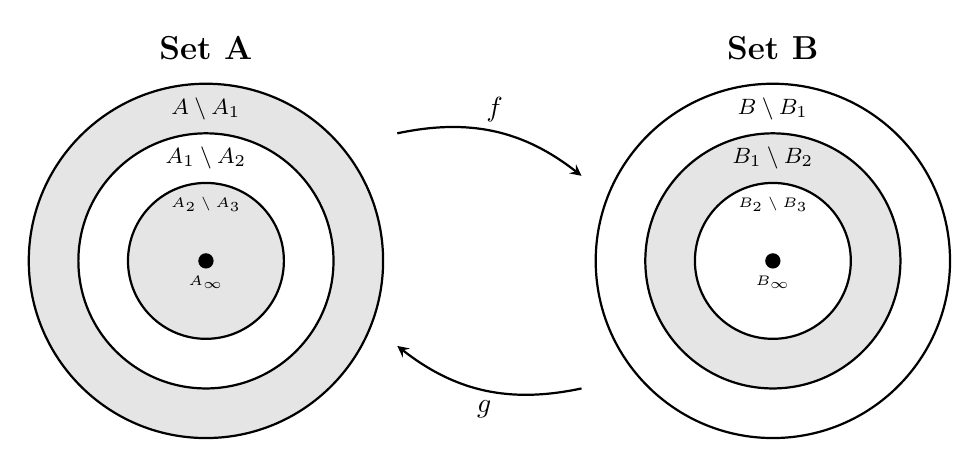
\begin{tikzpicture}[scale=0.9, >=stealth]
    % === SET A (left) ===
    % Pattern: GRAY - WHITE - GRAY
    \node at (-4, 3.0) {\large \textbf{Set A}};

    % 1. Outer layer (gray) - goes to B
    \draw[thick, fill=gray!20] (-4,0) circle (2.5cm);
    \node at (-4, 2.15) {\footnotesize $A \setminus A_1$};

    % 2. Middle layer (white) - comes from B
    \draw[thick, fill=white] (-4,0) circle (1.8cm);
    \node at (-4, 1.45) {\footnotesize $A_1 \setminus A_2$};

    % 3. Inner layer (gray) - goes to B
    \draw[thick, fill=gray!20] (-4,0) circle (1.1cm);
    \node at (-4, 0.8) {\tiny $A_2 \setminus A_3$};

    % Core
    \draw[fill=black] (-4,0) circle (0.1cm);
    \node at (-4, -0.3) {\tiny $A_\infty$};

    % === SET B (right) ===
    % INVERTED pattern: WHITE - GRAY - WHITE
    \node at (4, 3.0) {\large \textbf{Set B}};

    % 1. Outer layer (white) - goes to A
    \draw[thick, fill=white] (4,0) circle (2.5cm);
    \node at (4, 2.15) {\footnotesize $B \setminus B_1$};

    % 2. Middle layer (gray) - comes from A
    \draw[thick, fill=gray!20] (4,0) circle (1.8cm);
    \node at (4, 1.45) {\footnotesize $B_1 \setminus B_2$};

    % 3. Inner layer (white) - goes to A
    \draw[thick, fill=white] (4,0) circle (1.1cm);
    \node at (4, 0.8) {\tiny $B_2 \setminus B_3$};

    % Core
    \draw[fill=black] (4,0) circle (0.1cm);
    \node at (4, -0.3) {\tiny $B_\infty$};

    % Arrow f: leaves GRAY (A) -> enters GRAY (B)
    \draw[->, thick] (-1.3, 1.8) to[bend left=25] node[midway, above] {$f$} (1.3, 1.2);

    % Arrow g: leaves WHITE (B) -> enters WHITE (A)
    \draw[->, thick] (1.3, -1.8) to[bend left=25] node[midway, below] {$g$} (-1.3, -1.2);

\end{tikzpicture}
\end{figure}

\begin{proof}
Define recursively
\begin{align*}
    A_1 &= g(B) & B_1 &= f(A) \\
    A_2 &= g(B_1) & B_2 &= f(A_1) \\
    &\vdots & &\vdots \\
    A_{k+1} &= g(B_k) & B_{k+1} &= f(A_k) \\
    A_\infty &= \bigcap_{k=1}^{\infty} A_k \quad & \quad B_\infty &= \bigcap_{k=1}^{\infty} B_k.
\end{align*}

$A$ and $B$ are written as disjoint unions of the layers and the cores, and $h$ acts
differently on each part.

\[
\setlength{\arraycolsep}{6pt}
\begin{array}{rcccl}
    % --- ROW OF SET A ---
    A \; = &
    \underbrace{\left[ (A \setminus A_1) \cup (A_2 \setminus A_3) \cup \dots \right]}_{\text{Even
    layers of A}} &
    \cup &
    \underbrace{\left[ (A_1 \setminus A_2) \cup (A_3 \setminus A_4) \cup \dots \right]}_{\text{Odd
    layers of A}} &
    \cup \underbrace{A_\infty}_{\text{Core of A}} \\

    % --- ROW OF ARROWS ---
    &
    \Bigg\downarrow f \quad \Bigg\uparrow f^{-1} &
    &
    \Bigg\downarrow g^{-1} \quad \Bigg\uparrow g &

    \hspace{0.5cm} \Bigg\downarrow f \quad \Bigg\uparrow f^{-1} \\

    % --- ROW OF SET B ---
    B \; = &
    \underbrace{\left[ (B_1 \setminus B_2) \cup (B_3 \setminus B_4) \cup \dots \right]}_{\text{Odd
    layers of B}} &
    \cup &
    \underbrace{\left[ (B \setminus B_1) \cup (B_2 \setminus B_3) \cup \dots \right]}_{\text{Even
    layers of B}} &
    \cup \underbrace{B_\infty}_{\text{Core of B}} \\
\end{array}
\]

Define $h: A \to B$ by cases:
$$
h(x) = \begin{cases}
    f(x) & \text{if } x \in A_k \setminus A_{k+1} \text{ with } k \text{ even,} \\
    g^{-1}(x) & \text{if } x \in A_k \setminus A_{k+1} \text{ with } k \text{ odd,} \\
    f(x) & \text{if } x \in A_\infty.
\end{cases}
$$

Injectivity follows from the injectivity of $f$ and $g$. It remains to check surjectivity on each part.

\begin{enumerate}
    \item \textit{Even rings.} The restriction
    $f: (A_{2k} \setminus A_{2k+1}) \to (B_{2k+1} \setminus B_{2k+2})$ is onto. If
    $y \in B_{2k+1} \setminus B_{2k+2}$, since $B_{2k+1} = f(A_{2k})$ there is $x \in A_{2k}$ with
    $f(x) = y$. If $x \in A_{2k+1}$, then $y = f(x) \in f(A_{2k+1}) = B_{2k+2}$, a contradiction.
    Hence $x \in A_{2k} \setminus A_{2k+1}$.

    \item \textit{Odd rings.} Now the restriction
    $g^{-1}: (A_{2k-1} \setminus A_{2k}) \to (B_{2k-2} \setminus B_{2k-1})$. It is equivalent to showing that
    $$ g: (B_{2k-2} \setminus B_{2k-1}) \to (A_{2k-1} \setminus A_{2k}) $$
    is a bijection. Take $x \in A_{2k-1} \setminus A_{2k}$; since $A_{2k-1} = g(B_{2k-2})$, there is
    $y \in B_{2k-2}$ with $g(y) = x$. If $y \in B_{2k-1}$, then
    $x = g(y) \in g(B_{2k-1}) = A_{2k}$, a contradiction.

    \item \textit{The core.} For $f: A_\infty \to B_\infty$, given $z \in B_\infty$,
    $z \in B_{k+1} = f(A_k)$ for every $k$. There are then $x_k \in A_k$ with $f(x_k) = z$; by
    injectivity of $f$ it is \emph{the same} $x$ for every $k$. Hence
    $x \in \bigcap A_k = A_\infty$ and $z = f(x)$.
\end{enumerate}
$h$ is a bijection and therefore $A \sim B$.
\end{proof}

\subsection{Algebra of Countable Sets}

\begin{teorema}{Cartesian Product}{prod_cart}
The finite Cartesian product of countable sets is countable. In particular,
$\mathbb{N} \times \mathbb{N} \sim \mathbb{N}$.
\end{teorema}
\begin{proof}
By induction on the number $k$ of factors. The case $k=1$ is the hypothesis: a single
factor, already countable. For the inductive step, by associativity
$$ A_1 \times \cdots \times A_n \times A_{n+1} = (A_1 \times \cdots \times A_n) \times A_{n+1} = P_n
\times A_{n+1}, $$
and everything reduces to showing that the product of two countable sets is countable. That in turn follows
from $\mathbb{N} \times \mathbb{N} \sim \mathbb{N}$: the function $f(n,m) = 2^n 3^m$ is
injective by the Fundamental Theorem of Arithmetic.
\end{proof}

\begin{teorema}{Countable Union}{union_num}
$$ A = \bigcup_{n \in \mathbb{N}} A_n, \quad \text{with } A_n \text{ countable} \implies A
\text{ is countable.} $$
\end{teorema}
\begin{proof}
If the $A_n$ are not disjoint, an element may be counted several times, which prevents building
a direct injection. Replace $(A_n)$ by a disjoint family with the same union:
$$ A'_1 = A_1, \qquad A'_n = A_n \setminus \bigcup_{k=1}^{n-1} A_k \quad (n > 1). $$
Each $A'_n \subseteq A_n$ is countable, the $A'_n$ are pairwise disjoint, and
$\bigcup A'_n = \bigcup A_n$.

Hence there are injections $g_n: A'_n \to \mathbb{N}$. Define
$H: A \to \mathbb{N} \times \mathbb{N}$: given $x \in A$, there is a unique $n$ with $x \in A'_n$ (because
they are disjoint), and set $H(x) = (n, g_n(x))$. $H$ is injective. Since
$\mathbb{N} \times \mathbb{N} \sim \mathbb{N}$, $A$ is countable.
\end{proof}

\begin{teorema}{Rationals}{racionales}
$\mathbb{Q}$ is countable.
\end{teorema}
\begin{proof}
By means of the assignment $p/q \mapsto (p, q)$ (with $q \in \mathbb{N}$, $p \in \mathbb{Z}$ and $\gcd(p,q)=1$),
$\mathbb{Q}$ injects into $\mathbb{Z} \times \mathbb{N}$, which is countable.
\end{proof}

\subsection{Uncountable Sets}

\begin{teorema}{Uncountability of the Interval}{intervalo_no_num}
The interval $(0,1)$ is not countable.
\end{teorema}

\begin{proof}
By Cantor's diagonal argument. If it were countable, its elements could be listed:
\begin{align*}
y_1 &= 0.d_{11}d_{12}d_{13}\dots \\
y_2 &= 0.d_{21}d_{22}d_{23}\dots \\
\vdots & \\
y_k &= 0.d_{k1}d_{k2}d_{k3}\dots
\end{align*}
Construct $z = 0.z_1z_2z_3\dots$ with $z_k \ne d_{kk}$ (for example, $z_k = 2$ if $d_{kk}=1$ and
$z_k = 1$ otherwise). Then $z$ differs from each $y_k$ in the $k$-th digit, so that
$z \notin \{y_k\}$, contrary to the assumption that the list covered $(0,1)$.
\end{proof}

\begin{corolario}{Reals}{reales}
$\mathbb{R}$ is not countable.
\end{corolario}

\begin{proof}
First, $(0,1) \sim (a,b)$ via the linear map $t \mapsto a + t(b-a)$. Second,
$\mathbb{R} \sim (-\pi/2, \pi/2)$ via $\arctan$. Composition gives $\mathbb{R} \sim (0,1)$, which is not
countable.
\end{proof}

\subsection*{A remark on notation and the order of cardinals}

\begin{lema}[Injectivity and Surjectivity by Composition]\label{lema:iny_sob_comp}
If $f: A \to B$, $g: B \to A$ and $g \circ f = \mathrm{id}_A$, then $f$ is injective and $g$ is
surjective.
\end{lema}

\begin{proof}
\textit{$f$ injective.} If $f(x_1) = f(x_2)$, applying $g$ gives $x_1 = g(f(x_1)) = g(f(x_2)) = x_2$.

\textit{$g$ surjective.} Given $a \in A$, take $b = f(a)$; then $g(b) = a$.
\end{proof}

With this, the order of cardinals is defined:

\begin{definicion}{Inequality of Cardinals}{}
$\#A \le \#B$ if there is an injection $f: A \to B$.
\end{definicion}

There is an equivalent formulation with surjections in the other direction:

\begin{proposicion}{Equivalent Form of $\#A \le \#B$}{}
If $A \ne \emptyset$, $\#A \le \#B$ if and only if there is a surjection $g: B \to A$.
\end{proposicion}

\begin{proof}
Both implications are proved.

\textit{($\Rightarrow$).} Let $f: A \to B$ be injective. Define $g: B \to A$: for $b \in f(A)$,
let $g(b)$ be the unique $a$ with $f(a) = b$, and for $b \notin f(A)$ assign a fixed $a_0 \in A$
(here $A \ne \emptyset$ is used). Thus $g \circ f = \mathrm{id}_A$ and, by
Lemma~\ref{lema:iny_sob_comp}, $g$ is surjective.

\textit{($\Leftarrow$).} Let $g$ be surjective. By the axiom of choice, for each $a$ choose
$b_a \in g^{-1}(\{a\})$ and define $f(a) = b_a$. Then $g \circ f = \mathrm{id}_A$ and $f$ is
injective.
\end{proof}


\subsection{Cantor's Theorem (Power Set)}

\begin{teorema}{Cantor's Theorem}{potencia}
$|A| < |\mathcal{P}(A)|$ for every set $A$.
\end{teorema}

\begin{proof}
$|A| \le |\mathcal{P}(A)|$ because $a \mapsto \{a\}$ is injective. To see that there is no surjection
$h: A \to \mathcal{P}(A)$, argue by contradiction (diagonal argument): if $h$ were onto, with the
diagonal set
$$ B = \{ x \in A : x \notin h(x) \} \in \mathcal{P}(A) $$
there would be $b \in A$ with $h(b) = B$. But
\begin{itemize}
    \item $b \in B \implies b \notin h(b) = B$,
    \item $b \notin B \implies b \in h(b) = B$.
\end{itemize}
Both are absurd, so that no such $h$ exists.
\end{proof}

\newpage

\subsection{Solved exercises}

\subsection*{Exercise 1}

Let $A$ and $B$ be subsets of $X$.

\begin{proposicion}{Exercise 1.i}{ej1_i}
Prove that $A \subset B \iff B^c \subset A^c$.
\end{proposicion}

\begin{proof}
Both implications are proved.

\textit{($\Rightarrow$).} Suppose that $A \subset B$; it must be shown that $B^c \subset A^c$.
\begin{itemize}
    \item Let $x \in B^c$, that is, $x \notin B$.
    \item By hypothesis $A \subset B$, so that if $x$ were in $A$ it would be in $B$.
    \item Since $x \notin B$, by contraposition $x \notin A$.
    \item If $x \notin A$, then $x \in A^c$.
\end{itemize}

\textit{($\Leftarrow$).} Suppose that $B^c \subset A^c$; it must be shown that $A \subset B$.
\begin{itemize}
    \item Let $x \in A$, that is, $x \notin A^c$.
    \item By hypothesis ($B^c \subset A^c$), if $x$ belonged to $B^c$ it would belong to $A^c$.
    \item Since $x \notin A^c$, it cannot be that $x \in B^c$.
    \item Therefore $x \notin B^c$, which implies $x \in B$.
\end{itemize}
\end{proof}

\begin{proposicion}{Exercise 1.ii}{ej1_ii}
Prove that $B - \bigcup_{i} A_i = \bigcap_{i} (B - A_i)$.
\end{proposicion}

\begin{proof}
Double inclusion is proved.

\textit{($\subseteq$).} Let $x \in B - \bigcup_{i} A_i$.
\begin{itemize}
    \item By definition of difference, $x \in B$ \emph{and} $x \notin \bigcup_{i} A_i$.
    \item That $x$ is not in the union means that it belongs to none of the $A_i$; that is,
    $\forall i, x \notin A_i$.
    \item Since $x \in B$ and moreover $\forall i, x \notin A_i$,
    $\forall i, (x \in B \land x \notin A_i)$.
    \item This is equivalent to $\forall i, x \in (B - A_i)$.
    \item By definition of generalized intersection, $x \in \bigcap_{i} (B - A_i)$.
\end{itemize}

\textit{($\supseteq$).} Let $x \in \bigcap_{i} (B - A_i)$.
\begin{itemize}
    \item By definition of intersection, $\forall i, x \in (B - A_i)$.
    \item That is, for every $i$: $x \in B$ \emph{and} $x \notin A_i$.
    \item Two things follow from this:
    \begin{enumerate}
        \item $x \in B$ (common to all).
        \item $\forall i, x \notin A_i$.
    \end{enumerate}
    \item The second condition implies that there is no index with $x \in A_i$; therefore
    $x \notin \bigcup_{i} A_i$.
    \item Putting together $x \in B$ and $x \notin \bigcup_{i} A_i$, one obtains $x \in B - \bigcup_{i} A_i$.
\end{itemize}
\end{proof}

\begin{proposicion}{Exercise 1.iii}{ej1_iii}
Prove that $B - \bigcap_{i} A_i = \bigcup_{i} (B - A_i)$.
\end{proposicion}

\begin{proof}
Double inclusion is proved.

\textit{($\subseteq$).} Let $x \in B - \bigcap_{i} A_i$.
\begin{itemize}
    \item Then $x \in B$ \emph{and} $x \notin \bigcap_{i} A_i$.
    \item Denying that $x$ is in the intersection means that it fails for at least one: there is some
    index $k$ with $x \notin A_k$.
    \item Since $x \in B$ and for that $k$ one has $x \notin A_k$, then $x \in (B - A_k)$.
    \item Since $x$ belongs to one of the sets of the family, it belongs to the union.
\end{itemize}

\textit{($\supseteq$).} Let $x \in \bigcup_{i} (B - A_i)$.
\begin{itemize}
    \item By definition of union, there is some index $k$ with $x \in (B - A_k)$.
    \item That is, $x \in B$ and $x \notin A_k$.
    \item Since $x \notin A_k$, $x$ cannot be in the intersection of all the $A_i$ (since $x \notin A_k$). Therefore $x \notin \bigcap_{i} A_i$.
    \item Having $x \in B$ and $x \notin \bigcap_{i} A_i$, it follows that $x \in B - \bigcap_{i} A_i$.
\end{itemize}
\end{proof}

\begin{proposicion}{Exercise 1.iv}{ej1_iv}
Prove that $\bigcup_{i} (A_i \cap B) = (\bigcup_{i} A_i) \cap B$.
\end{proposicion}

\begin{proof}
Double inclusion is proved.

\textit{($\subseteq$).} Let $x \in \bigcup_{i} (A_i \cap B)$.
\begin{itemize}
    \item There is some index $k$ with $x \in (A_k \cap B)$.
    \item That is, $x \in A_k$ and $x \in B$.
    \item Since $x \in A_k$, then $x \in \bigcup_{i} A_i$ (being in one suffices).
    \item Since $x \in \bigcup_{i} A_i$ and moreover $x \in B$, then $x \in (\bigcup_{i} A_i) \cap B$.
\end{itemize}

\textit{($\supseteq$).} Let $x \in (\bigcup_{i} A_i) \cap B$.
\begin{itemize}
    \item Then $x \in \bigcup_{i} A_i$ and $x \in B$.
    \item Being in the union, there is an index $k$ with $x \in A_k$.
    \item Since $x \in A_k$ and $x \in B$, then $x \in (A_k \cap B)$.
    \item Belonging to one of the terms $(A_k \cap B)$, it belongs to the union.
\end{itemize}
\end{proof}

\subsection*{Exercise 2}

Given a sequence $(A_{n})_{n\in\mathbb{N}}$ of sets, and $A=\bigcup_{n}A_{n}$, find a
sequence $(B_{n})_{n\in\mathbb{N}}$ of disjoint sets such that $A=\bigcup_{n}B_{n}$.

\begin{proof}
Define the sequence $(B_n)$ recursively:
$$ B_1 = A_1 $$
$$ B_n = A_n \setminus \left( \bigcup_{k=1}^{n-1} A_k \right) \quad \text{for } n > 1 $$

Two things must be proved: that they are disjoint and that their union is $A$.

\textit{Disjoint.} Let $n, m \in \mathbb{N}$ with $n \neq m$; without loss of generality, $m < n$.
By definition,
$$ B_n = A_n \setminus (A_1 \cup \dots \cup A_m \cup \dots \cup A_{n-1}), $$
so that $B_n$ has no element of $A_m$, that is, $B_n \cap A_m = \emptyset$. Since
$B_m \subseteq A_m$ by construction, one has $B_n \cap B_m = \emptyset$.

\textit{Equality of the unions.} Double inclusion is proved.

$(\subseteq)$ Since $B_n \subseteq A_n$ for every $n$,
$$ \bigcup_{n=1}^{\infty} B_n \subseteq \bigcup_{n=1}^{\infty} A_n = A. $$

$(\supseteq)$ Let $x \in A = \bigcup_{n=1}^{\infty} A_n$; then $x$ belongs to at least one of the
$A_n$. Let $k$ be the least index with $x \in A_k$. This implies $x \in A_k$ and $x \notin A_j$ for every
$j < k$ (otherwise, $k$ would not be the least). Hence $x$ does not belong to the union of the previous ones:
$$ x \notin \bigcup_{j=1}^{k-1} A_j, $$
and by definition of $B_k$ one has $x \in A_k \setminus \bigcup_{j=1}^{k-1} A_j$, that is,
$x \in B_k$. Therefore $x \in \bigcup_{n=1}^{\infty} B_n$.

Finally, $A=\bigcup_{n}B_{n}$.
\end{proof}

\subsection*{Exercise 3}

Given a function $f:X\longrightarrow Y$ and subsets $A, B$ of $X$ and $C, D$ of $Y$.

\begin{proposicion}{3.i}{ej3_i}
$f(A\cup B)=f(A)\cup f(B)$
\end{proposicion}

\begin{proof}
Double inclusion is proved.

\textit{($\subseteq$).} Let $y \in f(A \cup B)$. By definition of direct image, there is
$x \in A \cup B$ with $f(x) = y$. Since $x \in A$ or $x \in B$:
\begin{itemize}
    \item if $x \in A$, then $f(x) \in f(A)$, hence $y \in f(A)$;
    \item if $x \in B$, then $f(x) \in f(B)$, hence $y \in f(B)$.
\end{itemize}
In either case, $y \in f(A) \cup f(B)$.

\textit{($\supseteq$).} Let $y \in f(A) \cup f(B)$, that is, $y \in f(A)$ or $y \in f(B)$.
\begin{itemize}
    \item If $y \in f(A)$, there is $x \in A$ with $f(x) = y$. Since $A \subset A \cup B$, then
    $x \in A \cup B$, so that $y \in f(A \cup B)$.
    \item Analogously, if $y \in f(B)$, there is $x \in B$ with $f(x) = y$, and $y \in f(A \cup B)$.
\end{itemize}
\end{proof}

\begin{proposicion}{3.ii}{ej3_ii}
$f(A\cap B)\subset f(A)\cap f(B)$. Does equality hold?
\end{proposicion}

\begin{proof}
Let $y \in f(A \cap B)$. There is $x \in A \cap B$ with $f(x) = y$. Since $x \in A$ and $x \in B$, one has
$f(x) \in f(A)$ and $f(x) \in f(B)$, hence $y \in f(A) \cap f(B)$.
\end{proof}

Equality does not hold in general. As a counterexample, let $f: \mathbb{R} \to \mathbb{R}$, $f(x) = x^2$,
and let $A = [-1, 0]$, $B = [0, 1]$. Then $A \cap B = \{0\}$, so that $f(A \cap B) = \{0\}$;
on the other hand $f(A) = [0, 1] = f(B)$, so that $f(A) \cap f(B) = [0, 1] \neq \{0\}$.

\begin{proposicion}{3.iii}{ej3_iii}
$f^{-1}(C\cup D)=f^{-1}(C)\cup f^{-1}(D)$
\end{proposicion}

\begin{proof}
Let $x$ be an arbitrary element:
\begin{align*}
x \in f^{-1}(C \cup D) &\iff f(x) \in C \cup D \\
&\iff f(x) \in C \lor f(x) \in D \\
&\iff x \in f^{-1}(C) \lor x \in f^{-1}(D) \\
&\iff x \in f^{-1}(C) \cup f^{-1}(D). \qedhere
\end{align*}
\end{proof}

\begin{proposicion}{3.iv}{ej3_iv}
$f^{-1}(C\cap D)=f^{-1}(C)\cap f^{-1}(D)$
\end{proposicion}

\begin{proof}
Let $x$ be an arbitrary element:
\begin{align*}
x \in f^{-1}(C \cap D) &\iff f(x) \in C \cap D \\
&\iff f(x) \in C \land f(x) \in D \\
&\iff x \in f^{-1}(C) \land x \in f^{-1}(D) \\
&\iff x \in f^{-1}(C) \cap f^{-1}(D). \qedhere
\end{align*}
\end{proof}

\begin{proposicion}{3.v}{ej3_v}
$A\subset f^{-1}(f(A))$. Does equality hold?
\end{proposicion}

\begin{proof}
Let $x \in A$. Applying $f$, $f(x) \in f(A)$. By definition of preimage, $f^{-1}(f(A))$ contains
all the elements whose image lies in $f(A)$; since $f(x) \in f(A)$, then $x \in f^{-1}(f(A))$.
\end{proof}

Equality does not hold in general (only if $f$ is injective). As a counterexample, let $f(x) = x^2$ and
$A = \{1\}$: then $f(A) = \{1\}$ and $f^{-1}(f(A)) = f^{-1}(\{1\}) = \{-1, 1\}$, with
$\{1\} \subsetneq \{-1, 1\}$.

\begin{proposicion}{3.vi}{ej3_vi}
$f(f^{-1}(C))\subset C$. Does equality hold?
\end{proposicion}

\begin{proof}
Let $y \in f(f^{-1}(C))$. By definition of direct image, there is $x \in f^{-1}(C)$ with $f(x) = y$;
and by definition of preimage, $x \in f^{-1}(C)$ implies $f(x) \in C$. Since $f(x) = y$, it follows that
$y \in C$.
\end{proof}

Equality does not hold in general (only if $f$ is surjective or if $C \subset \operatorname{Im}(f)$).
As a counterexample, let $f(x) = e^x$ from $\mathbb{R}$ to $\mathbb{R}$ and $C = \mathbb{R}$: then
$f^{-1}(C) = \mathbb{R}$ and $f(f^{-1}(C)) = f(\mathbb{R}) = (0, \infty)$, with
$(0, \infty) \subsetneq \mathbb{R}$.

\begin{proposicion}{3.vii}{ej3_vii}
$f^{-1}(D^c) = (f^{-1}(D))^c$
\end{proposicion}

\begin{proof}
Let $x$ be an arbitrary element:
\begin{align*}
x \in f^{-1}(D^c) &\iff f(x) \in D^c \\
&\iff f(x) \notin D \\
&\iff \neg (f(x) \in D) \\
&\iff \neg (x \in f^{-1}(D)) \\
&\iff x \notin f^{-1}(D) \\
&\iff x \in (f^{-1}(D))^c. \qedhere
\end{align*}
\end{proof}

\subsection*{Exercise 4}

\begin{proposicion}{Relation $\to$ Partition}{ej4_rel_part}
Let $X$ be a set and $\sim$ an equivalence relation on $X$.
The set of equivalence classes (quotient set) $X/\sim = \{ [x] : x \in X \}$ forms a
partition of $X$.
\end{proposicion}

\begin{proof}
A family of sets is a partition if it satisfies three conditions.

\textit{The classes are nonempty.} Let $[x]$ be an arbitrary class. By reflexivity, $x \sim x$, and
by definition of class ($[x] = \{y \in X : y \sim x\}$) this gives $x \in [x]$. Hence
$[x] \neq \emptyset$.

\textit{The union covers $X$.} The union of subsets of $X$ is contained in $X$. For the other
inclusion, let $x \in X$; since $x \in [x]$, the element $x$ belongs to the union of all the classes.
Therefore
$$ X = \bigcup_{x \in X} [x]. $$

\textit{They are pairwise disjoint.} Let $[x]$ and $[y]$ be two classes; it must be shown that they are disjoint or
identical. Suppose that they are not disjoint, that is, there is $z \in [x] \cap [y]$.
\begin{itemize}
    \item $z \in [x] \implies z \sim x \implies x \sim z$.
    \item $z \in [y] \implies z \sim y$.
    \item By transitivity, $x \sim y$.
\end{itemize}
Now it is shown that $[x] = [y]$. Let $w \in [x]$, that is $w \sim x$; since $w \sim x$ and $x \sim y$, by
transitivity $w \sim y$, hence $w \in [y]$. This proves $[x] \subseteq [y]$, and by symmetry the
opposite inclusion holds. Thus, two classes that share an element are equal; if they are distinct, their
intersection is empty.
\end{proof}

\begin{proposicion}{Partition $\to$ Relation}{ej4_part_rel}
Let $P = \{A_i\}_{i \in I}$ be a partition of a set $X$.
The relation defined by $x \sim y \iff \exists k \in I$ such that $x \in A_k \land y \in A_k$ is an
equivalence relation.
\end{proposicion}

\begin{proof}
The three properties are verified.

\textit{Reflexivity.} Let $x \in X$. Since $P$ is a partition, the union of the $A_i$ covers $X$, so
that there is an index $k$ with $x \in A_k$. Then $x$ and $x$ are in the same $A_k$, hence
$x \sim x$.

\textit{Symmetry.} Suppose $x \sim y$, that is, there is $k$ with $x, y \in A_k$. Then also
$y, x \in A_k$, hence $y \sim x$.

\textit{Transitivity.} Suppose $x \sim y$ and $y \sim z$.
\begin{itemize}
    \item $x \sim y \implies \exists k$ with $x, y \in A_k$.
    \item $y \sim z \implies \exists j$ with $y, z \in A_j$.
\end{itemize}
The element $y$ belongs both to $A_k$ and to $A_j$. Since the elements of $P$ are pairwise
disjoint, the only way for $A_k \cap A_j \neq \emptyset$ is $A_k = A_j$. Hence $x$ and $z$ are in the
same set, and $x \sim z$.
\end{proof}

\subsection*{Exercise 5}

This exercise has already been solved.

\subsection*{Exercise 6}

The exercise proposes using the principle of complete induction.
Given a property $P(n)$, define the truth set
$S = \{n \in \mathbb{N} : P(n) \text{ is true}\}$.
If it is proved that $1 \in S$ and that the property holding for all the previous ones implies that
it holds for the next one, then $S = \mathbb{N}$ (the formula holds for all of them).

\begin{proposicion}{6.i}{ej6_i}
$$ \sum_{k=1}^{n}k=\frac{n(n+1)}{2} $$
\end{proposicion}

\begin{proof}
By induction on $n$. Let $S = \{ n \in \mathbb{N} : \sum_{k=1}^{n}k=\frac{n(n+1)}{2} \}$.

\textit{Base case ($n=1$).} The left-hand side is $\sum_{k=1}^{1} k = 1$ and the right-hand side is
$\frac{1(1+1)}{2} = \frac{2}{2} = 1$. Since they coincide, $1 \in S$.

\textit{Inductive step.} Suppose that $n \in S$; it must be proved that
$\sum_{k=1}^{n+1}k = \frac{(n+1)(n+2)}{2}$. Starting from the sum up to $n+1$,
$$ \sum_{k=1}^{n+1}k = \left( \sum_{k=1}^{n}k \right) + (n+1). $$
Using the inductive hypothesis on the sum up to $n$,
$$ = \frac{n(n+1)}{2} + (n+1). $$
Factoring out $(n+1)$ and simplifying,
$$ = (n+1) \left( \frac{n}{2} + 1 \right) = (n+1) \left( \frac{n+2}{2} \right) = \frac{(n+1)(n+2)}{2}. $$
Hence $n+1 \in S$, and by induction $S = \mathbb{N}$.
\end{proof}

\begin{proposicion}{6.ii}{ej6_ii}
$$ \sum_{k=0}^{n}r^{k}=\frac{r^{n+1}-1}{r-1} \quad (r \neq 1) $$
\end{proposicion}

\begin{proof}
By induction on $n$. Let $S = \{ n \in \mathbb{N} : \sum_{k=0}^{n}r^{k}=\frac{r^{n+1}-1}{r-1} \}$.

\textit{Base case ($n=1$).} The left-hand side is $\sum_{k=0}^{1} r^k = r^0 + r^1 = 1 + r$ and the
right-hand side $\frac{r^{1+1}-1}{r-1} = \frac{r^2-1}{r-1} = \frac{(r-1)(r+1)}{r-1} = r+1$. Since they coincide,
$1 \in S$.

\textit{Inductive step.} Suppose that $n \in S$; it must be proved that the sum up to $n+1$ equals
$\frac{r^{n+2}-1}{r-1}$. Starting from the sum,
$$ \sum_{k=0}^{n+1} r^k = \left( \sum_{k=0}^{n} r^k \right) + r^{n+1}, $$
using the inductive hypothesis,
$$ = \frac{r^{n+1}-1}{r-1} + r^{n+1}, $$
and taking a common denominator, distributing and cancelling $r^{n+1}$ with $-r^{n+1}$,
$$ = \frac{r^{n+1}-1 + r^{n+1}(r-1)}{r-1} = \frac{r^{n+1} - 1 + r^{n+2} - r^{n+1}}{r-1}
= \frac{r^{n+2} - 1}{r-1}. $$
This is the formula at $n+1$, hence $n+1 \in S$ and by induction $S = \mathbb{N}$.
\end{proof}

\subsection*{Exercise 7}

Prove the Well-Ordering Principle: every nonempty subset of $\mathbb{N}$ has a minimum.

\begin{proof}
Argue by contradiction. Let $A \subseteq \mathbb{N}$ be nonempty and suppose that $A$ has no minimum.
Define the set of naturals strictly smaller than every element of $A$:
$$ S = \{ n \in \mathbb{N} : \forall a \in A,\ n < a \}. $$
It is proved by induction that $S = \mathbb{N}$.

\textit{Base case.} Since $1$ is the least natural ($1 \le x$ for every $x \in \mathbb{N}$), if
$1 \in A$ then $1$ would be the minimum of $A$. Since $A$ has no minimum, $1 \notin A$; hence
$\{1\} \cap A = \emptyset$, which gives $1 \in S$.

\textit{Inductive step.} Suppose $n \in S$, that is, $\{1, 2, \dots, n\} \cap A = \emptyset$. If
$n+1 \in A$, since $1, \dots, n$ are not in $A$, then $n+1$ would be the minimum of $A$, which does not
exist. Therefore $n+1 \notin A$, so that $\{1, 2, \dots, n, n+1\} \cap A = \emptyset$ and
$n+1 \in S$.

By induction, $S = \mathbb{N}$, that is, $n \notin A$ for every natural $n$, and consequently
$A = \emptyset$. This contradicts $A$ being nonempty. The contradiction comes from supposing that $A$
has no minimum; hence $A$ has a minimum.
\end{proof}

\subsection*{Exercise 8}

Find the cardinality of the following sets.

\begin{itemize}
    \item Set: $\mathbb{Z}_{\ge 3} = \{ n \in \mathbb{Z} : n \ge 3 \}$.
    Cardinality: $\aleph_0$.
    \\ It is an infinite subset of a countable set ($\mathbb{Z}$), therefore it is
    countable. The explicit bijection $f: \mathbb{N} \to \mathbb{Z}_{\ge 3}$ is given
    by $f(n) = n + 2$.

    \item Set: $5\mathbb{Z} = \{ 5k : k \in \mathbb{Z} \}$.
    Cardinality: $\aleph_0$.
    \\ Define the function $f: \mathbb{Z} \to 5\mathbb{Z}$ as $f(k) = 5k$, which is bijective
    (injective because $5k_1=5k_2 \implies k_1=k_2$ and surjective by definition). Since
    $\mathbb{Z} \sim \mathbb{N}$, then $5\mathbb{Z} \sim \mathbb{N}$.

    \item Set: $\mathbb{Z} \times \mathbb{N}$.
    Cardinality: $\aleph_0$.
    \\ Both $\mathbb{Z}$ and $\mathbb{N}$ are countable. By Theorem \ref{teo:prod_cart}, the
    finite Cartesian product of countable sets is countable.

    \item Set: $\mathbb{R} - \mathbb{Q}$.
    Cardinality: $c$.
    \\ One has $\mathbb{R} = (\mathbb{R} - \mathbb{Q}) \cup \mathbb{Q}$. By contradiction: if the irrationals were
    countable, since $\mathbb{Q}$ is countable, $\mathbb{R}$ would be a union of two countable sets, and
    hence countable; this contradicts the uncountability of the reals. Hence
    $\mathbb{R} - \mathbb{Q}$ is uncountable.

    \item Set: $(-1, 1) \cap \mathbb{Q}$.
    Cardinality: $\aleph_0$.
    \\ It is a subset of $\mathbb{Q}$, and every subset of a countable set is at most
    countable.
\end{itemize}

\subsection*{Exercise 9}

Prove that the set of prime numbers is countable.

\begin{proof}
Let $P$ be the set of prime numbers. Since $P \subset \mathbb{N}$, it suffices to see that it is infinite.
Argue by contradiction: suppose that there are finitely many primes $p_1, p_2, \dots, p_n$, and
consider
$$ Q = (p_1 \cdot p_2 \cdot \dots \cdot p_n) + 1. $$
The number $Q$ has some prime divisor $q$.
\begin{itemize}
    \item If $q$ were one of the primes in the list, $q$ would divide the product $p_1 \dots p_n$.
    \item Since $q$ divides $Q$ and the product, it divides the difference $Q - (p_1 \dots p_n) = 1$.
    \item But a prime cannot divide $1$.
\end{itemize}
This is a contradiction, so that there are infinitely many primes. Being an infinite subset of
$\mathbb{N}$, $P$ is countable.
\end{proof}

\subsection*{Exercise 10}

Prove that $P(A) \sim \{0,1\}^{A}$. Become convinced that $\mathbb{R} \sim P(\mathbb{N})$ and that there are
more real numbers than naturals.

\begin{proposicion}{Equipotence of Power Set and Characteristic Functions}{ej10}
The power set of $A$, denoted $P(A)$, is equipotent with the set of functions from $A$ to
$\{0,1\}$, denoted $\{0,1\}^A$.
\end{proposicion}

\begin{proof}
Define the function $\Phi: P(A) \to \{0,1\}^A$ that assigns to each subset $B \subseteq A$ its
characteristic function $\chi_B$, where
$$ \chi_B(x) = \begin{cases} 1 & \text{if } x \in B \\ 0 & \text{if } x \notin B. \end{cases} $$
It is shown that $\Phi$ is bijective.

\textit{Injectivity.} Let $B, C \subseteq A$ with $\Phi(B) = \Phi(C)$, that is,
$\chi_B(x) = \chi_C(x)$ for every $x \in A$. Then
$$ x \in B \iff \chi_B(x) = 1 \iff \chi_C(x) = 1 \iff x \in C, $$
hence $B = C$.

\textit{Surjectivity.} Let $f: A \to \{0,1\}$ be an arbitrary function. A set $B$ whose characteristic
function is $f$ is sought; define the set of elements that $f$ sends to $1$:
$$ B = \{ x \in A : f(x) = 1 \}. $$
Then $B \subseteq A$, so that $B \in P(A)$. By construction,
$\chi_B(x) = 1 \iff x \in B \iff f(x) = 1$ and $\chi_B(x) = 0 \iff x \notin B \iff f(x) = 0$, so that
$\Phi(B) = f$.

Hence $\Phi$ is a bijection and $P(A) \sim \{0,1\}^A$.
\end{proof}

To become convinced that $\mathbb{R} \sim P(\mathbb{N})$:
\begin{itemize}
    \item It was already proved that $P(\mathbb{N}) \sim \{0,1\}^{\mathbb{N}}$.
    \item The elements of $\{0,1\}^{\mathbb{N}}$ are infinite sequences of zeros and ones (for
    example $0, 1, 1, 0, \dots$).
    \item The real numbers in $(0,1)$ are represented by their binary expansion
    $$ x = 0.d_1 d_2 d_3 \dots \quad \text{with } d_i \in \{0,1\}. $$
    \item There is an almost bijective correspondence between these sequences and the reals (except for the cases
    of double representation, such as $0.100\dots = 0.011\dots$).
    \item Therefore the cardinality of $\mathbb{R}$ coincides with that of the binary sequences, which is
    that of the power set of $\mathbb{N}$.
    \item Since by Cantor's Theorem~\ref{teo:potencia}, $|P(\mathbb{N})| > |\mathbb{N}|$, there are
    strictly more reals than naturals.
\end{itemize}

\subsection*{Exercise 11}

Given $B \subset \mathbb{N}$, prove that if $B$ is equipotent with a proper subset of itself,
then $B$ is countable.

\begin{proof}
Let $B \subset \mathbb{N}$ be such that there exist $B' \subsetneq B$ and a bijection $f: B \to B'$. Since
$B \subseteq \mathbb{N}$, $B$ can only be finite or countable.

Suppose, by contradiction, that $B$ were finite. Two finite sets in bijection have the same cardinality, so that
$|B| = |B'|$; but since $B' \subsetneq B$ is a proper subset, $|B'| < |B|$. This gives the contradiction
$|B| < |B|$, so that $B$ cannot be finite.

Being an infinite subset of the naturals, $B$ is countable.
\end{proof}

\subsection*{Exercise 12}

Given a countable set $I$, prove that there is an uncountable family
$(I_{\alpha})_{\alpha \in A}$ of infinite subsets of $I$ such that for each
$\alpha \neq \beta$, the intersection $I_{\alpha} \cap I_{\beta}$ is finite.

\begin{proof}
Since $I$ is countable, it is identified with $\mathbb{Q}$. Take as index set the
reals ($A = \mathbb{R}$), which is uncountable.

For each $\alpha \in \mathbb{R}$ choose a sequence of distinct rationals
$(x_n)_{n \in \mathbb{N}}$ converging to $\alpha$, and define
$$ I_{\alpha} = \{ x_n : n \in \mathbb{N} \}. $$
Since the terms are distinct, each $I_{\alpha}$ is infinite.

Let $\alpha, \beta \in \mathbb{R}$ with $\alpha \neq \beta$. By contradiction, suppose that
$I_{\alpha} \cap I_{\beta}$ is infinite.
\begin{itemize}
    \item Let $S = I_{\alpha} \cap I_{\beta}$. Being infinite, its elements are ordered into a
    subsequence $(y_k)$.
    \item Since $S \subset I_{\alpha}$, the $y_k$ form a subsequence of the one converging to
    $\alpha$, hence $y_k \to \alpha$.
    \item Since $S \subset I_{\beta}$, the $y_k$ form a subsequence of the one converging to $\beta$,
    hence $y_k \to \beta$.
    \item By uniqueness of the limit (\ref{prop:unicidad}), $\alpha = \beta$.
\end{itemize}
This contradicts $\alpha \neq \beta$. Therefore $I_{\alpha} \cap I_{\beta}$ is finite.
\end{proof}

\newpage

\section{The real line}

\subsection{Bounds, Supremum and Maximum}

\begin{definicion}{Upper Bound, Supremum and Maximum}{cotas_sup}
Let $A \subseteq \mathbb{R}$.
\begin{itemize}
    \item \textbf{Upper bound:} $c \in \mathbb{R}$ with $a \le c$ for every $a \in A$. If one exists,
    $A$ is bounded above.
    \item \textbf{Supremum $s = \sup(A)$:} the least upper bound. It requires that $s$ be an upper bound and
    that every other upper bound $c$ satisfy $s \le c$.
    \item \textbf{Maximum $m = \max(A)$:} a supremum that belongs to the set.
\end{itemize}
\end{definicion}

Dually, for lower bounds:

\begin{definicion}{Lower Bound, Infimum and Minimum}{cotas_inf}
\textbf{Lower bound:} $c \le a$ for every $a \in A$. \textbf{Infimum:} the greatest lower bound,
$\inf(A)$. \textbf{Minimum:} an infimum that belongs to the set.
\end{definicion}

\obs One must distinguish between having bounds and having a maximum or minimum.
\begin{itemize}
    \item There may be no bounds (for example $\mathbb{N}$ is not bounded above), nor supremum, nor
    maximum.
    \item If there is an upper bound, there are infinitely many (any larger number is one as well). But if
    the supremum exists, it is unique.
    \item Having a maximum is stronger than having a supremum: $\max(A)$, when it exists, coincides with
    $\sup(A)$. But there may be a supremum without a maximum: $\sup [0,1) = 1$ and it is not a maximum.
\end{itemize}

\subsection{The Completeness Axiom}

\begin{teorema}{Completeness Axiom}{axioma_completitud}
Every nonempty $A \subset \mathbb{R}$ that is bounded above has a supremum in $\mathbb{R}$.
\end{teorema}

\obs In $\mathbb{Q}$ this fails. The set $\{x \in \mathbb{Q} : x^2 < 2\}$ is bounded by $2$
but its ``edge'' $\sqrt{2}$ is not rational.

\begin{proposicion}{Characterization of the Supremum}{carac_supremo}
Let $s$ be an upper bound of $A$. $s = \sup(A)$ if and only if for every $\epsilon > 0$ there is $a \in A$
with $s - \epsilon < a$.
\end{proposicion}

\begin{proof}
Both implications are proved.

\textit{($\Rightarrow$)} By contradiction: if it did not hold, there would be $\epsilon > 0$ such that
$a \le s - \epsilon$ for every $a \in A$, and then $s - \epsilon$ would be an upper bound
strictly smaller than $s$, a contradiction.

\textit{($\Leftarrow$)} Let $c$ be any upper bound; by contradiction, if $c < s$, taking
$\epsilon = s - c > 0$ the
hypothesis gives $a_0 \in A$ with $a_0 > s - \epsilon = c$, which contradicts $c$ being an upper
bound. Thus $s \le c$ for every upper bound.
\end{proof}

\begin{proposicion}{Monotonicity of the Supremum and Infimum}{monotonia_sup_inf}
If $A \subseteq B$ with $B$ bounded, then $\inf(B) \le \inf(A) \le \sup(A) \le \sup(B)$.
\end{proposicion}

\begin{proof}
If $a \in A$, then $a \in B$ and $a \le \sup(B)$, so that $\sup(B)$ is an upper bound of $A$ and
$\sup(A) \le \sup(B)$. The infima are analogous.
\end{proof}

\begin{proposicion}{Archimedean Property}{arquimediana}
For every $x \in \mathbb{R}$ there is $n \in \mathbb{N}$ with $n > x$. Equivalently, for every
$\epsilon > 0$ there is $n \in \mathbb{N}$ with $1/n < \epsilon$.
\end{proposicion}

\begin{proof}
Argue by contradiction: if $\mathbb{N}$ were bounded above, by the Completeness Axiom
\ref{teo:axioma_completitud} it would have a supremum $s$.
Then $s - 1$ is not an upper bound and there is $n \in \mathbb{N}$ with $n > s - 1$, which gives
$n + 1 > s$, contradicting $s$ being an upper bound. The equivalent form is obtained by taking
$x = 1/\epsilon$.
\end{proof}

\begin{proposicion}{Density of $\mathbb{Q}$ in $\mathbb{R}$}{densidad_Q}
Between two reals $x < y$ there is always a rational.
\end{proposicion}

\begin{proof}
By the Archimedean Property \ref{prop:arquimediana}, there is $n$ with $1/n < y - x$, that is
$ny - nx > 1$. Between two reals separated by
more than 1 there is always an integer $m$ (take $m$ the least integer greater than $nx$). Then
$nx < m < ny$, and dividing, $x < m/n < y$.
\end{proof}

\subsection{Sequences and Subsequences}

\begin{definicion}{Sequence}{sucesion}
A \textbf{sequence} of reals is a function $x: \mathbb{N} \to \mathbb{R}$, denoted
$(x_n)_{n \in \mathbb{N}}$.
\end{definicion}

\begin{definicion}{Subsequence}{subsucesion}
A \textbf{subsequence} of $(x_n)$ is $(x_{n_k})_{k \in \mathbb{N}}$, where $k \mapsto n_k$ is
strictly increasing.
\end{definicion}

\begin{ejemplo}{The Subsequence $1/2^k$}{ej_subsucesion}
From the harmonic sequence $x_n = 1/n$, taking $n_k = 2^k$ yields $x_{n_k} = 1/2^k$: an accelerated version
of the original.
\end{ejemplo}

\subsection{Limit of a Sequence}

\begin{definicion}{Limit}{limite_suc}
$(x_n)$ \textbf{converges} to $a$ (written $x_n \to a$ or $\lim x_n = a$) if
$$ \forall \epsilon > 0, \ \exists n_\epsilon \in \mathbb{N} : \ n \ge n_\epsilon \implies |x_n - a|
< \epsilon. $$
\end{definicion}

$|x_n - a| < \epsilon$ is equivalent to $x_n \in (a - \epsilon, a + \epsilon)$. However small the
neighborhood around $a$, the sequence eventually enters it and stays: finitely many
terms may remain outside (the first $n_\epsilon - 1$), but all the others are inside.

\subsection{Boundedness and Uniqueness}

\begin{proposicion}{Convergence Implies Boundedness}{conv_acotada}
Every convergent sequence is bounded.
\end{proposicion}

\begin{proof}
Let $x_n \to a$. For $\epsilon = 1$ there is $n_0$ with $|x_n - a| < 1$ for every $n \ge n_0$. The
previous ones $\{x_1, \dots, x_{n_0-1}\}$ are finitely many: taking
$M = \max(\{a+1\} \cup \{x_1, \dots, x_{n_0-1}\})$ and $m$ analogously, $m \le x_n \le M$ for every $n$.
\end{proof}

\begin{proposicion}{Uniqueness of the Limit}{unicidad}
If $(x_n)$ converges, the limit is unique.
\end{proposicion}

\begin{proof}
Argue by contradiction: suppose $x_n \to a$ and $x_n \to b$ with $a \ne b$, and take
$\epsilon = |a-b|/2 > 0$. For large $n$,
$|x_n - a| < \epsilon$ and $|x_n - b| < \epsilon$, and by the triangle inequality
$$ |a - b| \le |a - x_n| + |x_n - b| < 2\epsilon = |a-b|, $$
a contradiction.
\end{proof}

\subsection{Algebra of Limits}

\begin{teorema}{Algebra of Sequences}{algebra_limites}
Let $(x_n)$ and $(y_n)$ be sequences such that $x_n \to a$ and $y_n \to b$. Then:
\begin{enumerate}
    \item \textit{Sum:} $\lim (x_n + y_n) = a + b$
    \item \textit{Difference:} $\lim (x_n - y_n) = a - b$
    \item \textit{Product:} $\lim (x_n \cdot y_n) = a \cdot b$
    \item \textit{Quotient:} If $b \neq 0$ and $y_n \neq 0$,
    $\lim \left(\frac{x_n}{y_n}\right) = \frac{a}{b}$
\end{enumerate}
\end{teorema}

\begin{proof}
\textit{Sum.} By the triangle inequality,
$$ |(x_n + y_n) - (a + b)| \le |x_n - a| + |y_n - b|. $$
Given $\epsilon > 0$, choose $n_1, n_2$ that keep each term below $\epsilon/2$; for
$n \ge \max\{n_1, n_2\}$ the sum is less than $\epsilon$.

\textit{Difference.} Same as the sum.

\textit{Product.} Adding and subtracting $x_n b$,
$$ |x_n y_n - ab| \le |x_n||y_n - b| + |b||x_n - a|. $$
Since $(x_n)$ converges, it is bounded by some $K$. Choose $n_1$ with
$|y_n - b| < \epsilon/(2K)$ and $n_2$ with $|x_n - a| < \epsilon/(2|b|)$ (if $b = 0$ the second
term becomes small directly). For $n \ge \max\{n_1, n_2\}$ everything adds up to less than
$\epsilon$.

\textit{Quotient.} It suffices to see $1/y_n \to 1/b$ and apply the product. One has
$$ \left| \frac{1}{y_n} - \frac{1}{b} \right| = \frac{|y_n - b|}{|y_n||b|}. $$
Since $y_n \to b \ne 0$, there is $n_0$ with $|y_n| > |b|/2$ for $n \ge n_0$, so that
$1/|y_n| < 2/|b|$ and
$$ \left| \frac{1}{y_n} - \frac{1}{b} \right| < \frac{2}{|b|^2} |y_n - b|. $$
Choosing $n_1 \ge n_0$ with $|y_n - b| < \epsilon |b|^2 / 2$ makes it less than $\epsilon$.
\end{proof}

\subsection{Preservation of Order}

\begin{proposicion}{Preservation of Order}{orden_limites}
Let $x_n \to a$ and $y_n \to b$. If $x_n \le y_n$ for every $n$, then $a \le b$.
\end{proposicion}

\begin{proof}
Argue by contradiction: suppose $a > b$. Taking $\epsilon = (a-b)/2$, there are disjoint neighborhoods around
each one: $b + \epsilon = a - \epsilon = (a+b)/2$. For large $n$, $x_n > a - \epsilon$ and
$y_n < b + \epsilon$, so that $y_n < (a+b)/2 < x_n$, contradicting $x_n \le y_n$.
\end{proof}

\subsection{Monotone Convergence Theorem}

\begin{teorema}{Increasing Bounded Sequences}{monotona}
If $(x_n)$ is increasing and bounded above, it converges.
\end{teorema}

\begin{proof}
The set $A = \{x_n : n \in \mathbb{N}\}$ is nonempty and bounded above, so that by
completeness it has a supremum $s$. It is shown that $x_n \to s$. Given $\epsilon > 0$, $s - \epsilon$ is not an
upper bound, so that there is $x_{n_\epsilon} > s - \epsilon$. Since $(x_n)$ is increasing and $s$ is an
upper bound, for $n \ge n_\epsilon$ one gets
$$ s - \epsilon < x_{n_\epsilon} \le x_n \le s, $$
that is, $|x_n - s| < \epsilon$.
\end{proof}

The same holds for decreasing sequences bounded below: they converge to the infimum.

\subsection{Limit Points}

\begin{definicion}{Limit Point}{pto_limite}
$a \in \mathbb{R}$ is a \textbf{limit point} of $(x_n)$ if for every $\epsilon > 0$ and every
$k \in \mathbb{N}$ there is $n > k$ with $|x_n - a| < \epsilon$.
\end{definicion}

The difference with the limit lies in permanence: the limit requires the sequence to enter the
neighborhood and stay in it; a limit point only requires it to enter infinitely often, even if it may
leave and enter again.

\begin{ejemplo}{Visual Difference}{ej_pto_lim}
$x_n = (-1)^n$ has no limit (it oscillates), but it has two limit points: $1$ and $-1$. However large
$N$ is, there is an even $n > N$ with $x_n = 1$ (and analogously for $-1$).
\end{ejemplo}

\subsection{Characterization of Limit Points}

\begin{teorema}{Characterization by Subsequences}{carac_subsuc}
$x$ is a limit point of $(x_n)$ if and only if there is a subsequence $(x_{n_k}) \to x$.
\end{teorema}

\begin{proof}
Both implications are proved.

\textit{($\Rightarrow$)} Construct $n_k$ one by one with radii $\epsilon = 1/k$: for $k=1$ take
any $n_1$ with $|x_{n_1} - x| < 1$; for $k > 1$, with $n_1 < \cdots < n_{k-1}$ already chosen, by
definition of limit point there is $n_k > n_{k-1}$ with $|x_{n_k} - x| < 1/k$. Given $\epsilon > 0$,
choosing $k$ with $1/k < \epsilon$ yields $|x_{n_k} - x| < \epsilon$.

\textit{($\Leftarrow$)} Let $(x_{n_k}) \to x$. Given $\epsilon > 0$ and $N \in \mathbb{N}$, there is $K$ such that
$|x_{n_k} - x| < \epsilon$ for every $k \ge K$. Since $n_k \to \infty$, one can choose $k \ge K$ with
$n_k > N$; that $m = n_k$ works.
\end{proof}

\subsection{Limit Inferior and Limit Superior}

\begin{definicion}{Tails of the Sequence}{colas}
Let $(x_n)$ be a bounded sequence. For each $k \in \mathbb{N}$, the \textbf{tail from $k$} is the
set of all terms from $k$ on:
$$ A_k = \{ x_n : n \ge k \} = \{ x_k, x_{k+1}, x_{k+2}, \dots \}. $$
\end{definicion}

The tails decrease with $k$: $A_{k+1} \subset A_k$. From them, two auxiliary sequences are defined
with the infimum and the supremum of each tail:
\begin{itemize}
    \item $i_k = \inf(A_k)$: since each tail is a subset of the previous one, its infimum can only
    go up or stay the same. Thus $(i_k)$ is nondecreasing: $i_k \le i_{k+1}$.
    \item $s_k = \sup(A_k)$: analogously, when terms are removed the supremum can only go down.
    $(s_k)$ is nonincreasing: $s_{k+1} \le s_k$.
\end{itemize}
Since $(x_n)$ is bounded, both are monotone and bounded, so that they converge.

\begin{definicion}{Limit Inferior and Superior}{lim_inf_sup}
The \textbf{extreme limits} of $(x_n)$ are defined as the limits of the auxiliary sequences:
\begin{enumerate}
    \item Limit inferior:
    $$ \liminf_{n \to \infty} x_n = \lim_{k \to \infty} i_k = \sup_{k \ge 1} \inf_{n \ge k} x_n. $$
    \item Limit superior:
    $$ \limsup_{n \to \infty} x_n = \lim_{k \to \infty} s_k = \inf_{k \ge 1} \sup_{n \ge k} x_n. $$
\end{enumerate}
It always holds that $\liminf x_n \le \limsup x_n$.
\end{definicion}

\obs For unbounded sequences the values $\pm\infty$ are allowed: if $(x_n)$ is not bounded
above, $\sup A_k = +\infty$ for every $k$ and $\limsup x_n = +\infty$ (analogously below).

\subsection{Characterization by Limit Points}

\begin{proposicion}{Characterization}{carac_lim_sup_inf}
$\limsup x_n$ is the maximum of the limit points of $(x_n)$.
\end{proposicion}

\begin{proof}
Let $S = \limsup x_n = \lim_k s_k$ and let $P$ be the set of limit points.

\textit{Step 1: $S \in P$.} For each $k$, since $s_k = \sup A_k$, there is some $x_n$
with $n \ge k$ and $s_k - 1/k < x_n \le s_k$.
The choice can be made strictly increasing in $n$:
with $n_1 < \cdots < n_{k-1}$ already chosen, it suffices to require in addition $n \ge n_{k-1} + 1$
and to use the supremum again on the tail $A_{\max(k, n_{k-1}+1)}$ with the same $\eta = 1/k$.
Letting $k \to \infty$, since $s_k \to S$ and $|x_{n_k} - s_k| < 1/k$, one gets $x_{n_k} \to S$.

\textit{Step 2: if $a \in P$, $a \le S$.} Let $(x_{n_j}) \to a$.
For each fixed $k$, the indices $n_j \ge k$ satisfy $x_{n_j} \le s_k$.
Letting $j \to \infty$ gives $a \le s_k$, and letting $k \to \infty$, $a \le S$.
\end{proof}

Analogously, $\liminf x_n$ is the minimum of the limit points.

\begin{teorema}{Bolzano-Weierstrass}{bolzano_weierstrass}
Every bounded sequence in $\mathbb{R}$ has a convergent subsequence.
\end{teorema}

\begin{proof}
If $(x_n)$ is bounded, $\limsup x_n$ is a real number (not $\pm\infty$) and it is a limit point by
Proposition \ref{prop:carac_lim_sup_inf}. By the characterization of limit points
(\ref{teo:carac_subsuc}), there is a subsequence that
converges to $\limsup x_n$.
\end{proof}

\subsection{Cauchy Sequences}

\begin{definicion}{Cauchy Sequence}{cauchy_def}
$(x_n)$ is \textbf{Cauchy} if for every $\epsilon > 0$ there is $n_\epsilon$ such that
$|x_n - x_m| < \epsilon$ for all $n, m \ge n_\epsilon$.
\end{definicion}

\obs Unlike the limit, no external value $a$ appears: the condition says that the
terms accumulate among themselves from a certain $n$ on.

\subsection{Boundedness Property}

\begin{teorema}{Cauchy Implies Bounded}{cauchy_acotada}
Every Cauchy sequence is bounded.
\end{teorema}

\begin{proof}
For $\epsilon = 1$ there is $n_1$ with $|x_n - x_{n_1}| < 1$ for every $n \ge n_1$, so that
$|x_n| \le |x_{n_1}| + 1$ from $n_1$ on. The previous ones are finitely many. Taking
$M = \max\{|x_1|, \dots, |x_{n_1-1}|, |x_{n_1}|+1\}$ yields $|x_n| \le M$ for every $n$.
\end{proof}

\subsection{Equivalences}

\begin{teorema}{}{equiv_cauchy}
For a sequence $(x_n)$ in $\mathbb{R}$ the following are equivalent:
\begin{enumerate}
    \item[i)] $(x_n)$ converges.
    \item[ii)] $(x_n)$ is Cauchy.
    \item[iii)] $\liminf x_n = \limsup x_n$.
\end{enumerate}
\end{teorema}

\begin{proof}
The chain $(i) \Rightarrow (ii) \Rightarrow (iii) \Rightarrow (i)$ is proved.

\textit{(i) $\Rightarrow$ (ii):} If $x_n \to a$, by the triangle inequality
$|x_n - x_m| \le |x_n - a| + |a - x_m| < \epsilon$ for large $n, m$.

\textit{(ii) $\Rightarrow$ (iii):} By contraposition. Suppose $i = \liminf < \limsup = s$ and
take $\epsilon = (s-i)/3$. For any $k$ there is $x_m \in A_k$ with $x_m > s - \epsilon$ (because
$\sup A_k \ge s$) and $x_n \in A_k$ with $x_n < i + \epsilon$ (because $\inf A_k \le i$). These two
terms satisfy $x_m - x_n > s - i - 2\epsilon = \epsilon$, so that $(x_n)$ is not Cauchy.

\textit{(iii) $\Rightarrow$ (i):} Let $a = i = s$. Given $\epsilon > 0$, since $i_k \nearrow a$ and
$s_k \searrow a$, there is $k_0$ with $a - \epsilon < i_{k_0}$ and $s_{k_0} < a + \epsilon$. For
$n \ge k_0$,
$$ a - \epsilon < i_{k_0} \le x_n \le s_{k_0} < a + \epsilon, $$
that is, $x_n \to a$.
\end{proof}

\newpage

\subsection{Solved exercises}

\subsection*{Exercise 1}

Prove that $\sqrt{2}$ is not rational.

\begin{proof}
Argue by contradiction: suppose that $\sqrt{2} \in \mathbb{Q}$, that is, that there are integers $p$
and $q$ (with $q \neq 0$) such that
$$ \sqrt{2} = \frac{p}{q}. $$
Without loss of generality, suppose that the fraction $\frac{p}{q}$ is in lowest terms, that is, $p$ and $q$
are coprime. Squaring,
$$ 2 = \frac{p^2}{q^2} \implies p^2 = 2q^2, $$
whence $p^2$ is even. Since the square of an odd number is odd, $p$ must be even, so that $p = 2k$ for
some integer $k$. Substituting,
$$ (2k)^2 = 2q^2 \implies 4k^2 = 2q^2 \implies 2k^2 = q^2, $$
whence $q^2$ is even and, by the same reasoning, $q$ is even. Then $p$ and $q$ are both
divisible by $2$, which contradicts the fraction being in lowest terms. Therefore $\sqrt{2}$ is not
rational.
\end{proof}

\subsection*{Exercise 2}

Prove that if $x < y + \epsilon$ for every $\epsilon > 0$, then $x \le y$. Deduce that if
$|x - y| < \epsilon$ for every $\epsilon > 0$, then $x = y$.

\begin{proposicion}{}{ej2_des_eps}
If $x < y + \epsilon$ for every $\epsilon > 0$, then $x \le y$.
\end{proposicion}

\begin{proof}
Argue by contradiction: suppose that the conclusion is false, that is, $x > y$. Then $x - y$
is positive and one can take $\epsilon_0 = x - y > 0$. By hypothesis, $x < y + \epsilon$ holds for
every $\epsilon > 0$; in particular for $\epsilon_0$:
$$ x < y + \epsilon_0 = y + (x - y) = x, $$
a contradiction. Therefore $x \le y$.
\end{proof}

\begin{corolario}{Bound for Every $\epsilon$}{}
If $|x - y| < \epsilon$ for every $\epsilon > 0$, then $x = y$.
\end{corolario}

\begin{proof}
The condition $|x - y| < \epsilon$ is equivalent to $-\epsilon < x - y < \epsilon$, which for every
$\epsilon > 0$ gives two inequalities: $x < y + \epsilon$ and $y < x + \epsilon$. Applying
Proposition \ref{prop:ej2_des_eps} to each one yields $x \le y$ and $y \le x$, hence $x = y$.
\end{proof}

\subsection*{Exercise 3}

\begin{proposicion}{3.i}{}
Given $x, y \in \mathbb{Q}$ with $x < y$, there is $r \in \mathbb{Q}$ such that $x < r < y$.
\end{proposicion}

\begin{proof}
It suffices to take the midpoint between $x$ and $y$:
$$ r = \frac{x + y}{2}. $$
\textit{Rationality.} Since $x, y \in \mathbb{Q}$, their sum is rational and so is the product by $1/2$,
so that $r \in \mathbb{Q}$.

\textit{Inequality.} From $x < y$ it follows that $2x < x + y$, that is $x < \frac{x+y}{2} = r$; and also
$x + y < 2y$, that is $r < y$. Hence $x < r < y$.
\end{proof}

\begin{proposicion}{3.ii}{}
Given $x, y \in \mathbb{R}$ with $x < y$, there is $r \in \mathbb{Q}$ such that $x < r < y$.
\end{proposicion}

\begin{proof}
The idea is to dilate the interval $(x, y)$ by multiplying by a sufficiently large integer $n$ so
that the distance between $nx$ and $ny$ exceeds $1$, so that there is an integer $m$ between them.

\textit{Step 1.} Since $y - x > 0$, by the Archimedean Property \ref{prop:arquimediana} there is
$n \in \mathbb{N}$ with
$$ \frac{1}{n} < y - x \iff 1 < n(y - x) \iff 1 < ny - nx, $$
that is, the distance between $nx$ and $ny$ is greater than $1$.

\textit{Step 2.} Consider $A = \{ k \in \mathbb{Z} : k > nx \}$. By the Archimedean Property it is
nonempty and it is bounded below, so that by the Well-Ordering Principle it has a minimum
$m = \min(A)$. Being the minimum, $m > nx$ (it is in $A$) and $m - 1 \le nx$ (the previous one is not in
$A$).

\textit{Step 3.} From $m - 1 \le nx$ one has $m \le nx + 1$, and using Step 1 ($nx + 1 < ny$),
$$ nx < m \le nx + 1 < ny. $$

\textit{Step 4.} Dividing by $n > 0$ yields $x < \frac{m}{n} < y$. With $r = \frac{m}{n}$, since
$m \in \mathbb{Z}$ and $n \in \mathbb{N}$, one has $r \in \mathbb{Q}$.
\end{proof}

\subsection*{Exercise 4}

This exercise has already been solved.

\subsection*{Exercise 5}

Find the supremum, infimum, maximum and minimum of the following sets and justify (only one is
solved; the others are analogous).

\begin{enumerate}
    % --- SET A ---
    \item Set: $A = (a, b]$ with $a < b$.
    
    \begin{itemize}
        \item Maximum: $b$.
        \item Supremum: $b$.
        \item Minimum: Does not exist.
        \item Infimum: $a$.
    \end{itemize}

    Justification:
    \begin{itemize}
        \item \textit{Supremum/Maximum.} One has $x \le b$ for every $x \in A$, hence $b$ is an upper
        bound. Since $b \in (a, b]$, then $b \in A$; being an upper bound that belongs to the
        set, it is the maximum (and hence the supremum).

        \item \textit{Infimum.} One has $a < x$ for every $x \in A$, hence $a$ is a lower bound.
        It is shown that it is the greatest: given $\epsilon > 0$, an $x \in A$ with $x < a + \epsilon$ must be found.
        Take $x = \min(b, a + \epsilon/2)$, which is strictly greater than $a$ and less than or equal to
        $b$, so that it belongs to $A$, and satisfies $x < a + \epsilon$. By the characterization of the infimum,
        $a = \inf(A)$.

        \item \textit{Minimum.} By contradiction, suppose that there is a minimum $m \in A$; then
        $m > a$. The number
        $m' = \frac{a+m}{2}$ satisfies $a < m' < m$, so that $m' \in (a, b]$ and it is less than $m$, which
        contradicts $m$ being the minimum. Therefore it does not exist.
    \end{itemize}
\end{enumerate}

\subsection*{Exercise 6}

If $A \subset \mathbb{R}$ is nonempty and bounded, prove that $\inf A \le \sup A$.
If $A \subset B \subset \mathbb{R}$ and $A \neq \emptyset$, prove the monotonicity properties.

\begin{proposicion}{}{}
Let $A \subset \mathbb{R}$ be a nonempty bounded set. Then $\inf A \le \sup A$.
\end{proposicion}

\begin{proof}
Since $A \neq \emptyset$, there is $x \in A$. By definition of infimum, $\inf A \le x$, and by
definition of supremum, $x \le \sup A$. By transitivity, $\inf A \le x \le \sup A$.
\end{proof}

\begin{proposicion}{6.i}{}
If $B$ is bounded above, then so is $A$, and $\sup A \le \sup B$.
\end{proposicion}

\begin{proof}
\textit{Boundedness.} Let $M$ be an upper bound of $B$; then $x \le M$ for every $x \in B$. Since
$A \subset B$, every $a \in A$ satisfies $a \le M$, so that $M$ is an upper bound of $A$ and $A$ is
bounded above.

\textit{Inequality.} Since $A$ is nonempty and bounded, $s_A = \sup A$ exists. Let $s_B = \sup B$; it is
an upper bound of $B$ and, since $A \subset B$, also of $A$. Since $s_A$ is the least upper bound of
$A$,
$$ \sup A \le \sup B. $$
\end{proof}

\begin{proposicion}{6.ii}{}
If $B$ is bounded below, then so is $A$, and $\inf B \le \inf A$.
\end{proposicion}

\begin{proof}
\textit{Boundedness.} Let $m$ be a lower bound of $B$; then $m \le x$ for every $x \in B$. Since
$A \subset B$, $m \le a$ for every $a \in A$, so that $A$ is bounded below.

\textit{Inequality.} Let $i_A = \inf A$ and $i_B = \inf B$. Since $i_B$ is a lower bound of $B$ and
$A \subset B$, it is also a lower bound of $A$; and since $i_A$ is the greatest,
$$ \inf B \le \inf A. $$
\end{proof}

\begin{proposicion}{6.iii}{}
If $A$ is not bounded, neither is $B$.
\end{proposicion}

\begin{proof}
It is the contrapositive of the previous properties.
\begin{itemize}
    \item \textit{Above.} If $B$ were bounded above, by (i) so would be
    $A$, against the hypothesis. Hence $B$ is not bounded above.
    \item \textit{Below.} Analogously, if $B$ had a lower bound, $A$ would inherit it (by
    (ii)), a contradiction.
\end{itemize}
\end{proof}

\subsection*{Exercise 7}

Prove properties of the supremum and infimum under reflection and scaling.

\begin{proposicion}{7.i}{ej7_i}
If $A$ is bounded above, then $-A = \{-x : x \in A\}$ is bounded below and
$$ \inf(-A) = -\sup A $$
\end{proposicion}

\begin{proof}
Let $s = \sup A$. It must be proved that $-s$ is a lower bound of $-A$ and that it is the greatest.

\textit{It is a lower bound.} Since $s$ is the supremum of $A$, $x \le s$ for every $x \in A$; multiplying
by $-1$, $-x \ge -s$ for every $x \in A$. That is, every $y = -x \in -A$ satisfies $y \ge -s$, so that
$-s$ is a lower bound of $-A$.

\textit{It is the greatest lower bound.} Let $t$ be another lower bound of $-A$, that is, $y \ge t$ for every
$y \in -A$. With $y = -x$, $-x \ge t$ for every $x \in A$, that is $x \le -t$, so that $-t$ is an
upper bound of $A$. Since $s$ is the least upper bound, $s \le -t$, and multiplying by $-1$,
$-s \ge t$. Hence $-s = \inf(-A)$.
\end{proof}

\begin{proposicion}{7.ii}{ej7_ii}
If $c > 0$ and $A$ is bounded above, then $cA = \{cx : x \in A\}$ is bounded above
and
$$ \sup(cA) = c \cdot \sup A $$
\end{proposicion}

\begin{proof}
Let $s = \sup A$.

\textit{It is an upper bound.} One has $x \le s$ for every $x \in A$; since $c > 0$, $cx \le cs$ for
every $x \in A$, so that $cs$ is an upper bound of $cA$.

\textit{It is the least upper bound.} Let $M$ be an upper bound of $cA$, that is, $cx \le M$ for every
$x \in A$. Since $c > 0$, $x \le M/c$ for every $x \in A$, so that $M/c$ is an upper bound of $A$;
since $s$ is the least, $s \le M/c$, and multiplying by $c$, $cs \le M$. Hence $cs = \sup(cA)$.
\end{proof}

\subsection*{Exercise 8}

This exercise has already been solved.

\subsection*{Exercise 9}

Prove that a sequence $(x_n)$ converges to $a$ if and only if every subsequence of $(x_n)$ converges to
$a$.

\begin{proof}
Both implications are proved.

\textit{($\Rightarrow$).} Suppose that $x_n \to a$ and let $(x_{n_k})$ be an arbitrary subsequence.
Given $\epsilon > 0$, there is $N$ such that $|x_n - a| < \epsilon$ for $n \ge N$. Since the indices of
a subsequence satisfy $n_k \ge k$, for $k \ge N$ one has $n_k \ge N$ and therefore
$|x_{n_k} - a| < \epsilon$. Hence $x_{n_k} \to a$.

\textit{($\Leftarrow$).} The original sequence is a subsequence of itself (with $n_k = k$), so
that by hypothesis it converges to $a$.

An alternative proof of the converse, by contraposition: suppose that $x_n$ does not converge to $a$.
Then there is $\epsilon > 0$ such that for every $N$ there is $n > N$ with $|x_n - a| \ge \epsilon$.
A subsequence is constructed by choosing those terms: $n_1$ with $|x_{n_1} - a| \ge \epsilon$, then
$n_2 > n_1$ with $|x_{n_2} - a| \ge \epsilon$, and so on. All its terms are at distance
$\ge \epsilon$ from $a$, so that $(x_{n_k})$ does not converge to $a$, which contradicts the hypothesis.
Therefore $x_n \to a$.
\end{proof}

\subsection*{Exercise 10}

Prove that if $(x_n)$ converges to $a$, then $a$ is the only limit point of the sequence $(x_n)$.

\begin{proof}
It is already known that if $x_n \to a$ then $a$ is a limit point; it remains to prove uniqueness. Argue by
contradiction: suppose that there is another limit point $b \neq a$.
\begin{itemize}
    \item By the characterization of limit points (Theorem \ref{teo:carac_subsuc}), there is a
    subsequence $(x_{n_k}) \to b$.
    \item Since $x_n \to a$, every subsequence converges to $a$; in particular $(x_{n_k}) \to a$.
    \item By uniqueness of the limit (Proposition \ref{prop:unicidad}), from $x_{n_k} \to b$ and
    $x_{n_k} \to a$ it follows that $b = a$, against the assumption.
\end{itemize}
Hence $a$ is the only limit point.
\end{proof}

\subsection*{Exercise 11}

Prove that there is a sequence $(x_n)$ such that every $a \in \mathbb{R}$ is a limit point of $(x_n)$.

\begin{proof}
Since $\mathbb{Q}$ is countable, there is a bijection $f: \mathbb{N} \to \mathbb{Q}$; define
$(x_n)$ as an enumeration of the rationals,
$$ (x_n)_{n \in \mathbb{N}} = (q_1, q_2, q_3, \dots), \qquad \{q_n : n \in \mathbb{N}\} = \mathbb{Q}. $$
Let $a \in \mathbb{R}$, $\epsilon > 0$ and $k \in \mathbb{N}$; an $n > k$ with
$|x_n - a| < \epsilon$ must be found. By the density of $\mathbb{Q}$ in $\mathbb{R}$ (\ref{prop:densidad_Q}), the set
$S = \{ q \in \mathbb{Q} : |q - a| < \epsilon \}$ is infinite, and since $(x_n)$ runs through all the
rationals, there are infinitely many indices $n$ with $x_n \in S$; in particular one with $n > k$. For that
$n$, $|x_n - a| < \epsilon$. Thus $a$ is a limit point, and since $a$ was arbitrary, every real is one.
\end{proof}

\subsection*{Exercise 12}

This exercise has already been solved.

\subsection*{Exercise 13}

Prove that if $(x_{n})$ is Cauchy, and $a$ is a limit point of $(x_{n})$, then $(x_{n})$
converges to $a$.

\begin{proof}
It must be proved that $x_n \to a$. Let $\epsilon > 0$.

\textit{Cauchy condition.} Since $(x_n)$ is Cauchy, there is $n_0$ such that
$|x_n - x_m| < \frac{\epsilon}{2}$ for all $n, m \ge n_0$.

\textit{Limit point condition.} Since $a$ is a limit point, there is a subsequence
$(x_{n_k}) \to a$, so that there is $K$ with $|x_{n_k} - a| < \frac{\epsilon}{2}$ for $k \ge K$.

\textit{Combination.} Since $(n_k)$ is strictly increasing, it eventually exceeds $n_0$; take
$k_{\epsilon}$ with $k_{\epsilon} \ge n_0$ and $k_{\epsilon} \ge K$. For every $n \ge n_0$, by the
triangle inequality,
$$ |x_n - a| \le |x_n - x_{k_{\epsilon}}| + |x_{k_{\epsilon}} - a|. $$
The first term is $< \frac{\epsilon}{2}$ (because $n$ and $n_{k_{\epsilon}}$ are $\ge n_0$ and the
sequence is Cauchy) and so is the second (because $n_{k_{\epsilon}} \ge K$). Adding,
$$ |x_n - a| < \frac{\epsilon}{2} + \frac{\epsilon}{2} = \epsilon. $$
Therefore $x_n \to a$.
\end{proof}

\newpage

\section{Metric Spaces}

\subsection{Definition and Properties}

\begin{definicion}{Metric}{def_esp_metrico}
A \textbf{metric} on $X$ is a function $d: X \times X \to \mathbb{R}$ that satisfies, for all
$x, y, z \in X$:
\begin{enumerate}
    \item Positivity: $d(x, y) \ge 0$.
    \item Nondegeneracy: $d(x, y) = 0 \iff x = y$.
    \item Symmetry: $d(x, y) = d(y, x)$.
    \item Triangle inequality: $d(x, y) \le d(x, z) + d(z, y)$.
\end{enumerate}
A \textbf{metric space} is a pair $(X, d)$ with $X$ nonempty.
\end{definicion}

\subsection{Examples of Metric Spaces}

\begin{ejemplo}{Metrics on $\mathbb{R}^n$}{ej_rn}
On $\mathbb{R}^n$ there are several distances: the Euclidean $d_2(x,y) = \sqrt{\sum (x_i-y_i)^2}$, the
sum distance $d_1(x,y) = \sum |x_i - y_i|$ and the maximum distance $d_\infty(x,y) = \max_i |x_i - y_i|$. They come from
the norms $\|\cdot\|_2$, $\|\cdot\|_1$ and $\|\cdot\|_\infty$.
\end{ejemplo}

\begin{ejemplo}{Discrete Metric}{ej_discreta}
$d(x,y) = 0$ if $x = y$ and $d(x,y) = 1$ otherwise. All points are at distance 1 from each other.
\end{ejemplo}

\begin{ejemplo}{Post Office Metric}{ej_correo}
On $\mathbb{R}^2$, every path goes through the origin unless the points coincide:
$$ d(x,y) = \begin{cases} 0 & x = y, \\ \|x\| + \|y\| & x \ne y. \end{cases} $$
\end{ejemplo}

\begin{ejemplo}{Function Space $C[0,1]$}{ej_funciones}
$C[0,1]$ with the supremum distance $d(f,g) = \max_{t \in [0,1]} |f(t) - g(t)|$. It measures
uniform convergence.
\end{ejemplo}

\subsection{Open Balls}

\begin{definicion}{Open Ball}{bola_abierta_def}
The \textbf{open ball} with center $a$ and radius $r > 0$ is $B(a, r) = \{x \in X : d(a, x) < r\}$.
\end{definicion}

Note that every ball contains its center ($d(a,a) = 0 < r$), so that it is never empty.

\subsection{Open Sets}

\begin{definicion}{Open Set}{def_abierto}
$A \subset X$ is \textbf{open} if for every $x \in A$ there is $r > 0$ with $B(x, r) \subset A$.
\end{definicion}

\begin{ejemplo}{Discrete Metric}{ej_abierto_discreta}
Every subset $A$ of a discrete space is open: the ball $B(x, 1/2) = \{x\}$ (because the
distances are 0 or 1), and $\{x\} \subset A$.
\end{ejemplo}

\begin{ejemplo}{Function Space $C[0,1]$}{ej_abierto_funciones}
In $C[0,1]$ with the sup norm, $A = \{f : f(1/2) \ne 3\}$ is open.

\begin{proof}
Given $f \in A$, take $r = |f(1/2) - 3| > 0$. If $g \in B(f, r)$, then
$|f(1/2) - g(1/2)| \le \|f - g\|_\infty < r = |f(1/2) - 3|$, so that $g(1/2) \ne 3$ and $g \in A$.
\end{proof}
\end{ejemplo}

\subsection{Properties of Open Sets}

\begin{proposicion}{Open Balls are Open}{bola_es_abierta}
Every open ball $B(a, r)$ is an open set.
\end{proposicion}

\begin{proof}
Let $x \in B(a, r)$, so that $d(a, x) < r$. Take $r_x = r - d(a, x) > 0$ (the distance to the
edge); it is shown that $B(x, r_x) \subset B(a, r)$. If $y \in B(x, r_x)$, by the triangle inequality
$$ d(a, y) \le d(a, x) + d(x, y) < d(a,x) + r_x = r, $$
that is, $y \in B(a, r)$.
\end{proof}

\begin{proposicion}{Properties of the Topology}{prop_topologia}
In every metric space:
\begin{enumerate}
    \item $\emptyset$ and $X$ are open.
    \item An arbitrary union of open sets is open.
    \item A finite intersection of open sets is open.
\end{enumerate}
\end{proposicion}

\begin{proof}
$\emptyset$ is open vacuously and $X$ by definition (any ball stays in $X$).

\textit{Union:} Let $U = \bigcup_i U_i$ and $x \in U$. There is $k$ with $x \in U_k$; since $U_k$ is
open, there is $r > 0$ with $B(x, r) \subset U_k \subset U$.

\textit{Finite intersection:} Let $W = \bigcap_{j=1}^n U_j$ and $x \in W$. For each $j$ there is
$r_j > 0$ with $B(x, r_j) \subset U_j$. Taking $r = \min_j r_j > 0$ (it is positive because there are
finitely many), $B(x, r) \subset U_j$ for every $j$, so that $B(x, r) \subset W$.
\end{proof}

\obs An infinite intersection of open sets may fail to be open: $\bigcap_n (-1/n, 1/n) = \{0\}$.

\subsection{Topological Spaces}

The structure of a metric space depends on the distance. Retaining only the previous properties
and forgetting the distance yields a more general structure.

\begin{definicion}{Topology}{def_topologia}
A \textbf{topology} on $X$ is a family $\tau$ of subsets (the \textbf{open sets}) such that:
\begin{enumerate}
    \item $\emptyset, X \in \tau$.
    \item An arbitrary union of elements of $\tau$ is in $\tau$.
    \item A finite intersection of elements of $\tau$ is in $\tau$.
\end{enumerate}
$(X, \tau)$ is called a \textbf{topological space}.
\end{definicion}

\subsection{Relation to Metric Spaces}

Every metric space $(X, d)$ induces a topology $\tau_d$ (the open sets according to the metric), so
that every metric space is topological. The converse is false: there are topologies that do not come from
any metric. 

\subsection{Closed Sets}

\begin{definicion}{Closed Set}{def_cerrado}
$F \subset X$ is \textbf{closed} if $F^c$ is open.
\end{definicion}

\begin{proposicion}{Properties of Closed Sets}{prop_cerrados}
By De Morgan, closed sets are dual to open sets:
\begin{enumerate}
    \item $\emptyset$ and $X$ are closed.
    \item An arbitrary intersection of closed sets is closed.
    \item A finite union of closed sets is closed.
\end{enumerate}
\end{proposicion}

\subsection{Interior and Closure}

\begin{definicion}{Interior Point and Interior}{def_interior}
$x \in A$ is an \textbf{interior point} if there is $r > 0$ with $B(x, r) \subset A$. The \textbf{interior}
$A^\circ$ is the set of all such points.
\end{definicion}

\begin{definicion}{Closure Point and Closure}{def_clausura}
$x \in X$ is a \textbf{closure point} of $A$ if every ball $B(x, r)$ meets $A$. The \textbf{closure}
$\overline{A}$ is the set of all such points.
\end{definicion}

\subsection{Inclusion Properties}

\begin{proposicion}{Basic Inclusions}{inclusiones_int_clau}
$A^\circ \subseteq A \subseteq \overline{A}$.
\end{proposicion}

\begin{proof}
If $x \in A^\circ$, there is a ball around $x$ inside $A$, in particular $x \in A$. If
$x \in A$, the ball $B(x,r)$ always contains $x \in A$, so that $x$ is a closure point.
\end{proof}

\subsection{Duality between Interior and Closure}

Interior and closure are dual under complement: what lies outside the interior is the closure of the
exterior.

\begin{proposicion}{Duality by Complement}{dualidad_int_clau}
For every $A \subset X$:
$$ (A^\circ)^c = \overline{A^c}, \qquad (\overline{A})^c = (A^c)^\circ. $$
\end{proposicion}

\begin{proof}
For the first, $x \in (A^\circ)^c$ if and only if no ball around $x$ is contained in
$A$, if and only if every ball has a point of $A^c$, if and only if $x \in \overline{A^c}$.

The second is the first applied to $A^c$.
\end{proof}

\subsection{Extremal Properties}

\begin{proposicion}{The Interior is the Largest Open Set}{mayor_abierto}
$A^\circ$ is open, it is contained in $A$, and every open $U \subseteq A$ satisfies
$U \subseteq A^\circ$.
\end{proposicion}

\begin{proof}
\textit{Open:} If $x \in A^\circ$ with $B(x, r) \subset A$, for any $y \in B(x, r)$ there is
$\delta > 0$ with $B(y, \delta) \subset B(x, r) \subset A$ (because balls are open), so that
$y \in A^\circ$. Hence $B(x, r) \subset A^\circ$.

\textit{Maximality:} If $U$ is open and $U \subseteq A$, given $x \in U$ there is $r > 0$ with
$B(x, r) \subset U \subseteq A$, so that $x \in A^\circ$.
\end{proof}

\begin{proposicion}{The Closure is the Smallest Closed Set}{menor_cerrado}
$\overline{A}$ is closed, it contains $A$, and every closed $F \supseteq A$ satisfies
$F \supseteq \overline{A}$.
\end{proposicion}

\begin{proof}
\textit{Closed:} $(\overline{A})^c = (A^c)^\circ$ is open, so that $\overline{A}$ is closed.

\textit{Minimality:} If $F$ is closed with $A \subseteq F$, then $F^c \subseteq A^c$ is open,
so that $F^c \subseteq (A^c)^\circ = (\overline{A})^c$, which gives $\overline{A} \subseteq F$.
\end{proof}

\subsection{Characterization Corollaries}

\begin{corolario}{Characterization of Open Sets}{carac_abierto}
$A$ is open if and only if $A = A^\circ$.

\begin{proof}
Both implications are proved.

\textit{($\Rightarrow$)} $A^\circ \subseteq A$ always, and since $A$ is an open set contained in itself, by
maximality $A \subseteq A^\circ$.

\textit{($\Leftarrow$)} $A^\circ$ is always open.
\end{proof}
\end{corolario}

\begin{corolario}{Characterization of Closed Sets}{carac_cerrado}
$A$ is closed if and only if $A = \overline{A}$.

\begin{proof}
Analogous: by minimality, every closed set that contains itself equals its closure, and
$\overline{A}$ is always closed.
\end{proof}
\end{corolario}

\begin{corolario}{Closed Sets via Sequences}{cerrado_sucesiones}
$F \subset X$ is closed if and only if every convergent sequence $(x_n) \subset F$ has its
limit in $F$.

\begin{proof}
If $F$ is closed and $x_n \to x$ with $x_n \in F$, $x \in \overline{F} = F$. Conversely, given
$x \in \overline{F}$ there is $(x_n) \subset F$ with $x_n \to x$ (characterization by sequences,
\ref{prop:clausura_sucesiones}), and by
hypothesis $x \in F$, so that $\overline{F} \subseteq F$ and $F$ is closed.
\end{proof}
\end{corolario}

\subsection{Accumulation Point and Boundary}

\begin{definicion}{Accumulation Point}{def_pto_acumulacion}
$x \in X$ is an \textbf{accumulation point} of $A$ if every ball around $x$ has some point
of $A$ \emph{different} from $x$:
$$ \forall r > 0, \quad (B(x, r) \cap A) \setminus \{x\} \ne \emptyset. $$
\end{definicion}

\obs Every accumulation point is in the closure, but not conversely: the
\textbf{isolated points} (points $x \in A$ such that some ball $B(x, r)$ meets $A$ only in
$\{x\}$) live in $\overline{A}$ but are not accumulation points. Calling $A'$ the set of accumulation
points (the \textbf{derived set}), one has $\overline{A} = A \cup A'$.

\begin{definicion}{Boundary Point and Boundary}{def_frontera}
$x \in X$ is a \textbf{boundary point} of $A$ if every ball centered at $x$ touches both $A$ and
$A^c$. The \textbf{boundary} is $\partial A = \{x : x \text{ is a boundary point}\}$. Equivalently,
$\partial A = \overline{A} \cap \overline{A^c} = \overline{A} \setminus A^\circ$.
\end{definicion}

\subsection{Sequences and Convergence}

\begin{definicion}{Sequence}{def_sucesion_metrica}
A \textbf{sequence} in $(X, d)$ is a function $x: \mathbb{N} \to X$, denoted
$(x_n)_{n \in \mathbb{N}}$.
\end{definicion}

\begin{definicion}{Convergence}{def_convergencia_metrica}
$(x_n)$ \textbf{converges} to $x \in X$ (written $x_n \to x$) if for every $\epsilon > 0$ there is
$n_\epsilon$ such that $d(x_n, x) < \epsilon$ for every $n \ge n_\epsilon$. In terms of balls: from
a certain $n_\epsilon$ on, all the terms live in $B(x, \epsilon)$.
\end{definicion}

\begin{definicion}{Subsequence}{def_subsucesion_metrica}
A \textbf{subsequence} of $(x_n)$ is $(x_{n_k})_{k \in \mathbb{N}}$ where $k \mapsto n_k$ is
strictly increasing.
\end{definicion}

\subsection{Cauchy Sequences and Completeness}

\begin{definicion}{Cauchy Sequence}{def_cauchy_metrica}
$(x_n)$ is \textbf{Cauchy} if for every $\epsilon > 0$ there is $n_\epsilon$ such that
$d(x_n, x_m) < \epsilon$ for all $n, m \ge n_\epsilon$.
\end{definicion}

\begin{definicion}{Complete Space}{def_espacio_completo}
A metric space $(X, d)$ is called \textbf{complete} if every Cauchy sequence in $X$ converges to a
point of $X$.
\end{definicion}

\begin{ejemplo}{Examples of Completeness}{ej_completitud}
\begin{itemize}
    \item The real numbers $\mathbb{R}$ with the usual distance are a complete space (Completeness
    Axiom).
    \item The rational numbers $\mathbb{Q}$ are not complete.
    \item A space with the discrete metric is complete (the only Cauchy sequences are the ones
    that become constant from some point on).
\end{itemize}
\end{ejemplo}

\subsection{Characterization of the Closure by Sequences}

\begin{proposicion}{Closure and Sequences}{clausura_sucesiones}
$x \in \overline{A}$ if and only if there is $(a_n) \subset A$ with $a_n \to x$.
\end{proposicion}

\begin{proof}
Both implications are proved.

\textit{($\Rightarrow$)} If $x \in \overline{A}$, for each $n$ the ball $B(x, 1/n)$ meets $A$;
choose $a_n$ in that intersection. $d(a_n, x) < 1/n \to 0$.

\textit{($\Leftarrow$)} If $a_n \to x$ with $a_n \in A$, given $r > 0$ some $a_{n_0} \in B(x, r) \cap A$,
so that the intersection is not empty.
\end{proof}

\subsection{Characterization of Accumulation Points}

\begin{proposicion}{Accumulation and Sequences}{acumulacion_sucesiones}
$x$ is an accumulation point of $A$ if and only if there is $(a_n) \subset A$ of distinct points with
$a_n \to x$.
\end{proposicion}

\begin{proof}
Both implications are proved.

\textit{($\Rightarrow$)} The $a_n$ are constructed with decreasing radius: take
$a_1 \in B(x, 1) \cap A \setminus \{x\}$ and, given $a_1, \dots, a_n$, define
$r_{n+1} = d(x, a_n)/2 > 0$ and choose $a_{n+1} \in B(x, r_{n+1}) \cap A \setminus \{x\}$. By
construction $d(x, a_{n+1}) < d(x, a_n)/2$, so that the distances go down to zero (the $a_n$ are
distinct from each other because $d(x, a_{n+1}) < d(x, a_n)$).

\textit{($\Leftarrow$)} Given $r > 0$, there is some $a_{n_0} \in B(x, r) \cap A$ with $a_{n_0} \ne x$ (if
$a_{n_0} = x$, take $a_{n_0+1}$).
\end{proof}

\subsection{Completeness and Closed Sets}

\begin{proposicion}{Closed in Complete is Complete}{cerrado_completo}
If $(X, d)$ is complete and $F \subset X$ is closed, $(F, d)$ is complete.
\end{proposicion}

\begin{proof}
A Cauchy sequence in $F$ is Cauchy in $X$, and since $X$ is complete it converges to $x \in X$.
By the characterization of the closure by sequences (\ref{prop:clausura_sucesiones}),
$x \in \overline{F} = F$.
\end{proof}

\subsection{Diameter of a Set}

\begin{definicion}{Diameter}{def_diametro}
For $A \subset X$ nonempty and bounded, the diameter is
$$ \mathrm{diam}(A) = \sup \{ d(x, y) : x, y \in A \}. $$
\end{definicion}

\obs In $\mathbb{R}^n$ with the Euclidean metric the diameter of a ball of radius $r$ is $2r$,
but in general $0 \le \mathrm{diam}(B(a, r)) \le 2r$, and the inequality may be strict (for
example in the discrete metric, $\mathrm{diam}(B(a, 1)) = \mathrm{diam}(\{a\}) = 0$).

\obs One has $\mathrm{diam}(A) = \mathrm{diam}(\overline{A})$: if $x', y' \in \overline{A}$, take
sequences $x_n, y_n \in A$ with $x_n \to x'$, $y_n \to y'$, and
$d(x', y') = \lim d(x_n, y_n) \le \mathrm{diam}(A)$, so that
$\mathrm{diam}(\overline{A}) \le \mathrm{diam}(A)$; the other inequality follows from inclusion.

\subsection{Density and Separability}

\begin{definicion}{Dense Set}{def_denso}
$A \subset X$ is dense if $\overline{A} = X$: any point of the space can be approximated by
points of $A$.
\end{definicion}

\begin{definicion}{Separable Space}{def_separable}
$X$ is separable if it has a countable dense subset. For example, $\mathbb{R}$ is separable
because $\mathbb{Q}$ is dense and countable.
\end{definicion}

\subsection{Characterization of Dense Sets}

\begin{proposicion}{Characterization by Open Sets}{carac_denso}
$A$ is dense if and only if it meets every nonempty open set.
\end{proposicion}

\begin{proof}
Both implications are proved.

\textit{($\Rightarrow$)} Let $U$ be a nonempty open set and $x \in U$, with $B(x, r) \subset U$. Since
$x \in \overline{A}$, $B(x, r) \cap A \ne \emptyset$, and then $U \cap A \ne \emptyset$.

\textit{($\Leftarrow$)} Given $x \in X$ and $r > 0$, the ball $B(x, r)$ is open and nonempty, so that it meets
$A$. That says $x \in \overline{A}$.
\end{proof}

\subsection{Cantor's Intersection Theorem}

\begin{teorema}{Cantor's Theorem}{cantor_intersection}
Let $(X, d)$ be a complete metric space. Let $(A_n)$ be a sequence of subsets of $X$ satisfying
the following conditions:
\begin{enumerate}
    \item They are closed: $A_n = \overline{A_n}$ for every $n$.
    \item They are nonempty: $A_n \neq \emptyset$.
    \item They are decreasing: $A_{n+1} \subseteq A_n$.
    \item Their diameters tend to zero: $\text{diam}(A_n) \to 0$ as $n \to \infty$.
\end{enumerate}
Then the intersection of all the sets contains exactly one point:
$$ \bigcap_{n=1}^{\infty} A_n = \{x\} $$
\end{teorema}

\begin{proof}
Choose $a_n \in A_n$ for each $n$. If $n, m \ge N$, since the family is decreasing
$a_n, a_m \in A_N$, so that $d(a_n, a_m) \le \mathrm{diam}(A_N)$. Since $\mathrm{diam}(A_N) \to 0$,
$(a_n)$ is Cauchy and by completeness it converges to some $x \in X$.

For each fixed $k$, the tail $(a_n)_{n \ge k}$ lives in $A_k$ and converges to $x$, so that
$x \in \overline{A_k} = A_k$. Hence $x \in \bigcap A_n$.

Uniqueness: if $x, y$ are both in the intersection, $d(x, y) \le \mathrm{diam}(A_n) \to 0$,
so that $x = y$.
\end{proof}

\subsection{Why the diameter must tend to zero}

\begin{ejemplo}{Empty Intersection in a Complete Space}{cantor_falla}
Consider the space $X = \mathbb{N}$ with the metric
$$ d(n, m) = \begin{cases} 0 & \text{if } n=m \\ 1 + \frac{1}{n} + \frac{1}{m} & \text{if } n \neq m
\end{cases} $$
This space is complete (the only Cauchy sequences are the ones that are eventually constant).

Define the sequence of closed sets:
$$ A_n = \{ k \in \mathbb{N} : k \ge n \} = \{ n, n+1, n+2, \dots \} $$
These sets satisfy:
\begin{itemize}
    \item They are closed.
    \item They are nonempty.
    \item They are decreasing ($A_{n+1} \subset A_n$).
\end{itemize}
However, their intersection is empty:
$$ \bigcap_{n=1}^{\infty} A_n = \emptyset $$

The theorem fails because the diameters do not tend to zero.
The diameter of $A_n$ is the supremum of the distances between $k, j \ge n$. When $k, j$ are very
large, the distance approaches 1.
$$ \text{diam}(A_n) \to 1 \neq 0 $$
\end{ejemplo}

\subsection{Relation between Balls and Closure}

\begin{proposicion}{Inclusion of Balls}{lema_radios}
If $0 < r' < r$, then $\overline{B(x, r')} \subseteq B(x, r)$.
\end{proposicion}

\begin{proof}
Let $y \in \overline{B(x, r')}$ and $\epsilon = r - r' > 0$. Since $y$ is a closure point,
$B(y, \epsilon) \cap B(x, r') \ne \emptyset$; take $z$ there. By the triangle inequality,
$$ d(x, y) \le d(x, z) + d(z, y) < r' + \epsilon = r, $$
so that $y \in B(x, r)$.
\end{proof}

\subsection{Closed Ball vs. Closure of the Ball}

\begin{ejemplo}{Counterexample in the Discrete Metric}{ej_bola_cerrada}
In a discrete space $X$ with more than one point, looking at radius $r = 1$:
\begin{itemize}
    \item $B(x, 1) = \{x\}$ (only $d(x,x) = 0 < 1$).
    \item $\overline{B(x, 1)} = \overline{\{x\}} = \{x\}$ (singletons are closed).
    \item Closed ball $\{y : d(x,y) \le 1\} = X$ (all distances are 0 or 1).
\end{itemize}
Thus, $\overline{B(x, 1)} = \{x\} \ne X = \{y : d(x,y) \le 1\}$: the closure of the ball is much
smaller than the closed ball.
\end{ejemplo}

\subsection{Baire Category Theorem}

\begin{teorema}{Baire's Theorem (Version 1)}{baire_v1}
If $X$ is a complete metric space and $(U_n)$ a countable family of dense open sets, then
$G = \bigcap_n U_n$ is dense in $X$.
\end{teorema}

\begin{proof}
It suffices to see that $G$ meets every nonempty open set. Let $V$ be a nonempty open set. Nested balls
are constructed: since $U_1$ is dense, $V \cap U_1$ is a nonempty open set, so that one chooses $B_1$ with
$\overline{B_1} \subset V \cap U_1$ and radius $< 1$. Inductively, with $B_{n-1}$ already chosen, take
$B_n$ with $\overline{B_n} \subset B_{n-1} \cap U_n$ and radius $< 1/n$.

The $\overline{B_n}$ are closed, nonempty, decreasing and with diameter $\to 0$. By Cantor's
Theorem \ref{teo:cantor_intersection}, $\bigcap_n \overline{B_n} = \{x\}$. And $x \in \overline{B_1} \subset V$ and
$x \in \overline{B_n} \subset U_n$ for every $n$, so that $x \in V \cap G$.
\end{proof}

\subsection{Version 2: Union of Closed Sets}

\begin{definicion}{Categories}{def_categorias}
    \begin{itemize}
        \item $A$ is \textbf{nowhere dense} if $(\overline{A})^\circ = \emptyset$.
        \item $A$ is of the \textbf{first category} if it is a countable union of nowhere dense sets.
        \item $A$ is of the \textbf{second category} if it is not of the first.
    \end{itemize}
\end{definicion}

\begin{teorema}{Baire's Theorem (Version 2)}{baire_v2}
Every complete metric space is of the second category. That is, if $X$ is complete and $X = \bigcup_n F_n$
with each $F_n$ closed, at least one has nonempty interior.
\end{teorema}

\begin{proof}
Argue by contradiction: suppose $F_n$ closed with $F_n^\circ = \emptyset$ and $\bigcup F_n = X$. Then
$U_n = F_n^c$ is open and, since $F_n$ has empty interior, $U_n$ is dense. By version 1,
$\bigcap U_n$ is dense, in particular nonempty. But by De Morgan
$\bigcap U_n = (\bigcup F_n)^c = X^c = \emptyset$, a contradiction.
\end{proof}

\subsection{Application: Nowhere Differentiable Continuous Functions}

An application of Baire: the continuous functions that are differentiable \emph{at no point} are
dense in $C[0,1]$. Intuition suggests picturing them as smooth curves, but topologically the
rule is the ones that have no derivative at any point.

Work in $X = C[0,1]$ with the supremum norm, which is complete. For each
$r \in \mathbb{Q} \cap [0, 1]$ and $n, m \in \mathbb{N}$ define the set of functions with
large slope near $r$:
$$ U_{r,n,m} = \left\{ f \in C[0,1] : \sup_{t \in (0, 1/n)} \left| \frac{f(r+t) - f(r)}{t} \right| >
m \right\}. $$
It will be shown that each $U_{r,n,m}$ is open and dense, and then Baire is applied.

\subsection*{1. They are open}

Let $f \in U_{r,n,m}$. By definition of the supremum there is $t_0 \in (0, 1/n)$ with
$$ K = \left| \frac{f(r+t_0) - f(r)}{t_0} \right| > m. $$
Take $g \in B(f, \epsilon)$ (with $\epsilon$ small). Its difference quotient at the same $t_0$
satisfies
$$ \left| \frac{g(r+t_0) - g(r)}{t_0} \right| \ge K - \frac{2\epsilon}{t_0}, $$
which is still $> m$ if $\epsilon$ is sufficiently small. Thus $B(f, \epsilon) \subset U_{r,n,m}$.

\subsection*{2. They are dense}

It must be shown that for every $h \in C[0,1]$ and every $\epsilon > 0$,
$B(h, \epsilon) \cap U_{r,n,m} \ne \emptyset$. The idea is to perturb $h$ on a small interval
$[r, r+t]$, forcing it to have slope greater than $m$ there.

Define $g(r) = h(r)$ and $g(r+t) = h(r) + (m+1)t$. The difference quotient becomes
$(g(r+t) - g(r))/t = m+1 > m$, which is what is sought.

It remains to have $\|g - h\|_\infty < \epsilon$. At the worst point,
$$ |g(r+t) - h(r+t)| \le |h(r) - h(r+t)| + (m+1)t. $$
Since $h$ is continuous at $r$, both terms go to zero as $t \to 0$. Choose $t_0$ with
$|h(r) - h(r+t_0)| < \epsilon/2$ and $(m+1)t_0 < \epsilon/2$. Define $g$ equal to $h$ outside
$[r, r+t_0]$ and linearly connecting $(r, h(r))$ and $(r+t_0, g(r+t_0))$ inside; by continuity of
$h$ and because $t_0$ is small, the linear perturbation stays inside the tube of radius $\epsilon$.

\subsection*{Conclusion}

The family $\{U_{r,n,m}\}$ with $r \in \mathbb{Q} \cap [0,1]$ and $n, m \in \mathbb{N}$ is a countable family of
dense open sets, so that its intersection $G = \bigcap_{r, n, m} U_{r,n,m}$ is dense in $C[0,1]$.

If $f \in G$, it is not differentiable at any $x \in (0,1)$: if it were, the difference quotient
would be bounded on a neighborhood of $x$; but by density of $\mathbb{Q}$ and because $f$ lies in each
$U_{r,n,m}$, arbitrarily large difference quotients appear near $x$. Contradiction.

\subsection{Pathological examples}

Geometric intuition sometimes fails. A function is constructed that is strictly
increasing, discontinuous at \emph{every} rational and continuous at every irrational.

\textit{Construction.} Since $\mathbb{Q}$ is countable, fix an enumeration
$\{r_1, r_2, \dots\}$. For $x \in \mathbb{R}$ let $S_x = \{k : r_k < x\}$ and
$$ f(x) = \sum_{k \in S_x} \frac{1}{2^k}. $$
It is a subseries of the geometric series, so that it converges and $f(x) \in [0, 1]$.

\textit{Strictly increasing.} If $x < y$, $S_x \subseteq S_y$, and by density of $\mathbb{Q}$
(\ref{prop:densidad_Q}) there is $r_m$ with $x < r_m < y$, so that $m \in S_y \setminus S_x$ and
$f(y) \ge f(x) + 1/2^m$.

\textit{Discontinuous at the rationals.} Take $r_m$. By definition $m \notin S_{r_m}$ (because
$r_m \not< r_m$). But for every $t > r_m$ one has $m \in S_t$, so that
$$ f(t) \ge f(r_m) + \frac{1}{2^m}, $$
and the right-hand limit exceeds $f(r_m)$ by at least $1/2^m$.

\textit{Continuous at the irrationals.} Let $a \notin \mathbb{Q}$.
Given $\epsilon > 0$ take $N$ with $\sum_{k > N} 1/2^k < \epsilon$.
Since $a$ is irrational, it is at positive distance from the first $N$ rationals;
let $\delta = \min_{k \le N} |a - r_k| > 0$.
None of $r_1, \dots, r_N$ appears in $(a - \delta, a + \delta)$,
so that for $x$ in that neighborhood, $S_x$ and $S_a$ coincide on the indices $\le N$.
The difference $|f(x) - f(a)|$ uses only $k > N$ and is bounded by
$\sum_{k > N} 1/2^k < \epsilon$.

\subsection{The Cantor ternary set}

It is a subset of $[0, 1]$ that is closed, with empty interior and length zero, but with as many points
as $\mathbb{R}$.

\textit{Construction.} Recursively, always removing the middle third:
\begin{itemize}
    \item $F_0 = [0, 1]$.
    \item $F_1 = [0, 1/3] \cup [2/3, 1]$ ($(1/3, 2/3)$ is removed).
    \item $F_2 = [0, 1/9] \cup [2/9, 1/3] \cup [2/3, 7/9] \cup [8/9, 1]$.
    \item At step $n$, a union of $2^n$ closed intervals of length $1/3^n$.
\end{itemize}
$C = \bigcap_n F_n$.

\textit{Closed.} Each $F_n$ is a finite union of closed sets, so that $F_n$ is closed; $C$,
an intersection of closed sets, is closed as well.

\textit{Measure zero (empty interior).} At step $k$, $2^{k-1}$ intervals of length
$1/3^k$ are removed, so that the total length removed is
$$ \sum_{k=1}^\infty \frac{2^{k-1}}{3^k} = \frac{1}{3} \sum_{k=0}^\infty (2/3)^k = 1. $$
A total length of $1$ was removed from an interval of length $1$: $C$ contains no interval.

\textit{Uncountable.} The ternary expansion is used. If $x = 0.a_1a_2\dots_{(3)}$ with
$a_k \in \{0,1,2\}$, at step $n$ the $x$ whose $a_n = 1$ are removed (the middle third at each
level). Thus, the $x \in C$ are the ones that have an expansion with $a_k \in \{0, 2\}$ only.
The bijection $a_k \mapsto a_k/2$ identifies $C$ with $[0,1]$ in binary, so that $|C| = c$.

\subsection{Existence of Utility Functions}

In consumer theory, the points of $\mathbb{R}^n$ are bundles of goods and the preference
relation $\succeq$ orders the bundles. Three axioms are required of it:
\begin{itemize}
    \item \textit{Transitivity:} $x \succeq y$ and $y \succeq z$ imply $x \succeq z$.
    \item \textit{Rationality:} for all $x, y$, $x \succeq y$ or $y \succeq x$.
    \item \textit{Continuity:} if $x \succ y$, the set $\{w : x \succ w \succ y\}$ is a nonempty
    open set.
\end{itemize}
Continuity prevents abrupt changes: what is near $x$ is preferred to what is near
$y$.

\begin{teorema}{Trout-Rader Theorem}{trout_rader}
If $\succeq$ satisfies transitivity, rationality and continuity, there is
$u: \mathbb{R}^n \to \mathbb{R}$ with $x \succeq y \iff u(x) \ge u(y)$.
\end{teorema}

\begin{proof}
Fix an enumeration $\{r_1, r_2, \dots\}$ of $\mathbb{Q}^n$ (countable dense in
$\mathbb{R}^n$). Define $S_x = \{k : x \succeq r_k\}$ and
$$ u(x) = \sum_{k \in S_x} \frac{1}{2^k}. $$
It is a subseries of the geometric series, so that it converges.

\textit{($\Rightarrow$)} If $x \succeq y$ and $k \in S_y$, by transitivity $x \succeq r_k$, so
that $k \in S_x$. Hence $S_y \subseteq S_x$ and $u(y) \le u(x)$.

\textit{($\Leftarrow$)} By strict contraposition: if $y \succ x$, it must be shown that
$u(y) > u(x)$. By continuity $\{w : y \succ w \succ x\}$ is a nonempty open set; by density of
$\mathbb{Q}^n$ there is some $r_m$ in it. Then $m \in S_y$ and $m \notin S_x$ (because $r_m \succ x$
negates $x \succeq r_m$). Since $S_x \subseteq S_y$ (by the previous implication),
$u(y) \ge u(x) + 1/2^m > u(x)$.
\end{proof}

\obs The $u$ obtained is neither continuous nor differentiable; it is only a numerical label that respects
the order. To work analytically (differentiate, optimize) more must be required.

\newpage

\subsection{Solved Exercises}

\subsection*{Exercise 1}

Prove that the following pairs are metric spaces and draw an open ball in each case.

\subsubsection*{i.}
$$ X = \mathbb{R}, \quad d(x, y) = |x - y| $$

\begin{proof}
\begin{enumerate}
    \item The absolute value is nonnegative and vanishes only if the argument is zero
    ($x-y=0 \implies x=y$).
    \item $|x - y| = |-(y - x)| = |y - x|$.
    \item $|x - z| = |x - y + y - z| \le |x - y| + |y - z|$ (triangle inequality in $\mathbb{R}$).
\end{enumerate}
\end{proof}

Open Ball: $B(a, r) = \{ x \in \mathbb{R} : |x - a| < r \} = (a - r, a + r)$. It is an open
interval.

\begin{figure}[H]
\centering
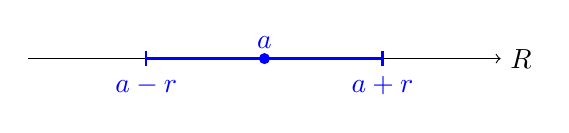
\begin{tikzpicture}
    \draw[->] (-3,0) -- (3,0) node[right] {$\mathbb{R}$};
    \draw[thick, blue] (-1.5,0) -- (1.5,0);
    \draw[blue, thick] (-1.5, 0.1) -- (-1.5, -0.1) node[below] {$a-r$};
    \draw[blue, thick] (1.5, 0.1) -- (1.5, -0.1) node[below] {$a+r$};
    \fill[blue] (0,0) circle (2pt) node[above] {$a$};
\end{tikzpicture}
\end{figure}

\subsubsection*{ii.}
$$ X = \mathbb{R}^n, \quad d_2(x, y) = \sqrt{\sum_{i=1}^n (x_i - y_i)^2} $$

\begin{proof}
\begin{enumerate}
    \item The square root of a sum of squares is nonnegative and vanishes only if each term is
    zero ($x_i = y_i$).
    \item $(x_i - y_i)^2 = (y_i - x_i)^2$, so that the sum is the same.
    \item The triangle inequality is Minkowski's inequality for sums:
    $\|x - z\|_2 \le \|x - y\|_2 + \|y - z\|_2$.
\end{enumerate}
\end{proof}

Open Ball ($n=2$): It is the interior of an ordinary circle.

\subsubsection*{iii.}
$$ X = \mathbb{R}^n, \quad d_1(x, y) = \sum_{i=1}^n |x_i - y_i| $$

\begin{proof}
Properties 1 and 2 follow from those of the absolute value in each coordinate. For the triangle inequality,
in each component $i$ one has $|x_i - z_i| \le |x_i - y_i| + |y_i - z_i|$; summing over $i$ yields
the inequality for the metric.
\end{proof}

Open Ball ($n=2$): $|x_1 - a_1| + |x_2 - a_2| < r$. It is a square rotated by 45 degrees.
\subsubsection*{iv.}
$$ X = \mathbb{R}^n, \quad d_\infty(x, y) = \max_{1 \le i \le n} |x_i - y_i| $$

\begin{proof}
The maximum of nonnegative values is nonnegative and vanishes only if all of them do, and symmetry is
inherited from the absolute value. For the triangle inequality, let $k$ be the index where the maximum of
$|x_i - z_i|$ is attained; then
$$ d_\infty(x, z) = |x_k - z_k| \le |x_k - y_k| + |y_k - z_k| \le d_\infty(x, y) + d_\infty(y, z), $$
since each term is less than or equal to its respective maximum.
\end{proof}

Open Ball ($n=2$): $\max(|x_1 - a_1|, |x_2 - a_2|) < r$. It is a square with sides parallel to the
axes.

\begin{figure}[H]
\centering
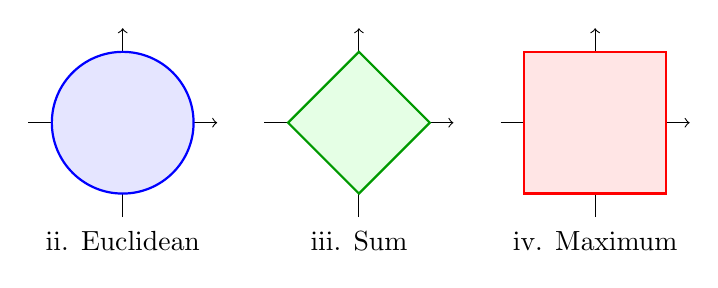
\begin{tikzpicture}[scale=0.6]
    % Euclidean
    \begin{scope}[xshift=-5cm]
        \draw[->] (-2,0) -- (2,0); \draw[->] (0,-2) -- (0,2);
        \draw[thick, blue, fill=blue!10] (0,0) circle (1.5cm);
        \node at (0, -2.5) {ii. Euclidean};
    \end{scope}
    
    % Sum
    \begin{scope}[xshift=0cm]
        \draw[->] (-2,0) -- (2,0); \draw[->] (0,-2) -- (0,2);
        \draw[thick, green!60!black, fill=green!10] (0,1.5) -- (1.5,0) -- (0,-1.5) -- (-1.5,0) --
        cycle;
        \node at (0, -2.5) {iii. Sum};
    \end{scope}

    % Maximum
    \begin{scope}[xshift=5cm]
        \draw[->] (-2,0) -- (2,0); \draw[->] (0,-2) -- (0,2);
        \draw[thick, red, fill=red!10] (-1.5,-1.5) rectangle (1.5,1.5);
        \node at (0, -2.5) {iv. Maximum};
    \end{scope}
\end{tikzpicture}
\end{figure}

\subsubsection*{v.}
$$ X = C([0,1]), \quad d(f, g) = \max_{t \in [0,1]} |f(t) - g(t)| $$

\begin{proof}
Analogous to the maximum metric on $\mathbb{R}^n$, taking the maximum over the continuous interval
$t \in [0,1]$.
\end{proof}

Open Ball: It is a strip or tube of width $2r$ centered at the function $f$.

\begin{figure}[H]
\centering
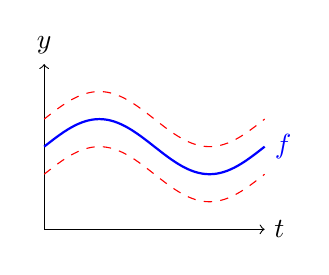
\begin{tikzpicture}[scale=0.7]
    \draw[->] (0,0) -- (4,0) node[right] {$t$};
    \draw[->] (0,0) -- (0,3) node[above] {$y$};
    \draw[thick, blue] (0,1.5) sin (1,2) cos (2,1.5) sin (3,1) cos (4,1.5) node[right] {$f$};
    \draw[dashed, red] (0,2.0) sin (1,2.5) cos (2,2.0) sin (3,1.5) cos (4,2.0);
    \draw[dashed, red] (0,1.0) sin (1,1.5) cos (2,1.0) sin (3,0.5) cos (4,1.0);
\end{tikzpicture}
\end{figure}

\subsubsection*{vi.}
$$ d(x, y) = \begin{cases} 0 & x=y \\ 1 & x \neq y \end{cases} $$

\begin{proof}
Properties 1 and 2 hold by definition. For the triangle inequality, $d(x, z) \le d(x, y) + d(y, z)$:
if $x \neq z$ then $d(x, z) = 1$, and for the sum on the right to be $0$ one would need $x = y$
and $y = z$, which gives $x = z$, a contradiction; hence the right-hand side adds up to at least $1$.
\end{proof}

Open Ball:
\begin{itemize}
    \item If $r \le 1$: $B(x, r) = \{x\}$.
    \item If $r > 1$: $B(x, r) = X$.
\end{itemize}

\subsection*{Exercise 2}

Given fixed $x \in X$ and $r > 0$, prove that the following sets are open.

\subsubsection*{i. The set $\{y \in X : d(x, y) < r\}$}

This exercise has already been solved.

\subsubsection*{ii. The set $A = \{y \in X : d(x, y) > r\}$}

\begin{proof}
Let $y_0 \in A$, that is, $d(x, y_0) = d > r$. A $\delta > 0$ such that
$B(y_0, \delta) \subset A$ must be found. Define
$$ \delta = d(x, y_0) - r, $$
which is positive because $d(x, y_0) > r$. It is shown that $B(y_0, \delta) \subset A$: let
$z \in B(y_0, \delta)$, that is, $d(y_0, z) < \delta$; it must be seen that $d(x, z) > r$. By the
triangle inequality,
$$ d(x, y_0) \le d(x, z) + d(z, y_0) \implies d(x, z) \ge d(x, y_0) - d(z, y_0). $$
Since $d(z, y_0) < \delta$,
$$ d(x, z) > d(x, y_0) - \delta = d(x, y_0) - (d(x, y_0) - r) = r, $$
so that $z \in A$. Hence every point of $A$ has a ball contained in $A$, so that $A$ is
open.
\end{proof}

\subsection*{Exercise 3}

This exercise has already been solved.

\subsection*{Exercise 4}

This exercise has already been solved.

\subsection*{Exercise 5}

Prove the following relations between interior, closure, unions and intersections.

\subsubsection*{i.}
$$ (A \cap B)^\circ = A^\circ \cap B^\circ $$

\begin{proof}
Double inclusion is proved.

\textit{($\subseteq$).} Let $x \in (A \cap B)^\circ$. By definition of interior, there is $r > 0$ with
$$ B(x, r) \subset A \cap B, $$
that is, every $y \in B(x, r)$ satisfies $y \in A$ and $y \in B$. Hence $B(x, r) \subset A$, whence
$x \in A^\circ$, and $B(x, r) \subset B$, whence $x \in B^\circ$; thus $x \in A^\circ \cap B^\circ$.

\textit{($\supseteq$).} Let $x \in A^\circ \cap B^\circ$. There are $r_1, r_2 > 0$ with
$B(x, r_1) \subset A$ and $B(x, r_2) \subset B$. With $r = \min\{r_1, r_2\}$, the ball $B(x, r)$ is
contained in both, so that $B(x, r) \subset A \cap B$ and $x \in (A \cap B)^\circ$.
\end{proof}

\subsubsection*{ii.}
$$ A^\circ \cup B^\circ \subset (A \cup B)^\circ $$

\begin{proof}
Let $x \in A^\circ \cup B^\circ$, that is, $x \in A^\circ$ or $x \in B^\circ$. If $x \in A^\circ$,
there is $r > 0$ with $B(x, r) \subset A \subset A \cup B$, so that $x \in (A \cup B)^\circ$; the case
$x \in B^\circ$ is analogous. In either case $x \in (A \cup B)^\circ$.
\end{proof}

The inclusion may be strict. In the usual $\mathbb{R}$, with $A = [0, 1]$ and $B = [1, 2]$ one has
$A^\circ = (0, 1)$, $B^\circ = (1, 2)$, so that $A^\circ \cup B^\circ = (0, 1) \cup (1, 2)$; on the
other hand $A \cup B = [0, 2]$ has interior $(0, 2)$. The point $1$ is in $(A \cup B)^\circ$ but not
in the union of the interiors.

\subsubsection*{iii.}
$$ \overline{A \cup B} = \overline{A} \cup \overline{B} $$

\begin{proof}
Double inclusion is proved.

\textit{($\supseteq$).} Let $x \in \overline{A} \cup \overline{B}$. If $x \in \overline{A}$, for
every $r > 0$ one has $B(x, r) \cap A \neq \emptyset$, and since $A \subset A \cup B$, also
$B(x, r) \cap (A \cup B) \neq \emptyset$, hence $x \in \overline{A \cup B}$. The case
$x \in \overline{B}$ is analogous.

\textit{($\subseteq$).} By contraposition: suppose $x \notin \overline{A} \cup \overline{B}$;
it must be seen that $x \notin \overline{A \cup B}$. There are $r_1, r_2 > 0$ with $B(x, r_1) \cap A =
\emptyset$ and $B(x, r_2) \cap B = \emptyset$. With $r = \min\{r_1, r_2\}$, the ball $B(x, r)$ is
contained in both, so that $B(x, r) \cap A = \emptyset$ and $B(x, r) \cap B = \emptyset$; therefore
$$ B(x, r) \cap (A \cup B) = (B(x, r) \cap A) \cup (B(x, r) \cap B) = \emptyset, $$
so that $x \notin \overline{A \cup B}$.
\end{proof}

\subsubsection*{iv.}
$$ \overline{A \cap B} \subset \overline{A} \cap \overline{B} $$

\begin{proof}
Let $x \in \overline{A \cap B}$. For every $r > 0$, $B(x, r) \cap (A \cap B) \neq \emptyset$; let
$z$ be in that intersection (it depends on $r$), so that $z \in B(x, r)$, $z \in A$ and $z \in B$.
Then $B(x, r) \cap A \neq \emptyset$ and $B(x, r) \cap B \neq \emptyset$ for every $r$, hence
$x \in \overline{A}$ and $x \in \overline{B}$, that is, $x \in \overline{A} \cap \overline{B}$.
\end{proof}

The inclusion may be strict. In the usual $\mathbb{R}$, with $A = (0, 1)$ and $B = (1, 2)$ one has
$A \cap B = \emptyset$, so that $\overline{A \cap B} = \emptyset$; on the other hand $\overline{A} = [0, 1]$
and $\overline{B} = [1, 2]$, with $\overline{A} \cap \overline{B} = \{1\} \neq \emptyset$.

\subsection*{Exercise 6}

This exercise has already been solved.

\subsection*{Exercise 7}

This exercise has already been solved.

\subsection*{Exercise 8}

This exercise has already been solved.

\subsection*{Exercise 9}

Prove that if $A \subset B$, then the diameter of $A$ is less than or equal to the diameter of $B$, that
is, $d(A) \le d(B)$.

\begin{proof}
The diameter of a nonempty set is $d(A) = \sup \{ d(x, y) : x, y \in A \}$. Consider the
sets of distances
$$ S_A = \{ d(x, y) : x, y \in A \}, \qquad S_B = \{ d(u, v) : u, v \in B \}. $$
Let $r \in S_A$; there are $x_0, y_0 \in A$ with $r = d(x_0, y_0)$. Since $A \subset B$, also
$x_0, y_0 \in B$, so that $r = d(x_0, y_0) \in S_B$. Hence $S_A \subseteq S_B$, and since the supremum is
monotone with respect to inclusion,
$$ d(A) = \sup(S_A) \le \sup(S_B) = d(B). $$
\end{proof}

\subsection*{Exercise 10}

Prove that the set of irrational numbers $\mathbb{R} \setminus \mathbb{Q}$ is not a countable
union of closed sets.

\begin{proof}
Argue by contradiction: suppose that the irrationals $\mathbb{I} = \mathbb{R} \setminus \mathbb{Q}$
are written as a countable union of closed sets,
$$ \mathbb{I} = \bigcup_{n=1}^{\infty} F_n, $$
with each $F_n$ closed in $\mathbb{R}$. Each $F_n \subset \mathbb{I}$, and since the irrationals do not
contain any open interval (the rationals are dense), the interior of each $F_n$ is empty,
$(F_n)^\circ = \emptyset$.

On the other hand, $\mathbb{Q}$ is countable, $\mathbb{Q} = \bigcup_{k=1}^{\infty} \{q_k\}$, and each
$\{q_k\}$ is closed with empty interior. Then
$$ \mathbb{R} = (\mathbb{R} \setminus \mathbb{Q}) \cup \mathbb{Q}
= \left( \bigcup_{n} F_n \right) \cup \left( \bigcup_{k} \{q_k\} \right) $$
is written as a countable union of closed sets with empty interior, that is, $\mathbb{R}$ would be of the
first category. But $\mathbb{R}$ with the usual metric is complete, so that by Baire's
Theorem \ref{teo:baire_v2} it is of the second category, a contradiction. Hence the irrationals are not a countable
union of closed sets.
\end{proof}

\subsection*{Exercise 11}

Given $f \in C([0,1])$, the iterated integrals $f_n$ are defined. Prove that if for each
$x \in [0,1]$ there is an $n \in \mathbb{N}$ such that $f_n(x)=0$, then $f=0$.

\begin{proof}
Let $Z = \{ x \in [0, 1] : f(x) = 0 \}$ be the zero set of $f$. Since $f$ is continuous, $Z$ is
closed (this is seen in the next section); it must be seen that $Z = [0, 1]$. Let $U = Z^\circ$ be the largest
open set where $f$ vanishes; it is proved that $U$ is dense in $[0, 1]$.

Suppose, by contradiction, that $U$ is not dense: there is a nonempty open interval
$(a, b) \subset [0, 1]$ with $(a, b) \cap U = \emptyset$. The closed interval $K = [a, b]$ is a
complete subspace (closed in a complete space). By hypothesis, for each $x \in K$ there is $n$ with
$f_n(x) = 0$, so that with
$$ F_n = \{ x \in K : f_n(x) = 0 \} $$
one has $K = \bigcup_{n=1}^{\infty} F_n$. Since $K$ is complete, by Baire's Theorem
\ref{teo:baire_v2} some $F_N$ has nonempty interior relative to $K$: there is $(c, d) \subset (a, b)$
with $f_N \equiv 0$ on $(c, d)$. Differentiating $N$ times (using $f_k' = f_{k-1}$),
$$ f_N(x) = 0 \implies f_{N-1}(x) = 0 \implies \dots \implies f(x) = 0 \quad \forall x \in (c, d), $$
so that $(c, d) \subset Z^\circ = U$. But $(c, d) \subset (a, b)$, which contradicts
$(a, b) \cap U = \emptyset$.

Hence $U$ is dense in $[0, 1]$. Since $f$ is continuous and vanishes on the dense set $U$, it vanishes on
the whole space: $f(x) = 0$ for every $x \in [0, 1]$.
\end{proof}

\newpage

\section{Compactness, continuity and convergence}

\subsection{Preliminary Definitions}

\begin{definicion}{Open cover}{cubrimiento}
A family $\{U_i\}_{i \in I}$ of open sets is an open cover of $K \subset X$ if
$K \subseteq \bigcup_i U_i$.
\end{definicion}

\begin{definicion}{Finite Subcover}{subcubrimiento}
A cover $\{U_i\}$ has a finite subcover if there are $i_1, \dots, i_n$ with
$K \subseteq U_{i_1} \cup \cdots \cup U_{i_n}$.
\end{definicion}

\subsection{Definition of a Compact Set}

\begin{definicion}{Compactness}{def_compacto}
$K$ is compact if every open cover admits a finite subcover.
\end{definicion}

\subsection{Properties in Metric Spaces}

\begin{proposicion}{Compact Implies Closed}{compacto_es_cerrado}
Every compact set $K$ of a metric space is closed.
\end{proposicion}

\begin{proof}
It is shown that $K^c$ is open. Let $x \notin K$. For each $r > 0$ define
$$ U_r = \{y \in X : d(x, y) > r\}, $$
which is open. For any $z \in K$, $d(x,z) > 0$, so that $z \in U_{d(x,z)/2}$. Hence
$\{U_r\}_{r > 0}$ is an open cover of $K$.

By compactness, there is a finite subcover $U_{r_1}, \dots, U_{r_n}$. Let
$\bar{r} = \min_j r_j > 0$. The $U_{r_j}$ are nested (the smaller $r$, the larger $U_r$), so that
$\bigcup_j U_{r_j} = U_{\bar r}$, and $K \subseteq U_{\bar r}$. That is,
$K \cap \overline{B(x, \bar r)} = \emptyset$. There is a ball around $x$ disjoint from $K$.
\end{proof}

\begin{proposicion}{Compact Implies Bounded}{compacto_es_acotado}
Every compact set $K$ is bounded (it lives inside a ball).
\end{proposicion}

\begin{proof}
Let $x_0 \in K$. The family $\{B(x_0, n)\}_{n \in \mathbb{N}}$ is an open cover of $K$
(because every point is at finite distance from $x_0$). By compactness there is a finite subcover;
taking $N$ the maximum of the radii, $K \subseteq B(x_0, N)$.
\end{proof}

\subsection{Relation to Closed Sets}

\begin{proposicion}{Closed inside Compact}{cerrado_en_compacto}
If $K$ is compact and $F \subset K$ is closed, $F$ is compact.
\end{proposicion}

\begin{proof}
Given an open cover $\{U_i\}$ of $F$, adding the open set $F^c$ yields a
cover of $K$. By compactness a finite one $U_{i_1}, \dots, U_{i_n}, F^c$ is extracted; since
$F \cap F^c = \emptyset$, the $U_{i_j}$ suffice to cover $F$.
\end{proof}

\obs In $\mathbb{R}^n$ with the usual metric the converse holds: compact $\iff$ closed and
bounded. In general it does not. For example, an infinite set with the discrete metric is closed and
bounded (diameter 1) but the cover by balls of radius $1/2$ (each one is a point) does not admit a
finite subcover.


\subsection{Sequential Compactness}

\begin{definicion}{Sequential Compactness}{secuencial_compacto}
$K$ is sequentially compact if every sequence in $K$ admits a subsequence converging to a
point of $K$.
\end{definicion}

\subsection{Totally Bounded Sets}

\begin{definicion}{Totally Bounded}{totalmente_acotado}
$K$ is totally bounded if for every $\epsilon > 0$ there are $x_1, \dots, x_n \in K$ with
$K \subseteq \bigcup_i B(x_i, \epsilon)$. These centers form an $\epsilon$-net.
\end{definicion}

\subsubsection{Relation between Bounded and Totally Bounded}

\begin{proposicion}{Totally Bounded Implies Bounded}{tot_acot_implica_acot}
Totally bounded $\implies$ bounded.
\end{proposicion}

\begin{proof}
Take $\epsilon = 1$ and centers $x_1, \dots, x_n$. Let $M = \max_i d(x_1, x_i)$.
For $z \in K$ there is $k$ with $d(z, x_k) < 1$,
so that $d(z, x_1) \le d(z, x_k) + d(x_k, x_1) < 1 + M$.
Hence $K \subseteq B(x_1, M+1)$.
\end{proof}

\begin{proposicion}{Sequentially Compact Implies Totally Bounded}{sec_comp_tot_acot}
Sequentially compact $\implies$ totally bounded.
\end{proposicion}

\begin{proof}
Argue by contradiction: if it were not totally bounded, there would be $\epsilon > 0$ such that no
finite $\epsilon$-net covers $K$.
Construct $(x_n)$ as follows: $x_1 \in K$ arbitrary; given $x_1, \dots, x_n$,
since the balls $B(x_i, \epsilon)$ do not cover $K$, take $x_{n+1}$ outside them.
By construction $d(x_n, x_m) \ge \epsilon$ for $n \ne m$,
so that no subsequence of $(x_n)$ can be Cauchy, and then none converges.
This contradicts sequential compactness.
\end{proof}

\subsection{Lebesgue Number Lemma}

\begin{proposicion}{Lebesgue's Lemma}{lema_lebesgue}
If $K$ is sequentially compact and $\{U_i\}$ is an open cover of $K$, there is $\eta > 0$ (the
Lebesgue number) such that every ball $B(x, \eta)$ with $x \in K$ fits in some $U_i$.
\end{proposicion}

\begin{proof}
Argue by contradiction: if no such $\eta$ exists, for each $n$ there is $x_n \in K$ with $B(x_n, 1/n)$ not contained
in any $U_i$. By sequential compactness $(x_n)$ has a subsequence $x_{n_k} \to x \in K$. Since
$\{U_i\}$ covers $K$, there is $U_{i_0}$ with $x \in U_{i_0}$, and there is $r > 0$ with
$B(x, r) \subseteq U_{i_0}$. Choosing $k$ large with $d(x_{n_k}, x) < r/2$ and $1/n_k < r/2$, by the
triangle inequality $B(x_{n_k}, 1/n_k) \subseteq B(x, r) \subseteq U_{i_0}$. Contradiction.
\end{proof}

\subsection{Equivalence of Compactness}

\begin{teorema}{Equivalence Theorem}{equiv_compacidad}
$K$ is compact if and only if it is sequentially compact.
\end{teorema}

\begin{proof}
Both implications are proved.

\textit{($\Rightarrow$)} Let $(x_n) \subset K$.
If the set of values $S = \{x_n\}$ is finite, some value is repeated infinitely often
and a constant subsequence is obtained.
If $S$ is infinite, it is shown that it has an accumulation point in $K$
(which then gives the subsequence by the characterization \ref{prop:acumulacion_sucesiones}).
Argue by contradiction: if it did not have one, each $z \in K$ would have $r_z > 0$ with
$B(z, r_z) \cap S \subseteq \{z\}$.
The family $\{B(z, r_z)\}_{z \in K}$ covers $K$; by compactness a
finite subcover $B(z_1, r_{z_1}), \dots, B(z_m, r_{z_m})$ is extracted.
Then $S$ is covered and has at most $m$ elements, a contradiction.

\textit{($\Leftarrow$)} Let $\{U_i\}$ be an open cover.
By Lebesgue there is $\eta > 0$ such that every ball of radius $\eta$ fits in some $U_i$;
being totally bounded, $K$ is covered by finitely many $B(x_j, \eta)$, $j = 1, \dots, n$.
Take $i_j$ with $B(x_j, \eta) \subseteq U_{i_j}$, and $K \subseteq \bigcup_j U_{i_j}$.
\end{proof}

\subsection{Metric Characterization of Compactness}

\begin{teorema}{Compactness, Total Boundedness and Completeness}{carac_metrica_compacidad}
$K$ is compact if and only if it is totally bounded and complete.
\end{teorema}

\begin{proof}
Both implications are proved.

\textit{($\Rightarrow$)} It was already seen that sequentially compact $\implies$ totally bounded. For
completeness, a Cauchy sequence in $K$ has a convergent subsequence (sequential
compactness), and a Cauchy sequence with a convergent subsequence converges to the same limit.

\textit{($\Leftarrow$)} Let $(x_n) \subset K$; a convergent subsequence is sought. Diagonalization
argument:
\begin{itemize}
    \item \textit{Step 1.} $K$ is covered by finitely many balls of radius 1. One of them, $B_1$,
    contains infinitely many terms of $(x_n)$. Let $(x_n^{(1)})$ be that subsequence.
    \item \textit{Step $k$.} The sequence $(x_n^{(k-1)})$ is already available. Since $K$ is covered by finitely many balls of
    radius $1/k$, some $B_k$ contains infinitely many terms of $(x_n^{(k-1)})$; let $(x_n^{(k)})$ be the
    corresponding subsequence.
\end{itemize}
Define the \emph{diagonal} $y_k = x_k^{(k)}$. It is a subsequence of $(x_n)$ (the indices are
increasing because each $(x_n^{(k)})$ is a subsequence of the previous one).

$(y_k)$ is Cauchy: for $j, \ell \ge N$, $y_j$ and $y_\ell$ are both terms of $(x_n^{(N)})$
(because the subsequences are nested), and therefore they live in $B_N$, which has radius $1/N$. Thus
$d(y_j, y_\ell) \le 2/N$. By completeness, $(y_k)$ converges to a point of $K$.
\end{proof}

\subsection{Heine-Borel Theorem}

\begin{teorema}{Heine-Borel}{heine_borel}
$K \subset \mathbb{R}^n$ is compact if and only if it is closed and bounded.
\end{teorema}

\begin{proof}
Both implications are proved.

\textit{($\Rightarrow$)} Already seen in general.

\textit{($\Leftarrow$)} If $K$ is bounded, $K \subset [-M, M]^n$ for some $M$.
Since closed in compact is compact (\ref{prop:cerrado_en_compacto}), it suffices to see that
$C = [-M, M]^n$ is compact.
It is complete (closed in $\mathbb{R}^n$, which is complete) and totally bounded:
given $\epsilon > 0$, in each coordinate $[-M, M]$ there is a finite $\epsilon/n$-net
$\{a_1, \dots, a_p\}$; the product $\{a_1, \dots, a_p\}^n$ is an $\epsilon$-net for $C$
(changing coordinate by coordinate with the triangle inequality,
$d(x, a) \le \sum_i |x_i - a_{k_i}| < \epsilon$).
\end{proof}

\subsection{Continuity in Metric Spaces}

\begin{definicion}{Continuous Function}{def_continuidad}
$f: X \to Y$ is \textbf{continuous} at $a \in X$ if for every $\epsilon > 0$ there is $\delta > 0$ with
$f(B_X(a, \delta)) \subseteq B_Y(f(a), \epsilon)$. $f$ is continuous if it is so at every point.
\end{definicion}

\subsection{Equivalent Forms of Continuity}

\begin{teorema}{Characterizations of Continuity}{equiv_continuidad}
For $f: X \to Y$ the following are equivalent:
\begin{enumerate}
    \item[i)] $f$ is continuous.
    \item[ii)] $f^{-1}(U)$ is open in $X$ for every $U$ open in $Y$.
    \item[iii)] $x_n \to x \implies f(x_n) \to f(x)$.
\end{enumerate}
\end{teorema}

\begin{proof}
The chain $(i) \Rightarrow (ii) \Rightarrow (iii) \Rightarrow (i)$ is proved.

\textit{(i) $\Rightarrow$ (ii):} Let $U$ be open and $a \in f^{-1}(U)$. Since $U$ is open, there is
$\epsilon > 0$ with $B(f(a), \epsilon) \subset U$; by continuity there is $\delta$ with
$f(B(a, \delta)) \subset B(f(a), \epsilon) \subset U$, so that $B(a, \delta) \subset f^{-1}(U)$.

\textit{(ii) $\Rightarrow$ (iii):} If $x_n \to x$ and $\epsilon > 0$, $V = B(f(x), \epsilon)$ is
open and $f^{-1}(V)$ is open with $x \in f^{-1}(V)$. There is $r > 0$ with $B(x, r) \subset f^{-1}(V)$;
for large $n$, $x_n \in B(x, r)$ and $f(x_n) \in V$.

\textit{(iii) $\Rightarrow$ (i):} By contraposition. If $f$ is not continuous at $a$, there is
$\epsilon > 0$ such that for each $\delta = 1/n$ there is $x_n$ with $d(x_n, a) < 1/n$ but
$d(f(x_n), f(a)) \ge \epsilon$. Then $x_n \to a$ and $f(x_n) \not\to f(a)$.
\end{proof}

\subsection{Continuous Functions and Compactness}

\begin{teorema}{Preservation of Compactness}{preservacion_compacidad}
If $f: X \to Y$ is continuous and $K \subset X$ is compact, $f(K)$ is compact.
\end{teorema}

\begin{proof}
Given an open cover $\{U_i\}$ of $f(K)$, the preimages $V_i = f^{-1}(U_i)$ are open
and cover $K$. By compactness, there is a finite subcover $V_{i_1}, \dots, V_{i_n}$; then
$U_{i_1}, \dots, U_{i_n}$ cover $f(K)$.
\end{proof}

\subsection{Weierstrass Theorem}

\begin{corolario}{Existence of Maximum and Minimum}{weierstrass}
If $K$ is compact and $f: K \to \mathbb{R}$ is continuous, $f$ attains a maximum and a minimum on $K$.
\end{corolario}

\begin{proof}
$f(K)$ is compact in $\mathbb{R}$, so that it is closed and bounded (Heine-Borel
\ref{teo:heine_borel}). Closed and bounded
implies that the supremum and infimum exist and are in $f(K)$ (a closed set contains its limit
points, in particular its extremes). Hence there are $x_{\max}, x_{\min} \in K$ with
$f(x_{\max}) = \sup$ and $f(x_{\min}) = \inf$.
\end{proof}

\subsection{Uniform Continuity}

Ordinary continuity is local (at a point $a$). Uniform continuity is global: it requires a uniform
control over the whole domain at once.

\subsubsection{Motivation: Dependence on the Point}

$f(x) = 1/x$ on $(0, \infty)$ is continuous at every point. Given $a > 0$ and $\epsilon > 0$,
$$ \left|\frac{1}{x} - \frac{1}{a}\right| = \frac{|x-a|}{xa}. $$
Bounding $x > a/2$, one gets $\frac{|x-a|}{xa} < \frac{2}{a^2}|x-a|$, so that
$\delta \approx a^2 \epsilon / 2$.

The $\delta$ depends on $a$: as $a \to 0$, $\delta$ becomes arbitrarily small. There is no
single $\delta$ that works on the whole domain.

\textit{Consequence.} This lack of uniformity breaks the preservation of Cauchy sequences. The
sequence $x_n = 1/n$ is Cauchy in $(0, \infty)$ but $f(x_n) = n$ is not.

\subsection{Definition of Uniform Continuity}

\begin{definicion}{Uniform Continuity}{def_cont_uniforme}
$f: X \to Y$ is \textbf{uniformly continuous} if for every $\epsilon > 0$ there is $\delta > 0$ such that for
all $x, y \in X$,
$$ d_X(x, y) < \delta \implies d_Y(f(x), f(y)) < \epsilon. $$
\end{definicion}

The difference lies in the order of the quantifiers: in pointwise continuity, $\delta$ is chosen
after fixing $x$; in uniform continuity, $\delta$ is chosen beforehand and works for all points.

\begin{ejemplo}{Lipschitz Functions}{ej_lipschitz}
$f(x) = mx + b$ is uniformly continuous: $|f(x) - f(y)| = |m||x-y|$, so that
$\delta = \epsilon/|m|$ suffices for every pair of points.
\end{ejemplo}

\subsection{Heine-Cantor Theorem}

\begin{teorema}{Continuity on Compact Sets}{heine_cantor}
If $X$ is compact and $f: X \to Y$ is continuous, then $f$ is uniformly continuous.
\end{teorema}

\begin{proof}
Let $\epsilon > 0$. By continuity, for each $x \in X$ there is $\delta_x > 0$ with
$f(B(x, 2\delta_x)) \subseteq B(f(x), \epsilon/2)$ (a doubled radius is taken in order to use the triangle inequality
later). The $B(x, \delta_x)$ cover $X$; by compactness there is a finite subcover
$B(x_1, \delta_{x_1}), \dots, B(x_n, \delta_{x_n})$. Take $\delta = \min_k \delta_{x_k} > 0$.

If $d(x, y) < \delta$, there is $k$ with $x \in B(x_k, \delta_{x_k})$, and by the triangle inequality
$d(y, x_k) < \delta + \delta_{x_k} \le 2\delta_{x_k}$. Both are in $B(x_k, 2\delta_{x_k})$,
so that $f(x), f(y) \in B(f(x_k), \epsilon/2)$ and
$$ d(f(x), f(y)) \le d(f(x), f(x_k)) + d(f(x_k), f(y)) < \epsilon. $$
\end{proof}

\subsection{Basic properties}

\begin{proposicion}{Relation to Pointwise Continuity}{unif_implica_cont}
Uniformly continuous $\implies$ continuous at every point.
\end{proposicion}

\begin{proof}
Fixing $y = a$ in the definition of uniform continuity recovers continuity at $a$.
\end{proof}

\begin{proposicion}{Preservation of Cauchy Sequences}{cauchy_preservation}
If $f$ is uniformly continuous and $(x_n)$ is Cauchy, $(f(x_n))$ is also Cauchy.
\end{proposicion}

\begin{proof}
Given $\epsilon > 0$, take $\delta$ from uniform continuity and $n_0$ such that
$d(x_n, x_m) < \delta$ for $n, m \ge n_0$. Then $d(f(x_n), f(x_m)) < \epsilon$.
\end{proof}

\subsection{Contractions}

\begin{definicion}{Contraction}{def_contraccion}
$f: X \to X$ is a \textbf{contraction} if there is $\lambda \in [0, 1)$ with
$d(f(x), f(y)) \le \lambda\, d(x, y)$ for all $x, y$.
\end{definicion}

\subsection{Banach Fixed-Point Theorem}

\begin{teorema}{Banach Fixed Point}{banach_fixed_point}
Let $X$ be a complete metric space and $f: X \to X$ a contraction. Then $f$ has a unique fixed
point, and for any $x_0 \in X$ the iteration $x_{n+1} = f(x_n)$ converges to it.
\end{teorema}

\begin{proof}
\textit{Existence.} With $x_0$ fixed, let $x_{n+1} = f(x_n)$. By induction,
$$ d(x_{n+1}, x_n) \le \lambda^n d(x_1, x_0). $$
By the triangle inequality and the geometric sum,
$$ d(x_{n+p}, x_n) \le \sum_{j=0}^{p-1} \lambda^{n+j} d(x_1, x_0) \le \frac{\lambda^n}{1-\lambda}
d(x_1, x_0) \xrightarrow{n \to \infty} 0. $$
Hence $(x_n)$ is Cauchy. By completeness it converges to some $x$. Since $f$ is continuous
(Lipschitz), $f(x) = \lim f(x_n) = \lim x_{n+1} = x$.

\textit{Uniqueness.} If $f(x) = x$ and $f(y) = y$, $d(x, y) = d(f(x), f(y)) \le \lambda d(x, y)$. Since
$1 - \lambda > 0$, $d(x, y) = 0$.
\end{proof}

\subsection{Other classical fixed-point theorems}

\begin{teorema}{Brouwer's Theorem}{teorema_brouwer}
Every continuous map from a closed ball of a Euclidean space into itself admits a fixed
point.
\end{teorema}

\begin{teorema}{Schauder's Theorem}{teorema_shauder}
Every continuous map from a nonempty compact convex set K of a Banach space into K admits a
fixed point.
\end{teorema}

\begin{teorema}{Kakutani's Theorem}{teorema_kakutani}
It generalizes Brouwer to functions that return sets instead of points (correspondences).
If $F: K \to K$ assigns to each point a closed convex subset, and satisfies a certain
continuity property (upper hemicontinuity), then there is a point $x$ such that $x \in F(x)$.
\end{teorema}

\subsection{Failure of Brouwer in Infinite Dimension}

One might think that Brouwer's theorem holds in any normed vector space, that is,
that every continuous function from the closed unit ball (convex, closed and bounded) into itself has a
fixed point. This is false in infinite dimension.

The problem lies in the fact that, in infinite dimension, the closed and bounded ball is not compact.

\begin{ejemplo}{Counterexample in the Sequence Space $\ell_2$}{contraejemplo_brouwer}
Consider the space of square-summable sequences $\ell_2$, the closed unit ball
$\overline{B}(0, 1)$ and the function $f: \overline{B}(0, 1) \to \overline{B}(0, 1)$ given by
$$ f(x_1, x_2, x_3, \dots) = \left( \sqrt{1 - \|x\|^2}, x_1, x_2, \dots \right). $$
\begin{enumerate}
    \item \textit{It is well defined.} The norm of the image is always $1$:
    $$ \|f(x)\|^2 = (\sqrt{1 - \|x\|^2})^2 + x_1^2 + x_2^2 + \dots = 1 - \|x\|^2 + \|x\|^2 = 1, $$
    so that the image falls in the ball (in fact, on the sphere).
    \item \textit{It is continuous.} Its components are.
    \item \textit{It has no fixed point.} By contradiction: suppose $f(x) = x$. Then
    $\|x\| = \|f(x)\| = 1$, and
    equating the first coordinate, $x_1 = \sqrt{1 - \|x\|^2} = 0$; equating the second,
    $x_2 = x_1 = 0$, and inductively $x_n = 0$ for every $n$. Hence $x = 0$, whose norm is $0$, which
    contradicts $\|x\| = 1$. Therefore there is no fixed point: $f$ moves every point.
\end{enumerate}
\end{ejemplo}

\subsection{Homeomorphisms}

\begin{definicion}{Homeomorphism}{def_homeomorfismo}
A function $f: X \to Y$ is a \textbf{homeomorphism} if it satisfies three conditions:
\begin{enumerate}
    \item $f$ is bijective.
    \item $f$ is continuous.
    \item Its inverse $f^{-1}: Y \to X$ is also continuous.
\end{enumerate}
\end{definicion}

\begin{proposicion}{Properties of Homeomorphisms}{prop_homeo}
Homeomorphisms preserve all topological properties. If $f$ is a homeomorphism:
\begin{itemize}
    \item $U$ is open in $X \iff f(U)$ is open in $Y$.
    \item $F$ is closed in $X \iff f(F)$ is closed in $Y$.
    \item $K$ is compact in $X \iff f(K)$ is compact in $Y$.
\end{itemize}
\end{proposicion}

\begin{teorema}{Homeomorphism on Compact Sets}{homeo_compacto}
Let $(X, d_X)$ be a compact metric space and $(Y, d_Y)$ any metric space.
If $f: X \to Y$ is a continuous bijective function, then $f$ is a homeomorphism.
(That is, $f^{-1}: Y \to X$ is automatically continuous).
\end{teorema}

\begin{proof}
Since $f$ is already bijective and continuous, it suffices to prove that its inverse $f^{-1}$ is continuous. A function
is continuous if and only if the preimage of every closed set is closed; applied to $f^{-1}$,
$$ f^{-1} \text{ is continuous } \iff \forall F \subset X \text{ closed}, \ (f^{-1})^{-1}(F)
\text{ is closed in } Y. $$
Since the preimage under the inverse is the direct image, $(f^{-1})^{-1}(F) = f(F)$, the goal
reduces to seeing that $f$ is closed. Let $F \subset X$ be closed:
\begin{enumerate}
    \item being closed in the compact $X$, $F$ is compact;
    \item since $f$ is continuous, $f(F)$ is compact in $Y$;
    \item in every metric space a compact set is closed, so that $f(F)$ is closed in $Y$.
\end{enumerate}
Hence $f$ maps closed sets to closed sets, $f^{-1}$ is continuous and $f$ is a homeomorphism.
\end{proof}

\subsection{Types of Convergence}

There are two main ways in which a sequence of functions can approach a limit function
$f$.

\begin{definicion}{Pointwise Convergence}{conv_puntual}
$(f_n)$ \textbf{converges pointwise} to $f$ if for each fixed $x \in K$ the numerical sequence
$(f_n(x))$ converges to $f(x)$.
$$ \forall x \in K, \quad \lim_{n \to \infty} f_n(x) = f(x) $$
In terms of $\epsilon$: For every $\epsilon > 0$ and every $x$, there is an $n_0$ (depending on
$\epsilon$ and on $x$) such that $n \ge n_0 \implies |f_n(x) - f(x)| < \epsilon$.
\end{definicion}

Pointwise convergence is weak because $n_0$ can grow without bound as $x$ varies. To correct
this, uniform convergence is introduced.

\begin{definicion}{Uniform Convergence}{conv_uniforme}
$(f_n)$ \textbf{converges uniformly} to $f$ if the maximum distance between the functions tends
to zero.
$$ \lim_{n \to \infty} \left( \sup_{x \in K} |f_n(x) - f(x)| \right) = 0 $$
In terms of $\epsilon$: For every $\epsilon > 0$, there is an $n_0$ (depending only on
$\epsilon$, not on $x$) such that for every $n \ge n_0$ and every $x \in K$:
$$ |f_n(x) - f(x)| < \epsilon $$
\end{definicion}

\subsection{The Space C(K) and its Completeness}

$C(K)$ is the set of continuous functions $f: K \to \mathbb{R}$ with $K$ compact, equipped
with the supremum norm $d(f, g) = \max_{x \in K} |f(x) - g(x)|$. Converging in this metric is
exactly converging uniformly.

\begin{teorema}{Completeness of $C(K)$}{ck_completo}
$(C(K), d_\infty)$ is complete: every Cauchy sequence converges uniformly to a continuous
function.
\end{teorema}

\begin{proof}
Let $(f_n)$ be Cauchy in $C(K)$.

\textit{Pointwise limit.} For each $x$, $|f_n(x) - f_m(x)| \le d_\infty(f_n, f_m)$ and $(f_n(x))$ is
Cauchy in $\mathbb{R}$. Since $\mathbb{R}$ is complete, define $f(x) = \lim_n f_n(x)$.

\textit{Uniform convergence.} Being Cauchy, there is $N$ such that $|f_n(x) - f_m(x)| < \epsilon$
for every $x$ and every $n, m \ge N$. Fixing $n$ and letting $m \to \infty$,
$|f_n(x) - f(x)| \le \epsilon$ for every $x$.

\textit{Continuity of the limit.} By the $3\epsilon$ argument: given $a$ and $\epsilon > 0$,
choose $n$ large so that $|f(x) - f_n(x)| < \epsilon/3$ uniformly; then use the
continuity of $f_n$ to obtain $\delta$ with $|f_n(x) - f_n(a)| < \epsilon/3$ when
$d(x, a) < \delta$. By the triangle
inequality,
$$ |f(x) - f(a)| \le |f(x) - f_n(x)| + |f_n(x) - f_n(a)| + |f_n(a) - f(a)| < \epsilon. $$
\end{proof}

\newpage

\subsection{Solved exercises}

\subsection*{Exercise 1}

Prove the implications and give counterexamples.

\subsubsection*{i. Compact $\implies$ Totally Bounded}
This implication has already been proved.

Counterexample: a set can be totally bounded but not compact. Consider the open
interval $(0, 1)$ with the usual metric.
\begin{itemize}
    \item \textit{Totally bounded.} For any $\epsilon$ it is covered by finitely many intervals
    of length $\epsilon$.
    \item \textit{Not compact.} The open cover $\{(1/n, 1)\}_{n \in \mathbb{N}}$ has no
    finite subcover (it fails because it is not complete).
\end{itemize}

\subsubsection*{ii. Totally Bounded $\implies$ Bounded}
This implication has already been proved.

Counterexample: a set can be bounded but not totally bounded. Consider an infinite
set $X$ with the discrete metric.
\begin{itemize}
    \item \textit{Bounded.} The whole set fits in the ball $B(x, 2)$, since the maximum distance is
    $1$.
    \item \textit{Not totally bounded.} For $\epsilon = 1/2$, the balls are individual points
    $\{x\}$, and infinitely many would be needed to cover the set.
\end{itemize}

\subsection*{Exercise 2}

Let $K = \{0\} \cup \{ \frac{1}{n} : n \in \mathbb{N} \} \subset \mathbb{R}$. Prove by definition
that $K$ is compact.

\begin{proof}
Let $\{U_i\}_{i \in I}$ be an open cover of $K$. Since $0 \in K$, there is $i_0$ with $0 \in U_{i_0}$,
and being open there is $r > 0$ with $(-r, r) = B(0, r) \subseteq U_{i_0}$. Since $1/n \to 0$, there is
$N$ such that $1/n < r$ for every $n \ge N$, so that the tail $\{1/n : n \ge N\}$ lies in $U_{i_0}$.
The finitely many points $1, 1/2, \dots, 1/(N-1)$ remain; for each $1/k$ choose an open set $U_{i_k}$ that
contains it. Then
$$ \{ U_{i_0}, U_{i_1}, \dots, U_{i_{N-1}} \} $$
is a finite subcover of $K$. Hence $K$ is compact.
\end{proof}

\subsection*{Exercise 3}

Prove that if a metric space (or subset) is totally bounded, then it is separable.
(As a corollary, every compact metric space is separable).

\begin{proof}
Let $K$ be totally bounded; a countable dense $D \subset K$ is sought.

\textit{Construction of $D$.} For each $n \in \mathbb{N}$, with radius $\epsilon_n = 1/n$,
total boundedness gives a finite net $F_n = \{x_{n,1}, \dots, x_{n,k_n}\} \subset K$ with
$$ K \subseteq \bigcup_{j=1}^{k_n} B\!\left(x_{n,j}, \tfrac{1}{n}\right). $$
Define $D = \bigcup_{n=1}^{\infty} F_n$.

\textit{Countability.} $D$ is a countable union of finite sets, hence it is countable.

\textit{Density.} $D$ is dense if and only if it meets every nonempty open set of $K$. Let $U$ be a nonempty
open set and $x \in U$, with $B(x, r) \subseteq U$. By the Archimedean Property \ref{prop:arquimediana}
there is $N$ with $1/N < r$.
The net $F_N$ covers $K$ with balls of radius $1/N$, so that there is $z \in F_N$ with $d(x, z) < 1/N < r$,
whence $z \in B(x, r) \subseteq U$. Since $z \in D \cap U$, one has $D \cap U \neq \emptyset$. Hence
$D$ is dense in $K$.
\end{proof}

\subsection*{Exercise 4}

Given a family of closed sets $(F_{\alpha})$ such that one of them, $F_{\alpha'}$, is compact,
prove that $K = \bigcap_{\alpha} F_{\alpha}$ is compact. Can it be empty?

\begin{proof}
An arbitrary intersection of closed sets is closed, so that $K = \bigcap_\alpha F_\alpha$ is closed.
Moreover $K \subseteq F_{\alpha'}$, so that $K$ is a closed set contained in the compact set
$F_{\alpha'}$; by Proposition \ref{prop:cerrado_en_compacto}, $K$ is compact.
\end{proof}

The intersection can be empty, and the empty set is compact. For example, in $\mathbb{R}$, with
$F_1 = [0, 1]$ (compact) and $F_2 = [2, 3]$ (closed), one has $F_1 \cap F_2 = \emptyset$.

\subsection*{Exercise 5}

Prove that $X$ is compact $\iff$ for every decreasing sequence $(F_n)$ of nonempty closed sets,
$\bigcap_{n=1}^{\infty} F_n \neq \emptyset$.

\begin{proof}
\textit{($\Rightarrow$).} Argue by contradiction: suppose there is a sequence $(F_n)$ of nonempty
decreasing closed sets with $\bigcap_{n=1}^{\infty} F_n = \emptyset$. With $U_n = F_n^c$ (open), by
De Morgan
$$ \bigcup_{n=1}^{\infty} U_n = \left( \bigcap_{n=1}^{\infty} F_n \right)^c = X, $$
so that $\{U_n\}$ is an open cover of $X$. By compactness there is a finite subcover
$U_{n_1}, \dots, U_{n_k}$; since $(F_n)$ decreases, $(U_n)$ increases, and with $N = \max\{n_1, \dots, n_k\}$ one
has $\bigcup_j U_{n_j} = U_N = X$. Taking complements, $F_N = \emptyset$, which contradicts
the $F_n$ being nonempty.

\textit{($\Leftarrow$).} By contraposition: suppose that $X$ is not compact. In a metric
space this gives a countable cover $\{U_n\}$ with no finite subcover. With
$A_n = U_1 \cup \dots \cup U_n$ define $F_n = X \setminus A_n$. Each $F_n$ is closed (complement
of a finite union of open sets), the sequence decreases ($A_n$ increases, so that $F_{n+1} \subset F_n$) and it is
nonempty (if some $A_n = X$, then $U_1, \dots, U_n$ would be a finite subcover). However,
$$ \bigcap_{n=1}^{\infty} F_n = X \setminus \bigcup_{n=1}^{\infty} A_n = X \setminus
\bigcup_{n=1}^{\infty} U_n = X \setminus X = \emptyset. $$
Thus a decreasing sequence of nonempty closed sets with empty intersection is constructed.
\end{proof}

\subsection*{Exercise 6}

The distance between two sets is defined as $d(A, B) = \inf \{ d(x, y) : x \in A, y \in B \}$.

\subsubsection*{i.}
\begin{proposicion}{Positive Distance}{dist_compact_closed}
If $A$ is compact and $B$ is closed with $A \cap B = \emptyset$, then $d(A, B) > 0$.
\end{proposicion}

\begin{proof}
Argue by contradiction: suppose $d(A, B) = 0$. By definition of infimum, for each $n$ there are
$x_n \in A$ and $y_n \in B$ with $d(x_n, y_n) < 1/n$, so that $d(x_n, y_n) \to 0$. Since $A$ is compact,
it is sequentially compact (\ref{teo:equiv_compacidad}), and $(x_n)$ has a subsequence
$x_{n_k} \to a \in A$. By the
triangle inequality,
$$ d(y_{n_k}, a) \le d(y_{n_k}, x_{n_k}) + d(x_{n_k}, a), $$
where $d(y_{n_k}, x_{n_k}) < 1/n_k \to 0$ and $d(x_{n_k}, a) \to 0$, so that $y_{n_k} \to a$. Since
$B$ is closed, $a \in B$. Then $a \in A \cap B$, which contradicts $A \cap B = \emptyset$. Hence
$d(A, B) > 0$.
\end{proof}

\subsubsection*{ii.}
If $A$ and $B$ are only disjoint closed sets, it may happen that $d(A, B) = 0$. As a counterexample in
$\mathbb{R}^2$, consider the hyperbola and the $x$-axis:
$$ A = \{ (x, y) : xy = 1 \}, \qquad B = \{ (x, y) : y = 0 \}. $$
\begin{itemize}
    \item \textit{Closed.} Both are preimages of closed sets under continuous functions.
    \item \textit{Disjoint.} In $A$ the $y$ coordinate is never $0$ (since $xy = 1$); in $B$ it is always
    $0$.
    \item \textit{Zero distance.} With $a_n = (n, 1/n) \in A$ and $b_n = (n, 0) \in B$,
    $$ d(a_n, b_n) = \sqrt{(n-n)^2 + (1/n)^2} = \frac{1}{n} \to 0, $$
    so that the infimum of the distances is $0$.
\end{itemize}
Without compactness, the sets can approach each other asymptotically without touching.

\subsection*{Exercise 7}

Given compact subsets $A$ and $B$ of $\mathbb{R}^n$, prove that the set
$A - B = \{a - b : a \in A, b \in B\}$ is compact.

\begin{proof}
It must be seen that every sequence in $A - B$ has a subsequence converging to a point of $A - B$.
Let $(z_n) \subset A - B$, with $z_n = a_n - b_n$, $a_n \in A$, $b_n \in B$. Since $A$ is compact, there is
a subsequence $a_{n_k} \to a \in A$. Since $B$ is compact, $(b_{n_k})$ has in turn a
subsequence $b_{n_{k_j}} \to b \in B$. By the algebra of limits in $\mathbb{R}^n$
(\ref{teo:algebra_limites}),
$$ z_{n_{k_j}} = a_{n_{k_j}} - b_{n_{k_j}} \to a - b, $$
and $a - b \in A - B$. Hence $A - B$ is sequentially compact (\ref{teo:equiv_compacidad}), that is, compact.
\end{proof}

\subsection*{Exercise 8}

On the set $c_0$ of sequences of real numbers tending to 0, define the distance
$d(x, y) = \sup_n |x_n - y_n|$.
Prove that the closed unit ball $\overline{B}(0, 1)$ is not sequentially compact.

\begin{proof}
A set is sequentially compact if every sequence in it admits a convergent subsequence.
A sequence in $\overline{B}(0, 1)$ with no convergent subsequences is constructed.

\textit{Construction.} Let $(e^{(n)})$ be the sequence of canonical vectors, with $e^{(n)}$ the sequence
that equals $1$ at position $n$ and $0$ elsewhere.

\textit{Membership.} Each $e^{(n)}$ tends to $0$ (it is eventually zero), so that $e^{(n)} \in c_0$,
and $\|e^{(n)}\|_\infty = \sup_k |e^{(n)}_k| = 1$, so that $e^{(n)} \in \overline{B}(0, 1)$.

\textit{Distance between terms.} For $n \neq m$, the difference $e^{(n)} - e^{(m)}$ equals $1$ at
position $n$, $-1$ at position $m$ and $0$ elsewhere, so that
$$ d(e^{(n)}, e^{(m)}) = \sup_k |e^{(n)}_k - e^{(m)}_k| = 1. $$

\textit{Conclusion.} By contradiction: if $(e^{(n_k)})$ converged, it would be Cauchy, and its terms would be at
distance $< \epsilon$ from each other; but the distance between two distinct terms is always $1$. Hence
no subsequence converges, and $\overline{B}(0, 1)$ is not sequentially compact.
\end{proof}

\subsection*{Exercise 9}

\subsubsection*{i.}
Prove that $f: \mathbb{R} \to \mathbb{R}$ such that $f(x) = x^2$ is continuous, but there is an open set
$G$ such that $f(G)$ is not open.

\begin{proof}
$f(x) = x^2$ is continuous on $\mathbb{R}$. Consider the open set $G = (-1, 1)$; its direct image is
$$ f(G) = \{ x^2 : -1 < x < 1 \} = [0, 1). $$
The point $y = 0 \in f(G)$ is not interior: for every $\epsilon > 0$, the ball
$B(0, \epsilon) = (-\epsilon, \epsilon)$ contains negative numbers, which are not in $[0, 1)$, so
that $(-\epsilon, \epsilon) \not\subset [0, 1)$. Hence $f(G)$ is not open.
\end{proof}

\subsubsection*{ii.}
Prove that $g: \mathbb{R} \to \mathbb{R}$ such that $g(x) = \frac{x^2}{1+x^2}$ is continuous, but
there is a closed set $F$ such that $g(F)$ is not closed.

\begin{proof}
$g$ is continuous as a quotient of polynomials with nonvanishing denominator ($1 + x^2 \ge 1$). Consider
the closed set $F = [0, +\infty)$. At $x = 0$ one has $g(0) = 0$; for $x > 0$ it is strictly increasing, and
$$ \lim_{x \to +\infty} \frac{x^2}{1+x^2} = 1, $$
so that $g(F) = [0, 1)$. The sequence $y_n = g(n) = \frac{n^2}{1+n^2} \in g(F)$ satisfies $y_n \to 1$, so
that $1$ is an accumulation point of $[0, 1)$ but $1 \notin [0, 1)$. Since it is missing a limit
point, $g(F)$ is not closed.
\end{proof}

\subsection*{Exercise 10}

Let $f, g: X \to Y$ be continuous functions.

\subsubsection*{i.}
Prove that $A = \{x \in X : f(x) \neq g(x)\}$ is open.

\begin{proof}
Let $a \in A$, that is, $f(a) \neq g(a)$, with $d(f(a), g(a)) = \epsilon > 0$. With $r = \epsilon/2$,
the balls $B(f(a), r)$ and $B(g(a), r)$ are disjoint. By continuity, there are
$\delta_1, \delta_2 > 0$ with $f(B(a, \delta_1)) \subset B(f(a), r)$ and
$g(B(a, \delta_2)) \subset B(g(a), r)$. With $\delta = \min\{\delta_1, \delta_2\}$, for
$x \in B(a, \delta)$ one has $f(x) \in B(f(a), r)$ and $g(x) \in B(g(a), r)$; since those balls are
disjoint, $f(x) \neq g(x)$ and $x \in A$. Hence $B(a, \delta) \subset A$, and $A$ is open.
\end{proof}

\subsubsection*{ii.}
Deduce that $E = \{x \in X : f(x) = g(x)\}$ is closed.

\begin{proof}
The set $E$ is the complement of $A$: $E = A^c$. Since $A$ is open (previous item), its
complement $E$ is closed.
\end{proof}

\subsubsection*{ii. (Alternative)}

Another proof that $E = \{x \in X : f(x) = g(x)\}$ is closed.

\begin{proof}
Define the auxiliary function $h: X \to \mathbb{R}$, $h(x) = f(x) - g(x)$, which is continuous as a
difference of continuous functions. A point $x$ is in $E$ if and only if $f(x) = g(x)$, that is, $h(x) = 0$, so
that $E = h^{-1}(\{0\})$. Since $\{0\}$ is closed in $\mathbb{R}$ and $h$ is continuous, $E$ is closed.
\end{proof}

\subsubsection*{iii.}
Prove that if $D$ is dense in $X$ and $f(x) = g(x)$ for every $x \in D$, then $f = g$ on all of $X$.

\begin{proof}
Consider $E = \{x \in X : f(x) = g(x)\}$. By hypothesis $D \subseteq E$, and taking closures,
$\overline{D} \subseteq \overline{E}$. Since $D$ is dense, $\overline{D} = X$, and since $E$ is closed
(item ii), $\overline{E} = E$. Hence $X \subseteq E$, that is, $f(x) = g(x)$ for every $x \in X$.
\end{proof}

\subsubsection*{iii. (Alternative)}
Prove that if $D$ is dense in $X$ and $f(x) = g(x)$ for every $x \in D$, then $f = g$ on all of $X$.

\begin{proof}
Let $x \in X$. Since $D$ is dense, $x \in \overline{D}$, so that there is $(d_n) \subset D$ with
$d_n \to x$. By hypothesis $f(d_n) = g(d_n)$ for every $n$, and since $f$ and $g$ are continuous,
$f(d_n) \to f(x)$ and $g(d_n) \to g(x)$. Since the sequences $(f(d_n))$ and $(g(d_n))$ coincide term
by term, their limits are equal: $f(x) = g(x)$. Since $x$ was arbitrary, $f = g$ on $X$.
\end{proof}

\subsection*{Exercise 11}

Let $f: \mathbb{R} \to \mathbb{R}$ be continuous and such that there are $a, b \in \mathbb{R}$ with $f(a) < 0$ and
$f(b) > 0$. Prove that there is a $c \in \mathbb{R}$ such that $f(c) = 0$.

\begin{proof}
Without loss of generality, $a < b$. Define
$$ A = \{ x \in [a, b] : f(x) \le 0 \}. $$
\textit{Existence of the supremum.} Since $f(a) < 0$, $a \in A$, so that $A \neq \emptyset$; and
$A \subseteq [a, b]$, so that $b$ is an upper bound. By the Completeness Axiom
(\ref{teo:axioma_completitud}) there is $c = \sup(A)$, with $a \le c \le b$.

\textit{$f(c) = 0$.} The other two cases are ruled out by continuity.

\textit{Case $f(c) < 0$.} By continuity, there is $\delta > 0$ with $f(x) < 0$ on
$(c - \delta, c + \delta)$. Since $f(b) > 0$, $c < b$, and one can choose $x_0$ with
$c < x_0 < c + \delta$; then $f(x_0) < 0$, so that $x_0 \in A$ with $x_0 > c$, which contradicts
$c$ being an upper bound.

\textit{Case $f(c) > 0$.} By continuity, there is $\delta > 0$ with $f(x) > 0$ on
$(c - \delta, c + \delta)$, so that no point of $(c - \delta, c]$ is in $A$ and every $x \in A$
satisfies $x \le c - \delta$; then $c - \delta < c$ would be an upper bound, against $c$ being the
least.

Hence $f(c) = 0$.
\end{proof}

\subsection*{Exercise 12}

Prove that being bounded, being complete and being Cauchy are not homeomorphic properties (that is, they are not
necessarily preserved by homeomorphisms).

By counterexamples. Consider two classical metric spaces with the usual metric:
\begin{itemize}
    \item $X = (0, 1)$.
    \item $Y = \mathbb{R}$.
\end{itemize}
There is a homeomorphism between them, for example the scaled tangent:
$$ f: (0, 1) \to \mathbb{R}, \quad f(x) = \tan\left( \pi \left( x - \frac{1}{2} \right) \right) $$
This function is bijective, continuous and its inverse is continuous. However, the metric properties
are not preserved.

\subsubsection*{i}
\begin{itemize}
    \item The space $X = (0, 1)$ is bounded (its diameter is 1).
    \item Its homeomorphic image $Y = \mathbb{R}$ is unbounded.
\end{itemize}
Hence, boundedness is not a topological invariant.

\subsubsection*{ii.}
\begin{itemize}
    \item The space $Y = \mathbb{R}$ is complete (every Cauchy sequence converges).
    \item The space $X = (0, 1)$ is not complete.
    \textit{Justification:} The sequence $x_n = \frac{1}{n+1}$ is contained in $(0, 1)$. It is a
    Cauchy sequence (because in $\mathbb{R}$ it converges to 0, so that the terms get close together). However,
    its limit (0) does not belong to the space $(0, 1)$. Therefore, within $X$, the
    sequence does not converge.
\end{itemize}
Since $X \cong Y$ but one is complete and the other is not, completeness is not a topological invariant.

\subsubsection*{iii.}
A homeomorphism can transform a Cauchy sequence into one that is not. Consider the
homeomorphism $g: (0, 1) \to (1, +\infty)$ given by $g(x) = \frac{1}{x}$.

\begin{itemize}
    \item The sequence $x_n = \frac{1}{n}$ (for $n \ge 2$) is in $(0, 1)$ and is Cauchy, since
    $\left| \frac{1}{n} - \frac{1}{m} \right| \to 0$.
    \item Applying $g$, $y_n = g(x_n) = n$.
    \item The image sequence $(2, 3, 4, \dots)$ is not Cauchy, since the distance between consecutive
    terms is always $1$.
\end{itemize}
Hence, being a Cauchy sequence is a property that depends on the specific metric and is not
preserved under homeomorphisms.

\subsection*{Exercise 13}

This exercise has already been solved.

\subsection*{Exercise 14}

Prove uniform continuity in the following cases.

\subsubsection*{i.}
$f: \mathbb{R} \to \mathbb{R}$ such that $f(x) = 2x$.

\begin{proof}
It is Lipschitz: $|f(x) - f(y)| = 2|x - y|$. Given $\epsilon > 0$, with $\delta = \epsilon/2$, if
$|x - y| < \delta$ then $|f(x) - f(y)| = 2|x - y| < \epsilon$. Hence $f$ is uniformly
continuous.
\end{proof}

\subsubsection*{ii.}
$f: [0, \infty) \to \mathbb{R}$ such that $f(x) = \sqrt{x}$.

\begin{proof}
% TODO complete the proof of the uniform continuity of $\sqrt{x}$ on $[0,\infty)$.
\end{proof}

\subsubsection*{iii.}
$f: [0, 1] \to \mathbb{R}$ such that $f(x) = x^2$.

\begin{proof}
$f$ is continuous (polynomial) and the domain $[0, 1]$ is closed and bounded, hence compact in
$\mathbb{R}$. By the Heine-Cantor Theorem \ref{teo:heine_cantor}, $f$ is uniformly continuous.
\end{proof}

\subsubsection*{Counterexample:}
Prove that $f: \mathbb{R} \to \mathbb{R}$ such that $f(x) = x^2$ is not uniformly continuous.

\begin{proof}
By the characterization with sequences: if $f$ were uniformly continuous, it would send sequences with
$|x_n - y_n| \to 0$ to sequences with $|f(x_n) - f(y_n)| \to 0$. With $x_n = n$ and $y_n = n + 1/n$,
$$ |x_n - y_n| = \frac{1}{n} \to 0, $$
but
$$ |f(x_n) - f(y_n)| = \left| n^2 - \left(n + \tfrac{1}{n}\right)^2 \right|
= \left| -2 - \tfrac{1}{n^2} \right| = 2 + \frac{1}{n^2} \to 2 \neq 0. $$
Since the distance between the images does not tend to $0$, $f$ is not uniformly continuous.
\end{proof}

\subsection*{Exercise 15}

Prove that if $f: \mathbb{R} \to \mathbb{R}$ is continuous and $\lim_{|x| \to \infty} f(x) = 0$,
then $f$ is uniformly continuous.

\begin{proof}
Given $\epsilon > 0$, a $\delta$ valid on all of $\mathbb{R}$ must be found.

\textit{Tails.} Since $\lim_{|x| \to \infty} f(x) = 0$, there is $M > 0$ such that $|f(x)| < \epsilon/2$
for $|x| > M$.

\textit{Center.} The interval $K = [-M-1, M+1]$ is compact, so that by the Heine-Cantor Theorem
\ref{teo:heine_cantor} $f$ is uniformly continuous on $K$: there is $\delta_K > 0$ such that
$|x - y| < \delta_K \implies |f(x) - f(y)| < \epsilon$ for $x, y \in K$.

\textit{Choice of $\delta$.} Take $\delta = \min(1, \delta_K)$, and let $x, y \in \mathbb{R}$ with
$|x - y| < \delta$.
\begin{itemize}
    \item If $|x| > M$ and $|y| > M$, then $|f(x) - f(y)| \le |f(x)| + |f(y)| < \epsilon$.
    \item If, for example, $x \in [-M, M]$, since $|x - y| < \delta \le 1$ one has
    $|y| \le |x| + 1 \le M + 1$, so that $x, y \in K$ and, by uniform continuity on $K$,
    $|f(x) - f(y)| < \epsilon$.
\end{itemize}
In all cases $|f(x) - f(y)| < \epsilon$, hence $f$ is uniformly continuous on $\mathbb{R}$.
\end{proof}

\newpage

\section{Classification of Spaces and Convexity}

\begin{definicion}{Hilbert Space}{}
A \textbf{Hilbert} space is a vector space $H$ with an inner product $\langle\cdot, \cdot\rangle$, complete
with respect to the metric induced by $\|x\| = \sqrt{\langle x, x \rangle}$.
\end{definicion}

\begin{definicion}{Banach Space}{}
A \textbf{Banach} space is a normed space $(X, \|\cdot\|)$ complete with respect to $d(x,y) = \|x-y\|$.
\end{definicion}

Every Hilbert space is a Banach space, but not conversely. The following are classical examples of Banach spaces that are not
Hilbert spaces.

\begin{ejemplo}{The Space $\ell^1$}{}
$\ell^1 = \{x = (x_n) : \sum |x_n| < \infty\}$, with norm $\|x\|_1 = \sum |x_n|$.
\end{ejemplo}

\begin{ejemplo}{The Space $\ell^\infty$}{}
$\ell^\infty = \{x = (x_n) : \sup_n |x_n| < \infty\}$, with norm $\|x\|_\infty = \sup_n |x_n|$.
\end{ejemplo}

\begin{definicion}{Fréchet Space}{}
A locally convex, complete topological vector space whose topology is induced by
a translation-invariant metric (typically by a countable family of seminorms).
\end{definicion}

\begin{definicion}{Locally Convex Space}{}
A topological space whose topology is generated by a family of seminorms; or,
equivalently, where the origin has a base of convex neighborhoods.
\end{definicion}

\subsection{Difference between Hilbert and Banach: Parallelogram Law}

\begin{teorema}{Parallelogram Law}{paralelogramo}
The norm of $(X, \|\cdot\|)$ comes from an inner product if and only if for all $x, y \in X$
$$ \|x + y\|^2 + \|x - y\|^2 = 2(\|x\|^2 + \|y\|^2). $$
\end{teorema}

\obs $\ell^1$ and $\ell^\infty$ do not satisfy the parallelogram law: it already fails with the canonical vectors $e_1, e_2$.
That is why they are Banach but not Hilbert.

\obs (Polarization identity). When the parallelogram law holds, the inner product is recovered
from the norm:
$$ \langle x, y \rangle = \tfrac{1}{4}\left(\|x + y\|^2 - \|x - y\|^2\right). $$

\subsection{Convexity and Continuity}

\begin{definicion}{Convex Set}{}
$C$ is \textbf{convex} if $tx + (1-t)y \in C$ for all $x, y \in C$ and $t \in [0,1]$.
\end{definicion}

\begin{proposicion}{Convexity of the Closed Ball}{}
$\overline{B}(0,1) = \{x : \|x\| \le 1\}$ is convex in every normed space.
\end{proposicion}

\begin{proof}
For $x, y$ with $\|x\|, \|y\| \le 1$ and $t \in [0,1]$, by the triangle inequality and homogeneity
$\|tx + (1-t)y\| \le t\|x\| + (1-t)\|y\| \le 1$.
\end{proof}

\subsubsection{Relation to the continuity of addition}
The previous proof depends on the triangle inequality $\|x+y\| \le \|x\| + \|y\|$, which is the same property
that guarantees the continuity of addition $+: X \times X \to X$. Geometrically, the convexity of
the ball says that convex combinations (averages) do not escape the neighborhood. In locally
convex spaces it is explicitly required that the origin have a base of convex neighborhoods so that
the topology interacts well with the linear structure.

\subsection{Relation between sequence spaces and compactness}

\begin{proposicion}{Inclusion of $\ell^1$ in $\ell^\infty$}{}
$\ell^1 \subset \ell^\infty$ with $\|x\|_\infty \le \|x\|_1$.
\end{proposicion}

\begin{proof}
For each $k$, $|x_k| \le \sum_n |x_n| = \|x\|_1$; taking the sup over $k$, $\|x\|_\infty \le \|x\|_1$.
\end{proof}

\begin{ejemplo}{}{}
The unit ball $\overline{B}_{\ell^1}(0,1)$ is not sequentially compact. The canonical vectors
$e^{(n)}$ (a 1 at position $n$, zero elsewhere) satisfy $\|e^{(n)}\|_1 = 1$. But for
$n \ne m$,
$$ \|e^{(n)} - e^{(m)}\|_1 = 2, $$
so that no subsequence is Cauchy and, since $\ell^1$ is complete, none converges.
\end{ejemplo}

\subsection{\texorpdfstring{$L^p$ and $\ell^p$ Spaces}{Lp and lp Spaces}}

The $\ell^1$ and $\ell^\infty$ seen before are the two extremes of a much broader family.

\begin{definicion}{The Space $L^p$}{Lp}
Let $(X, \mathcal{A}, \mu)$ be a measure space and $1 \le p < \infty$. The space $L^p(\mu)$ (or
simply $L^p$) is the set of measurable functions $f: X \to \mathbb{R}$ with
$$ \int_X |f|^p \, d\mu < \infty. $$
To each one is assigned
$$ \|f\|_p = \left( \int_X |f|^p \, d\mu \right)^{1/p}. $$
\end{definicion}

\obs
$\|\cdot\|_p$ is not properly a norm but a seminorm: it satisfies $\|af\|_p = |a|\,\|f\|_p$ and the
triangle inequality (Minkowski, below), but $\|f\|_p = 0$ only says that $f = 0$ almost everywhere, not
everywhere. To make it a norm, one takes the quotient by the relation ``equal almost everywhere''.

\begin{ejemplo}{The Space $\ell^p$ as a Particular Case}{ellp}
If $X = \mathbb{N}$ with the counting measure ($\mu(\{n\}) = 1$ for every $n$), the functions are
sequences $a = (a_n)$ and the integral becomes a sum. This yields
$$ \ell^p = \left\{ a = (a_n)_{n \in \mathbb{N}} : \sum_{n=1}^{\infty} |a_n|^p < \infty \right\},
\qquad \|a\|_p = \left( \sum_{n=1}^{\infty} |a_n|^p \right)^{1/p}. $$
\end{ejemplo}

\begin{proposicion}{Inclusion between $\ell^p$ Spaces}{inclusion_lp}
If $1 \le p_1 < p_2 \le \infty$, then $\ell^{p_1} \subseteq \ell^{p_2}$ and
$\|a\|_{p_2} \le \|a\|_{p_1}$ for every $a \in \ell^{p_1}$.
\end{proposicion}

\begin{proof}
If $a \in \ell^{p_1}$ with $\|a\|_{p_1} = 0$, then $a = 0$ and there is nothing to prove. By
homogeneity one may suppose $\|a\|_{p_1} = 1$. Then $|a_n|^{p_1} \le 1$ for every $n$, in
particular $|a_n| \le 1$. Since $p_2 > p_1$ and $|a_n| \le 1$, one has $|a_n|^{p_2} \le |a_n|^{p_1}$.
Summing,
$$ \|a\|_{p_2}^{p_2} = \sum |a_n|^{p_2} \le \sum |a_n|^{p_1} = \|a\|_{p_1}^{p_1} = 1, $$
so that $\|a\|_{p_2} \le 1 = \|a\|_{p_1}$. For $p_2 = \infty$,
$\|a\|_\infty = \sup_n |a_n| \le 1$.
\end{proof}

\begin{proposicion}{Inclusion in Finite Measure}{inclusion_lp_finita}
If $\mu(X) < \infty$ and $1 \le p_1 < p_2 < \infty$, then $L^{p_2}(\mu) \subseteq L^{p_1}(\mu)$.
\end{proposicion}

\begin{proof}
Let $f \in L^{p_2}$. Split $X$ according to where $|f|$ is large or small: $A = \{|f| \le 1\}$,
$A^c = \{|f| > 1\}$. On $A$, $|f|^{p_1} \le 1$. On $A^c$, $|f|^{p_1} < |f|^{p_2}$ (because $|f| > 1$
and $p_1 < p_2$). Thus,
$$ \int_X |f|^{p_1} d\mu = \int_A |f|^{p_1} d\mu + \int_{A^c} |f|^{p_1} d\mu \le \mu(A) + \int_{A^c}
|f|^{p_2} d\mu \le \mu(X) + \|f\|_{p_2}^{p_2} < \infty. $$
\end{proof}

\obs In infinite measure the inclusion fails in both directions. On $\mathbb{R}$ with Lebesgue measure:
$1/\sqrt{x} \cdot \mathbf{1}_{(0,1)} \in L^1 \setminus L^2$ (since $\int_0^1 x^{-1/2}\,dx = 2$ but $\int_0^1 x^{-1}\,dx = \infty$), and
$1/x \cdot \mathbf{1}_{(1,\infty)} \in L^2 \setminus L^1$. For sequences (counting measure, which is
infinite) the inclusion goes the opposite way from $L^p$ with finite measure: $\ell^{p_1} \subseteq \ell^{p_2}$
when $p_1 < p_2$.

\subsection{Young's Inequality}

\begin{teorema}{Young's Inequality}{young}
Let $p, q \in (1, \infty)$ be conjugate exponents, that is,
$$ \frac{1}{p} + \frac{1}{q} = 1. $$
For every pair $a, b \ge 0$,
$$ ab \le \frac{a^p}{p} + \frac{b^q}{q}. $$
\end{teorema}

\begin{proof}
If $a = 0$ or $b = 0$ the left-hand side is $0$ and the inequality holds. Suppose then
$a, b > 0$. The
exponential function $\exp: \mathbb{R} \to \mathbb{R}$ is convex, so that for every pair of reals
$u, v$ and every $t \in [0, 1]$,
$$ \exp\big(tu + (1-t)v\big) \le t \exp(u) + (1-t)\exp(v). $$
Taking $t = 1/p$, $1 - t = 1/q$, $u = \ln(a^p)$ and $v = \ln(b^q)$ yields
$$ \exp\!\left(\frac{1}{p} \ln(a^p) + \frac{1}{q} \ln(b^q)\right)
\le \frac{1}{p} \exp(\ln(a^p)) + \frac{1}{q} \exp(\ln(b^q)) = \frac{a^p}{p} + \frac{b^q}{q}. $$
On the other hand, the argument of the exponential on the left-hand side is $\ln(a) + \ln(b) =
\ln(ab)$, so that $\exp(\cdot) = ab$. Combining both equalities gives the stated
inequality.
\end{proof}

\obs With $p = q = 2$ the inequality reduces to the inequality between the arithmetic and the
geometric mean: $ab \le \tfrac{a^2 + b^2}{2}$.

\obs Equality is attained if and only if $a^p = b^q$. This follows from equality in the
convexity inequality of the exponential, which holds precisely when $u = v$, that is
$\ln(a^p) = \ln(b^q)$.

\subsection{Hölder's Inequality}

\begin{teorema}{Hölder's Inequality}{holder}
Let $p, q \in (1, \infty)$ be conjugate exponents and $f \in L^p(\mu)$, $g \in L^q(\mu)$. Then
$fg \in L^1(\mu)$ and
$$ \|fg\|_1 \le \|f\|_p \, \|g\|_q. $$
\end{teorema}

\begin{proof}
If $\|f\|_p = 0$ then $f = 0$ almost everywhere, so that $fg = 0$ almost everywhere and
both sides vanish. Analogously if $\|g\|_q = 0$. In what follows suppose
$\|f\|_p, \|g\|_q \in (0, \infty)$.

The normalized case $\|f\|_p = \|g\|_q = 1$ is treated first. Young's inequality
\ref{teo:young} applied
at each point $x \in X$ to the numbers $|f(x)|, |g(x)| \ge 0$ yields
$$ |f(x) g(x)| \le \frac{|f(x)|^p}{p} + \frac{|g(x)|^q}{q}. $$
The measurability of $fg$ follows from that of $f$ and $g$. Integrating the previous inequality,
$$ \int_X |fg| \, d\mu \le \frac{1}{p} \int_X |f|^p \, d\mu + \frac{1}{q} \int_X |g|^q \, d\mu
= \frac{\|f\|_p^p}{p} + \frac{\|g\|_q^q}{q} = \frac{1}{p} + \frac{1}{q} = 1, $$
which coincides with $\|f\|_p \|g\|_q = 1$.

For the general case define
$$ \widetilde{f} = \frac{f}{\|f\|_p}, \qquad \widetilde{g} = \frac{g}{\|g\|_q}, $$
which satisfy $\|\widetilde{f}\|_p = \|\widetilde{g}\|_q = 1$. By the normalized case,
$\|\widetilde{f} \widetilde{g}\|_1 \le 1$, and multiplying by $\|f\|_p \|g\|_q$ yields
$\|fg\|_1 \le \|f\|_p \|g\|_q$. The finiteness of the right-hand side guarantees $fg \in L^1$.
\end{proof}

\obs In the case $p = q = 2$, H\"older reduces to the Cauchy--Schwarz inequality in $L^2$:
$$ \left| \int_X fg \, d\mu \right| \le \int_X |fg| \, d\mu \le \|f\|_2 \, \|g\|_2. $$
This is consistent with the inner product $\langle f, g \rangle = \int fg \, d\mu$ that structures
$L^2$ as a Hilbert space.

\subsection{Minkowski's Inequality}

\begin{teorema}{Minkowski's Inequality}{minkowski}
Let $p \in [1, \infty)$ and $f, g \in L^p(\mu)$. Then $f + g \in L^p(\mu)$ and
$$ \|f + g\|_p \le \|f\|_p + \|g\|_p. $$
\end{teorema}

\begin{proof}
The case $p = 1$ follows from the triangle inequality under the absolute value: $|f + g| \le |f| + |g|$,
and integrating.

Suppose from now on $p > 1$. Let $q$ be the conjugate exponent, $q = p/(p-1)$. In particular
$(p - 1)q = p$. For every $x \in X$,
$$ |f(x) + g(x)|^p = |f(x) + g(x)|^{p-1} \cdot |f(x) + g(x)| \le |f(x) + g(x)|^{p-1}
\big(|f(x)| + |g(x)|\big). $$
Integrating and separating the two summands,
$$ \|f + g\|_p^p \le \int_X |f + g|^{p-1} |f| \, d\mu + \int_X |f + g|^{p-1} |g| \, d\mu. $$

Apply H\"older \ref{teo:holder} to each of the two terms, with $|f + g|^{p-1}$ in $L^q$ (which holds
because $\int |f + g|^{(p-1)q} = \int |f + g|^p = \|f + g\|_p^p < \infty$) and $|f|$, $|g|$ in $L^p$:
$$ \int_X |f + g|^{p-1} |f| \, d\mu \le \left(\int_X |f + g|^p \, d\mu\right)^{1/q} \|f\|_p
= \|f + g\|_p^{p/q} \|f\|_p, $$
and analogously for $g$. Adding,
$$ \|f + g\|_p^p \le \|f + g\|_p^{p/q} \big(\|f\|_p + \|g\|_p\big). $$
If $\|f + g\|_p = 0$ the conclusion holds. Otherwise both sides are divided by
$\|f + g\|_p^{p/q}$; using $p - p/q = p(1 - 1/q) = p \cdot 1/p = 1$, one obtains
$$ \|f + g\|_p^{p - p/q} = \|f + g\|_p, $$
whence
$$ \|f + g\|_p \le \|f\|_p + \|g\|_p. $$
\end{proof}

\obs The Young, H\"older and Minkowski inequalities admit analogous versions for sequences,
replacing the integral by a sum. Consequently, $\ell^p$ is a normed space for every
$p \in [1, \infty)$.

\subsection{\texorpdfstring{Completeness of $L^p$: Riesz-Fischer Theorem}{Completeness of Lp:
Riesz-Fischer Theorem}}

The proof that $L^p$ is Banach rests on an alternative characterization of
completeness in normed spaces, in terms of series.

\begin{lema}
\label{lema:completitud_normados}
A normed space $(E, \|\cdot\|)$ is Banach if and only if every absolutely convergent series
is convergent. That is,
$$ \sum_{n=1}^{\infty} \|x_n\| < \infty \ \Longrightarrow\ \sum_{n=1}^{\infty} x_n
\text{ converges in } E. $$
\end{lema}

\begin{proof}
Both implications are proved.

\textit{($\Rightarrow$)} Suppose $E$ complete and $\sum \|x_n\| < \infty$. The partial sums
$S_N = \sum_{n=1}^N x_n$ satisfy, for $N > M$,
$$ \|S_N - S_M\| = \left\| \sum_{n=M+1}^N x_n \right\| \le \sum_{n=M+1}^N \|x_n\|, $$
and the tail on the right-hand side tends to zero by convergence of $\sum \|x_n\|$. Hence $(S_N)$ is
Cauchy and, by completeness, it converges.

\textit{($\Leftarrow$)} Let $(x_n) \subset E$ be a Cauchy sequence: for each $k \in \mathbb{N}$, since
$(x_n)$ is Cauchy there is $n_k \in \mathbb{N}$ such that $\|x_n - x_m\| < 2^{-k}$ for all $n, m \ge n_k$; 
choosing the $n_k$ strictly increasing one may suppose $n_1 < n_2 < \cdots$. In particular,
$\|x_{n_{k+1}} - x_{n_k}\| < 2^{-k}$ for every $k$.

Define $y_1 = x_{n_1}$ and $y_k = x_{n_k} - x_{n_{k-1}}$ for $k \ge 2$, so that
$x_{n_K} = \sum_{k=1}^K y_k$ telescopically. The series $\sum_k \|y_k\|$ converges:
$$ \sum_{k=1}^\infty \|y_k\| \le \|y_1\| + \sum_{k=2}^\infty \frac{1}{2^{k-1}} = \|y_1\| + 1
< \infty. $$
By hypothesis, the series $\sum_k y_k$ converges in $E$ to some $x$, and consequently
$x_{n_k} \to x$.

It remains to prove that the whole sequence converges to $x$. Given $\epsilon > 0$, since $(x_n)$ is
Cauchy there is $N_1 \in \mathbb{N}$ such that $\|x_n - x_m\| < \epsilon/2$ for all $n, m \ge N_1$.
By convergence of the subsequence, there is $K$ such that $\|x_{n_K} - x\| < \epsilon/2$ and
$n_K \ge N_1$. For every $n \ge N_1$ one then has
$$ \|x_n - x\| \le \|x_n - x_{n_K}\| + \|x_{n_K} - x\| < \frac{\epsilon}{2} + \frac{\epsilon}{2}
= \epsilon. $$
\end{proof}

\begin{teorema}{Riesz-Fischer Theorem}{riesz_fischer}
$L^p(\mu)$ is a Banach space for every $p \in [1, \infty)$.
\end{teorema}

\begin{proof}
By Lemma \ref{lema:completitud_normados} it suffices to prove that every absolutely convergent series in $L^p$ is
convergent. Let $(f_n) \subset L^p(\mu)$ be a sequence such that
$$ M := \sum_{n=1}^{\infty} \|f_n\|_p < \infty. $$

\textit{Step 1: domination by a function in $L^p$.} For each $N$ define
$$ g_N(x) = \sum_{k=1}^{N} |f_k(x)|, $$
which is a nonnegative measurable function. By Minkowski's inequality \ref{teo:minkowski},
$$ \|g_N\|_p \le \sum_{k=1}^N \|f_k\|_p \le M, $$
so that $\int g_N^p \, d\mu \le M^p$.

The sequence $(g_N(x))$ is pointwise increasing, so that the limit
$g(x) = \lim_N g_N(x) \in [0, \infty]$ exists, and $g$ is measurable. By the monotone convergence theorem
applied to $(g_N^p)$,
$$ \int_X g^p \, d\mu = \lim_N \int_X g_N^p \, d\mu \le M^p < \infty. $$
In particular $g \in L^p(\mu)$, and since $\int g^p \, d\mu$ is finite, $g(x) < \infty$ almost
everywhere.

\textit{Step 2: definition of the sum.} Let $N_0 = \{x : g(x) = \infty\}$. Since $\mu(N_0) = 0$,
for
$x \in X \setminus N_0$ the numerical series $\sum_k f_k(x)$ is absolutely convergent and therefore
convergent in $\mathbb{R}$. Define
$$ F(x) = \begin{cases} \displaystyle\sum_{k=1}^{\infty} f_k(x), & x \in X \setminus N_0, \\
0, & x \in N_0. \end{cases} $$
The function $F$ is measurable (almost-everywhere pointwise limit of the partial sums). Moreover,
$|F(x)| \le g(x)$ for every $x \in X \setminus N_0$ (and on $N_0$, where $F = 0$), whence
$\|F\|_p \le \|g\|_p < \infty$, that is $F \in L^p(\mu)$.

\textit{Step 3: convergence in $L^p$ of the partial sums.} Let $S_N(x) = \sum_{k=1}^N f_k(x)$.
For $x \in X \setminus N_0$, $S_N(x) \to F(x)$, so that $|F(x) - S_N(x)|^p \to 0$ almost
everywhere. The estimate
$$ |F(x) - S_N(x)| \le |F(x)| + |S_N(x)| \le g(x) + g_N(x) \le 2 g(x) $$
provides the domination $|F - S_N|^p \le 2^p g^p$, with $2^p g^p \in L^1(\mu)$. By the dominated
convergence theorem,
$$ \|F - S_N\|_p^p = \int_X |F - S_N|^p \, d\mu \xrightarrow{N \to \infty} 0, $$
or equivalently $\sum_{k=1}^{\infty} f_k = F$ in $L^p$.
\end{proof}

\obs $\ell^p$ is also Banach. When $p = 2$ it is moreover Hilbert, with
$\langle f, g \rangle = \int_X fg \, d\mu$ (and $\langle a, b \rangle = \sum a_n b_n$ in $\ell^2$).
For $p \ne 2$ the parallelogram law fails, so that the norm does not come from an inner
product.

\subsection{Linear Functionals and the Dual Space}

In the next section continuous linear functionals on $H$ (denoted $H^*$) appear repeatedly,
so that it is convenient to fix the definitions. Everything that follows holds in any
normed space.

\begin{definicion}{Linear functional}{funcional_lineal}
Let $V$ be an $\mathbb{R}$-vector space. $\varphi: V \to \mathbb{R}$ is a linear functional if
\begin{itemize}
    \item $\varphi(ax) = a\,\varphi(x)$ for every $a \in \mathbb{R}$, $x \in V$,
    \item $\varphi(x+y) = \varphi(x) + \varphi(y)$ for all $x, y \in V$.
\end{itemize}
\end{definicion}

\begin{proposicion}{Continuity of a linear functional}{continuidad_funcional}
Let $V$ be normed and $\varphi: V \to \mathbb{R}$ linear. The following are equivalent:
\begin{enumerate}
    \item $\varphi$ is continuous.
    \item $\varphi$ is continuous at $0$.
    \item $\varphi$ is bounded: there is $M \ge 0$ with $|\varphi(x)| \le M \|x\|$ for every $x$.
\end{enumerate}
When they hold, the minimum $M$ that works is
$$ \|\varphi\| = \sup \{ |\varphi(x)| : \|x\| \le 1 \}. $$
\end{proposicion}

\begin{proof}
The chain $(1) \Rightarrow (2) \Rightarrow (3) \Rightarrow (1)$ is proved.

\textit{(1) $\Rightarrow$ (2):} continuity at every point gives, in particular, continuity at
$0$.

\textit{(2) $\Rightarrow$ (3):} Since $\varphi$ is continuous at $0$ and $\varphi(0) = 0$, for
$\epsilon = 1$ there is $\delta > 0$ such that $\|x\| < \delta \implies |\varphi(x)| < 1$. Given
$x \ne 0$, take $x' = \tfrac{\delta}{2 \|x\|} x$, which satisfies $\|x'\| = \delta/2 < \delta$, and by
linearity
$$ |\varphi(x)| = \frac{2\|x\|}{\delta} |\varphi(x')| < \frac{2}{\delta} \|x\|. $$
Thus $M = 2/\delta$ works.

\textit{(3) $\Rightarrow$ (1):} If $|\varphi(x)| \le M \|x\|$, by linearity
$|\varphi(x) - \varphi(y)| = |\varphi(x - y)| \le M \|x - y\|$. That is, $\varphi$ is Lipschitz
(with constant $M$), in particular continuous at every point.

\textit{The norm.} The inf of the $M$ that work is exactly
$\sup_{\|x\| \le 1} |\varphi(x)|$: if $M$ works, $|\varphi(x)| \le M$ for $\|x\| \le 1$, so that
the sup is $\le M$; conversely, if $S = \sup_{\|x\|\le 1} |\varphi(x)|$, for any
$x \ne 0$, $|\varphi(x)| = \|x\| \cdot |\varphi(x/\|x\|)| \le S \|x\|$, so that $S$ works.
\end{proof}

\begin{definicion}{Dual space}{dual}
The dual of a normed space $V$ is
$$ V^* = V' = \{ \varphi: V \to \mathbb{R} : \varphi \text{ is linear and continuous} \}, $$
with the norm $\|\varphi\| = \sup_{\|x\| \le 1} |\varphi(x)|$. $V^*$ is always Banach, even if $V$
is not.
\end{definicion}

\subsection{Riesz Representation Theorem}

In a Hilbert space, every continuous linear functional consists of taking the inner product against some
vector. This identifies $H$ with its own dual $H^*$ and justifies freely exchanging functionals
with elements of $H$ in the next section.

\begin{teorema}{Riesz Representation Theorem}{riesz_representacion}
Let $H$ be a Hilbert space and $\varphi: H \to \mathbb{R}$ a continuous linear functional. There is a unique
$z \in H$ such that
$$ \varphi(x) = \langle x, z \rangle \quad \text{for every } x \in H, $$
and moreover $\|\varphi\|_{H^*} = \|z\|_H$. Thus, the map
$z \mapsto \langle \cdot, z \rangle$ is a bijective isometry $H \to H^*$ (hence the
notation $H^* \cong H$).
\end{teorema}

\begin{proof}
\textit{Existence.} If $\varphi \equiv 0$, $z = 0$ works. Otherwise, consider the kernel
$$ \operatorname{Ker}(\varphi) = \{ x \in H : \varphi(x) = 0 \}. $$
By continuity of $\varphi$, $\operatorname{Ker}(\varphi)$ is closed.
Since $\varphi \not\equiv 0$, it is \emph{proper} (strictly contained in $H$).
By Corollary \ref{cor:Sperp_no_trivial}, $\operatorname{Ker}(\varphi)^\perp \ne \{0\}$,
so that there is $\omega \in \operatorname{Ker}(\varphi)^\perp$ with $\|\omega\| = 1$.

Take $z = \varphi(\omega) \cdot \omega$: for any $x \in H$, the vector
$$ x - \frac{\varphi(x)}{\varphi(\omega)} \omega $$
is in $\operatorname{Ker}(\varphi)$, so that it is orthogonal to
$\omega$:
$$ 0 = \left\langle x - \frac{\varphi(x)}{\varphi(\omega)} \omega, \omega \right\rangle = \langle x,
\omega \rangle - \frac{\varphi(x)}{\varphi(\omega)}. $$
Solving, $\varphi(x) = \varphi(\omega) \langle x, \omega \rangle = \langle x, z \rangle$.

\textit{Uniqueness.} If $\varphi(x) = \langle x, z \rangle = \langle x, z' \rangle$ for every $x$,
then $\langle x, z - z' \rangle = 0$ for every $x$; taking $x = z - z'$ yields
$\|z - z'\|^2 = 0$ and $z = z'$.

\textit{Isometry.} By Cauchy--Schwarz, $|\varphi(x)| = |\langle x, z \rangle| \le \|x\| \|z\|$,
so that $\|\varphi\| \le \|z\|$. And equality is attained with $x = z/\|z\|$:
$\varphi(z/\|z\|) = \|z\|$.
\end{proof}

\newpage

\section{Separation theorems}

\begin{teorema}{Projection onto a Closed Convex Set}{proyeccion_convexa}
Let $H$ be a Hilbert space and let $C \subset H$ be a closed, convex, nonempty subset.
For every $x \in H$, there is a unique element $c_0 \in C$ such that
$$ \|x - c_0\| = d(x, C) = \inf_{c \in C} \|x - c\| $$
That is, $c_0$ realizes the minimum distance from $x$ to the set $C$.
\end{teorema}

\begin{proof}
\textit{Existence.} Let $\delta = d(x, C)$ and $(c_n) \subset C$ minimizing:
$\|x - c_n\| \to \delta$. It is shown that $(c_n)$ is Cauchy.

By the parallelogram law \ref{teo:paralelogramo} applied to $x - c_n$ and $x - c_m$,
$$ \|c_n - c_m\|^2 = 2(\|x - c_n\|^2 + \|x - c_m\|^2) - 4\left\|x - \tfrac{c_n + c_m}{2}\right\|^2.
$$
By convexity, $\tfrac{c_n + c_m}{2} \in C$, so that $\|x - \tfrac{c_n + c_m}{2}\| \ge \delta$ and
$$ \|c_n - c_m\|^2 \le 2(\|x - c_n\|^2 + \|x - c_m\|^2) - 4\delta^2 \xrightarrow{n,m \to \infty}
4\delta^2 - 4\delta^2 = 0. $$
By completeness $c_n \to c_0$, and since $C$ is closed $c_0 \in C$. By continuity of the norm,
$\|x - c_0\| = \delta$.

\textit{Uniqueness.} If $c_0, c_1 \in C$ both realize the distance, the same computation gives
$\|c_0 - c_1\|^2 \le 4\delta^2 - 4\delta^2 = 0$.
\end{proof}

\subsection{Projection onto Subspaces and Complementarity}

\begin{corolario}{Orthogonal Projection}{proyeccion_ortogonal}
If $S$ is a closed subspace of $H$, for every $x \in H$ there is a unique $s_0 = P_S(x) \in S$
that minimizes the distance. It is the \textbf{orthogonal projection} of $x$ onto $S$.
\end{corolario}

\begin{corolario}{Nontrivial $S^\perp$}{Sperp_no_trivial}
If $S$ is a closed \emph{proper} subspace of $H$, then $S^\perp \ne \{0\}$.
\end{corolario}

\begin{proof}
Take $x \in H \setminus S$. By Corollary \ref{cor:proyeccion_ortogonal}, $x = s + s^\perp$ with $s \in S$ and
$s^\perp \in S^\perp$. If $s^\perp = 0$ then $x = s \in S$, a contradiction. Thus
$s^\perp \ne 0$.
\end{proof}

\subsection{The Failure in Banach Spaces}

The properties of existence, uniqueness and complementarity depend essentially on the inner
product. In general Banach spaces they do not hold.

\obs In a Banach space $X$:
\begin{enumerate}
    \item The best approximation to a closed subspace may fail to be unique (norm not
    strictly convex).
    \item There may be no element that realizes the distance (nonreflexive space).
    \item A closed subspace may fail to be complemented.
\end{enumerate}


\begin{ejemplo}{Failure of Complementarity: $c_0$ in $\ell^\infty$}{}
Let $X = \ell^\infty$ and $S = c_0$ (sequences tending to 0). $c_0$ is closed in $\ell^\infty$,
but by a theorem of Phillips (1940) it is not complemented: there is no closed $W$ with
$\ell^\infty = c_0 \oplus W$ topologically. Hilbert geometry is considerably more
rigid than Banach geometry.
\end{ejemplo}

\subsection{Strict separation theorem}

\begin{teorema}{Separation of Compact Convex Sets}{separacion_estricta}
Let $H$ be a Hilbert space. Let $A$ and $B$ be two compact, convex, disjoint
($A \cap B = \emptyset$) subsets of $H$.
Then there is a continuous linear functional $f \in H^*$ that strictly separates the sets:
$$ \max_{a \in A} f(a) < \min_{b \in B} f(b) $$
\end{teorema}

\begin{proof}
It reduces to a single set: $K = B - A = \{b - a : a \in A, b \in B\}$.

$K$ is convex (sum/difference of convex sets). $K$ is compact: given $(z_n) = (b_n - a_n)$, by compactness
of $A$ take $a_{n_k} \to a \in A$; by compactness of $B$, $b_{n_{k_j}} \to b \in B$; then
$z_{n_{k_j}} \to b - a \in K$.

Applying Theorem \ref{teo:proyeccion_convexa} with the origin against $K$, there is a unique $z_0 \in K$ with
$\|z_0\| = d(0, K)$. Moreover $\|z_0\| > 0$ because $A \cap B = \emptyset$ implies $0 \notin K$. Let
$z_0 = b_0 - a_0$ and define $f(x) = \langle x, z_0 \rangle \in H^*$.

By the property of the projection onto convex sets, $\langle k - z_0, z_0 \rangle \ge 0$ for every
$k \in K$, that is, $\langle k, z_0 \rangle \ge \|z_0\|^2$. For $k = b - a$,
$$ f(b) - f(a) \ge \|z_0\|^2 > 0. $$
Since $A, B$ are compact, $f$ attains its extremes, and
$$ \min_{b \in B} f(b) \ge \max_{a \in A} f(a) + \|z_0\|^2 > \max_{a \in A} f(a). $$
\end{proof}

\subsection{Non-strict separation theorem}

\begin{definicion}{Convex Body}{}
$K \subset \mathbb{R}^n$ is a \textbf{convex body} if it is convex, compact and with nonempty
interior.
\end{definicion}

\begin{teorema}{Separation of Convex Bodies}{sep_weak}
Let $A, B$ be convex bodies in $\mathbb{R}^n$ with $(A \cap B)^\circ = \emptyset$. There is a
nonzero linear functional $f: \mathbb{R}^n \to \mathbb{R}$ with
$$ \max_{a \in A} f(a) \le \min_{b \in B} f(b). $$
\end{teorema}

\begin{proof}
Define the \emph{shrunken} sets $A_m = \{x \in A : d(x, A^c) \ge 1/m\}$ and analogously $B_m$.
They satisfy:
\begin{itemize}
    \item \textit{Compact.} They are the intersection of $A$ (compact) with $g^{-1}([1/m, \infty))$ where
    $g(x) = d(x, A^c)$ is continuous.
    \item \textit{Convex.} The characterization $x \in A_m \iff B(x, 1/m) \subseteq A$ is used. If
    $x, y \in A_m$ and $\|h\| < 1/m$, then $z + h = t(x+h) + (1-t)(y+h)$ is a convex combination
    of points of $A$, hence in $A$.
    \item \textit{Increasing and disjoint.} $A_m \subseteq A_{m+1}$ because $1/(m+1) < 1/m$. If
    $x \in A_m \cap B_m$, $B(x, 1/m) \subset A \cap B$, contradicting
    $(A \cap B)^\circ = \emptyset$.
\end{itemize}

For each $m$, $A_m, B_m$ are disjoint compact convex sets. By Theorem \ref{teo:separacion_estricta} there is
$u_m \in S^{n-1}$ that separates them. Concretely, let
$$ K_m = \left\{ u \in S^{n-1} : \max_{a \in A_m} \langle a, u \rangle \le \min_{b \in B_m} \langle
b, u \rangle \right\}. $$
It is closed in $S^{n-1}$ (limit of $\le$ inequalities), nonempty by strict separation, and
decreasing: if $u \in K_{m+1}$ separates $A_{m+1} \supseteq A_m$ from $B_{m+1} \supseteq B_m$, in
particular it separates $A_m$ from $B_m$.

Since $S^{n-1}$ is compact and the $K_m$ are nonempty nested closed sets,
$\bigcap_m K_m \ne \emptyset$. Take $w$ there and define $f(x) = \langle x, w \rangle$.

For $x \in A^\circ$ and $y \in B^\circ$, there is $m$ with $x \in A_m$, $y \in B_m$, so that
$f(x) \le f(y)$. Since $A = \overline{A^\circ}$ and $B = \overline{B^\circ}$ (they are convex bodies) and
$f$ is continuous, the inequality extends to $A$ and $B$.
\end{proof}

\newpage

\section{Extra Exercises}
\subsection*{Exercise 1}

\textbf{Statement:}
Given the sequences $(x_n)$ and $(y_n)$, the shuffled sequence $(z_n)$ is defined as:
$$ z_n = \begin{cases} x_{\frac{n+1}{2}} & \text{if } n \text{ is odd} \\ y_{\frac{n}{2}} &
\text{if } n \text{ is even} \end{cases} $$
That is: $z = (x_1, y_1, x_2, y_2, x_3, \dots)$.
Prove that $(z_n)$ is convergent $\iff (x_n)$ and $(y_n)$ are and have the same limit.

\begin{proof}
\textit{($\Rightarrow$).} Suppose that $(z_n)$ converges to $L$. Every subsequence of a convergent
sequence converges to the same limit. The odd terms of $(z_n)$ are $z_{2k-1} = x_k$, so that
$(x_n)$ is a subsequence of $(z_n)$ and $x_n \to L$; the even ones are $z_{2k} = y_k$, so that $y_n \to L$.
Hence both converge to the same limit $L$.

\textit{($\Leftarrow$).} Suppose that $x_n \to L$ and $y_n \to L$; it must be proved that $z_n \to L$. Let
$\epsilon > 0$. There are $N_1, N_2$ with $|x_n - L| < \epsilon$ for $n > N_1$ and $|y_n - L| < \epsilon$
for $n > N_2$. With $N_0 = \max(2N_1, 2N_2)$, let $k > N_0$:
\begin{itemize}
    \item if $k = 2m - 1$ is odd, $z_k = x_m$ and, since $k > 2N_1$, $m > N_1$, so that
    $|z_k - L| = |x_m - L| < \epsilon$;
    \item if $k = 2m$ is even, $z_k = y_m$ and, since $k > 2N_2$, $m > N_2$, so that
    $|z_k - L| = |y_m - L| < \epsilon$.
\end{itemize}
In both cases $|z_k - L| < \epsilon$ for $k > N_0$, hence $z_n \to L$.
\end{proof}

\subsection*{Exercise 2}

Let $X = (\mathbb{R}^2, d)$ where the metric $d$ is given by:
$$ d((a_1, a_2), (b_1, b_2)) = \begin{cases} |a_1 - b_1| & \text{if } a_2 = b_2 \\ |a_1 - b_1| +
|a_2 - b_2| + 1 & \text{if } a_2 \neq b_2 \end{cases} $$

\subsubsection*{i.}
By definition, the open ball is:
$$ B((0,0), 1) = \{ (x,y) \in \mathbb{R}^2 : d((0,0), (x,y)) < 1 \} $$
According to the value of $y$:

\begin{itemize}
    \item \textit{Case $y = 0$.}
    The condition of the metric is the first branch ($a_2 = b_2$).
    $$ d((0,0), (x,0)) = |x - 0| = |x| $$
    The condition of the ball is $|x| < 1$.
    This describes the segment $(-1, 1)$ on the X axis.

    \item \textit{Case $y \neq 0$.}
    The condition of the metric is the second branch ($a_2 \neq b_2$).
    $$ d((0,0), (x,y)) = |x - 0| + |y - 0| + 1 = |x| + |y| + 1 $$
    To be in the ball, this distance must be less than $1$.
    $$ |x| + |y| + 1 < 1 \implies |x| + |y| < 0 $$
    Since absolute values are nonnegative, this is impossible.
    No point with $y \neq 0$ belongs to the ball.
\end{itemize}

Hence, the open ball is the open segment on the X axis:
$$ B((0,0), 1) = (-1, 1) \times \{0\} $$

\subsubsection*{ii.}
To determine whether the vertical segment $S = \{0\} \times [0,1]$ is compact in this metric, the fact
that a set is compact if every sequence in it admits a convergent subsequence is used.

\begin{proof}
Consider the sequence $z_n = (0, 1/n) \in S$. For $n \neq m$, their second coordinates differ,
so that by the metric
$$ d(z_n, z_m) = |0 - 0| + \left| \frac{1}{n} - \frac{1}{m} \right| + 1 \ge 1. $$
Since the distance between distinct terms is always $\ge 1$, no subsequence is Cauchy and,
therefore, none converges. Hence $S$ is not compact.
\end{proof}

\subsection*{Exercise 3: Intersection of Open Sets}

\subsubsection*{i.}
Let $f_1, \dots, f_n : X \to \mathbb{R}$ be continuous. Prove that
$U = \{ x \in X : f_i(x) > 0 \forall i \}$ is open.

\begin{proof}
Let $U_i = \{ x \in X : f_i(x) > 0 \} = f_i^{-1}((0, +\infty))$. Since $(0, +\infty)$ is open in
$\mathbb{R}$ and $f_i$ is continuous, each $U_i$ is open. The set in the statement is
$U = \bigcap_{i=1}^n U_i$, a finite intersection of open sets, hence open.
\end{proof}

\subsubsection*{ii.}
Show that if there are infinitely many functions, the result does not hold.

Counterexample: consider $X = \mathbb{R}$ with the usual metric and the family of continuous functions
$f_n(x) = \frac{1}{n} - |x|$. The set where $f_n(x) > 0$ is
$$ U_n = \left\{ x : |x| < \tfrac{1}{n} \right\} = \left(-\tfrac{1}{n}, \tfrac{1}{n}\right), $$
which is open. Its infinite intersection is
$$ \bigcap_{n=1}^\infty U_n = \{0\}, $$
since the only $x$ with $|x| < 1/n$ for every $n$ is $x = 0$. But $\{0\}$ is closed, not open, so
that the property fails for infinite intersections.

\subsection*{Exercise 4:}

A metric space $X$ is called connected if it is not the union of two nonempty open sets with empty
intersection.
The space $X$ has the property: for all $x, y \in X$, there is a continuous function
$f: [0,1] \to X$ such that $f(0)=x$ and $f(1)=y$.
Prove that $X$ is connected.

\begin{proof}
Argue by contradiction: suppose that $X$ is not connected, that is, $X = U \cup V$ with $U, V$ nonempty
disjoint open sets. Choose $x \in U$ and $y \in V$; by hypothesis there is a continuous path
$f: [0,1] \to X$ with $f(0) = x$ and $f(1) = y$. Let $A = f^{-1}(U)$ and $B = f^{-1}(V)$:
\begin{enumerate}
    \item $A$ and $B$ are open in $[0,1]$ by continuity of $f$;
    \item they are disjoint, since $f^{-1}(U \cap V) = f^{-1}(\emptyset) = \emptyset$;
    \item $A \cup B = f^{-1}(U \cup V) = f^{-1}(X) = [0,1]$;
    \item they are nonempty: $0 \in A$ (since $f(0) = x \in U$) and $1 \in B$ ($f(1) = y \in V$).
\end{enumerate}
Then $[0,1]$ would be a union of two nonempty disjoint open sets, which contradicts $[0,1]$ being
connected. Hence $X$ is connected.
\end{proof}

\subsection*{Exercise 5:}

Prove that if $V$ is open, then $V \cap \overline{A} \subset \overline{V \cap A}$.
(Note: this version of the statement is assumed, since the literal one $A \cap V \subset A \cap V$ always
holds).

\begin{proof}
Let $x \in V \cap \overline{A}$; it must be seen that $x \in \overline{V \cap A}$, that is, that every
ball centered at $x$ meets $V \cap A$. Let $r > 0$. Since $x \in V$ and $V$ is open, there is
$\delta > 0$ with $B(x, \delta) \subset V$; with $\rho = \min(r, \delta)$, the ball $B(x, \rho)$ is
contained in $B(x, r)$ and in $V$. Since $x \in \overline{A}$, $B(x, \rho) \cap A \neq \emptyset$; let
$z$ be in that intersection. Then $z \in B(x, r)$, $z \in V$ and $z \in A$, so that
$z \in B(x, r) \cap (V \cap A)$. Since this holds for every $r$, one has $x \in \overline{V \cap A}$.
\end{proof}

\subsection*{Exercise 6:}

Let $x_n$ be a sequence in $X$ such that $x_n \to x$. Prove that
$K = \{x_n : n \in \mathbb{N}\} \cup \{x\}$ is compact.

\begin{proof}
Let $\mathcal{U} = \{U_\alpha\}_{\alpha \in I}$ be an open cover of $K$. Since $x \in K$, there is
$\alpha_0$ with $x \in U_{\alpha_0}$, and being open there is $r > 0$ with
$B(x, r) \subseteq U_{\alpha_0}$. Since $x_n \to x$, with $\epsilon = r$ there is $N$ such that
$x_n \in B(x, r) \subseteq U_{\alpha_0}$ for every $n > N$: the tail is covered by
$U_{\alpha_0}$. The remaining terms $x_1, \dots, x_N$ are finitely many; for each one choose an
open set $U_{\alpha_k}$ with $x_k \in U_{\alpha_k}$. The finite family
$\{U_{\alpha_0}, U_{\alpha_1}, \dots, U_{\alpha_N}\}$ covers $K$, hence $K$ is compact.
\end{proof}

\subsection*{Exercise 7:}

Prove that if $f: X \to \mathbb{R}$ and $g: X \to \mathbb{R}$ are continuous, then so is $f+g$.
Can the sum of two non-continuous functions be continuous?
And the sum of a continuous and a non-continuous one?

\subsubsection*{i.}
\begin{proof}
Let $a \in X$; by the characterization with sequences (Theorem \ref{teo:equiv_continuidad}), let
$(x_n)$ with $x_n \to a$. Since $f$ and $g$ are
continuous at $a$, $f(x_n) \to f(a)$ and $g(x_n) \to g(a)$, and by the algebra of limits in $\mathbb{R}$
(\ref{teo:algebra_limites}),
$$ (f+g)(x_n) = f(x_n) + g(x_n) \to f(a) + g(a) = (f+g)(a). $$
Hence $f+g$ is continuous at $a$, and since $a$ is arbitrary, on all of $X$.
\end{proof}

\subsubsection*{ii.}
Yes. Consider the Dirichlet function $f(x) = 1$ if $x \in \mathbb{Q}$ and $f(x) = 0$ if
$x \notin \mathbb{Q}$, discontinuous at every point, and $g = -f$, also discontinuous at every point. Their
sum $(f+g)(x) = 0$ for every $x$ is the constant function $0$, which is continuous.

\subsubsection*{iii.}
\begin{proof}
Suppose by contradiction that $f$ is continuous, $g$ discontinuous and the sum $h = f + g$ continuous.
Solving $g = h - f$, since $h$ and $f$ are continuous their difference is too, so that $g$ would be
continuous, against the hypothesis. Hence the sum of a continuous and a discontinuous function is discontinuous.
\end{proof}

\subsection*{Exercise 8:}

Let $K \subset \mathbb{R}^n$ be a compact set and $F \subset \mathbb{R}^n$ a closed set. Let
$K+F = \{a+b : a \in K, b \in F\}$.
Prove that $K+F$ is closed and prove that if $K$ and $F$ are only closed, $K+F$ may fail to be closed.

\subsubsection*{i.}
\begin{proof}
Let $(z_n) \subset K+F$ with $z_n \to z$ in $\mathbb{R}^n$; it must be seen that $z \in K+F$. For each $n$,
$z_n = k_n + f_n$ with $k_n \in K$, $f_n \in F$. Since $K$ is compact, there is a subsequence
$k_{n_j} \to k \in K$. Then
$$ f_{n_j} = z_{n_j} - k_{n_j} \to z - k =: f, $$
and since $(f_{n_j}) \subset F$ and $F$ is closed, $f \in F$. Hence $z = k + f$ with $k \in K$, $f \in F$,
that is, $z \in K+F$, and the set is closed.
\end{proof}

\subsubsection*{ii.}
Counterexample in $\mathbb{R}$: let
\begin{itemize}
    \item $A = \{n + \frac{1}{n} : n \in \mathbb{N}, n \ge 2\}$, closed;
    \item $B = \{-n : n \in \mathbb{N}, n \ge 2\}$, closed.
\end{itemize}
Adding $a_n = n + 1/n$ and $b_n = -n$ yields $a_n + b_n = 1/n \in A+B$, which converges to $0$. But
$0 \notin A+B$: if $0 = a + b$ then $a = -b$, that is $n + 1/n = m$ an integer, impossible for
$n \ge 2$. Thus $A+B$ has a limit point that does not belong to it, hence it is not closed.

\subsection*{Exercise 9:}

Let $f: \mathbb{R} \to \mathbb{R}$ and $G_f \subset \mathbb{R}^2$ its graph.
Prove that if $f$ is continuous, then $G_f$ is closed and prove that $G_f$ closed does not imply that
$f$ is continuous.

\subsubsection*{i.}
\begin{proof}
Let $(z_n) \subset G_f$ with $z_n = (x_n, y_n) \to z_0 = (x_0, y_0)$. Since they are in the graph,
$y_n = f(x_n)$, and convergence in the plane gives $x_n \to x_0$ and $f(x_n) \to y_0$. By continuity
of $f$, $f(x_n) \to f(x_0)$, and by uniqueness of the limit (\ref{prop:unicidad}), $y_0 = f(x_0)$. Then
$z_0 = (x_0, f(x_0)) \in G_f$, hence $G_f$ is closed.
\end{proof}

\subsubsection*{ii.}
\begin{proof}
Consider $f(x) = 1/x$ for $x \neq 0$ and $f(0) = 0$, discontinuous at $x = 0$. Let
$(x_n, f(x_n)) \to (a, b)$.
\begin{itemize}
    \item \textit{Case $a \neq 0$.} By continuity of $1/x$ away from the origin, $f(x_n) \to 1/a$,
    hence $(a, 1/a) \in G_f$.
    \item \textit{Case $a = 0$.} If $x_n \neq 0$, then $|f(x_n)| = |1/x_n| \to \infty$ and the
    sequence does not converge in $\mathbb{R}^2$; the only way to converge to a point of the $Y$ axis is for it
    to be eventually $(0, 0)$, and $(0,0) \in G_f$.
\end{itemize}
The graph contains all its limits, so that it is closed, but $f$ is not continuous.
\end{proof}

\subsection*{Exercise 10:}

Prove that the set $F \subset \mathbb{R}^2$ is totally bounded, where:
$$ F = \{(0,0)\} \cup \underbrace{\left\{ \left(\frac{1}{n}, 0\right) \right\}_{n \in
\mathbb{N}}}_{S_1} \cup \underbrace{\left\{ \left(1-\frac{1}{n}, \frac{1}{n}\right) \right\}_{n \in
\mathbb{N}}}_{S_2} $$

\begin{proof}
Let $\epsilon > 0$; a finite cover of $F$ by balls of radius $\epsilon$ is sought. The sequence
$S_1$ has limit $L_1 = (0,0)$ and $S_2$ has limit $L_2 = (1,0)$.
\begin{enumerate}
    \item There are $N_1, N_2$ such that
    \begin{align*}
        n > N_1 &\implies \left(\tfrac{1}{n}, 0\right) \in B(L_1, \epsilon), \\
        n > N_2 &\implies \left(1-\tfrac{1}{n}, \tfrac{1}{n}\right) \in B(L_2, \epsilon),
    \end{align*}
    so that all the terms with large $n$ lie in two balls.
    \item The remaining points are finitely many. With $I = \{1, \dots, \max(N_1, N_2)\}$, for each
    $k \in I$ take the balls
    $$ \mathcal{B}_k^1 = B\!\left( \left(\tfrac{1}{k}, 0\right), \epsilon \right), \qquad
    \mathcal{B}_k^2 = B\!\left( \left(1-\tfrac{1}{k}, \tfrac{1}{k}\right), \epsilon \right). $$
    \item The family
    $$ \mathcal{U} = \{ B(L_1, \epsilon), B(L_2, \epsilon) \} \cup \bigcup_{k=1}^{\max(N_1, N_2)}
    \{ \mathcal{B}_k^1, \mathcal{B}_k^2 \} $$
    covers $F$ and consists of $2 + 2\max(N_1, N_2)$ balls. Since it is finite for every $\epsilon > 0$, $F$
    is totally bounded.
\end{enumerate}
\end{proof}

\subsection*{Exercise 11}

Let $A$ be a nonempty subset of a metric space $X$. Prove that:
$$ \bigcap_{r>0} \bigcup_{a \in A} B(a,r) = \overline{A} $$

\begin{proof}
Double inclusion is proved.

\textit{($\supseteq$).} Let $x$ be in the set on the left: for every $\epsilon > 0$,
$x \in \bigcup_{a \in A} B(a, \epsilon)$, so that there is $a \in A$ (depending on $\epsilon$) with
$d(x, a) < \epsilon$. Then $a \in B(x, \epsilon)$, so that
$B(x, \epsilon) \cap A \neq \emptyset$ for every $\epsilon$, and by definition $x \in \overline{A}$.

\textit{($\subseteq$).} Let $x \in \overline{A}$. For every $r > 0$, $B(x, r) \cap A \neq \emptyset$,
so that there is $a \in A$ with $d(x, a) < r$; by symmetry $x \in B(a, r)$, hence
$x \in \bigcup_{a \in A} B(a, r)$. Since this holds for every $r > 0$,
$$ x \in \bigcap_{r>0} \bigcup_{a \in A} B(a,r). $$
\end{proof}

\end{document}
